% Thesis written, prepared by [your name].
% LaTeX input file designed to be ~100 characters wide (end of the PREAMBLE heading comment below).
  % Not only can this can help to make your input file easier to read, but it approximates the
  % rendered file, which will also have about 100 characters in each line.

% Template by Christopher Goes (goesc@acm.org or goes8945@alumni.uidaho.edu), using custom document
  % class file UIdahoMastersThesis.cls, which adheres to formatting guidelines established by UI
  % College of Graduate Studies (CoGS) as of 2016. Commented, revised, and expanded by Jordan Argyle
  % (jordan.m.argyle@gmail.com). It utilizes a custom document class file to help make the input
  % file look cleaner, and hopefully focus primarily on content.
% Goes recommends having thesis reviewed by Writing Center and CoGS before completion.
  % Goes also credits Matthew Brown, Cara Leatherman, Chris Zeoli with template improvements.
% It is strongly recommended that you read through the .cls file, particularly the custom commands,
  % and look through the comments generally before you plunge into writing so you know what's
  % available to you in this template. Also included are some hopefully helpful ideas for how to
  % approach The Thesis that may be beneficial. Links to helpful resources are peppered throughout.

% =========================================== PREAMBLE =========================================== %
% ** DO NOT REPLACE THIS. Everything WILL break. ** This connects the class file to this document,
  % which adds meaning to macros like \graddate in the metadata and links all the styles.
\documentclass[12pt]{UIdahoMastersThesis}
\usepackage{pdflscape}
\usepackage{pdfpages}
%\usepackage{appendix}
% Add other needed packages (\include statements) at the top of the UIdahoMastersThesis.cls class
  % file using \RequirePackage. This keeps the main thesis input file cleaner.

% ==------------------------------------- Thesis Metadata --------------------------------------== %
% Thesis Information
\title{Allocating Heat and Electricity in a Nuclear Renewable Hybrid Energy System Coupled with a Water Purification System}
\author{Emma K. Redfoot}
\thesisdegree{Master of Science}  % e.g Master of Science, Master of Engineering, etc.
\major{Nuclear Engineering}  % e.g Computer Science, Computer Engineering, etc.
\advisor{R.A. Borrelli, Ph.D.}  % Make sure title of names matches CoGS format requirements!
\cmone{Michael G. McKellar, Ph.D.}  % First committee member (Alphabetical order by last name, if I recall correctly)
\cmtwo{Shannon Bragg-Sitton, Ph.D.}  % Second committee member
\deptadmin{Richard Christensen, Ph.D.}  % Department administrator or chair
\graddate{August 2018}  % Graduation date, e.g May, 2017
% --------------------------------------------------------------------------

% Configure the PDF output (Most of this is optional, it just adds metadata to the PDF, but that's
  % much more professional to have and helps digital versions be traceable to you.)
\usepackage[pdftex,
	pdfauthor=\author,
	pdftitle=\title,
	pdfsubject={Example subject},
	pdfkeywords={keyword1;keyword2;etc},
	pdfproducer={Overleaf},  % e.g ShareLatex
	pdfcreator={pdflatex},
	pdfprintscaling={AppDefault}]
{hyperref}

% ==---------------------------- Document and logic configurations -----------------------------== %
% Line spacing. UI requires thesis formatting to be 1.5-2.0. In LaTeX 1.3=1.5, 1.6=2.0.
\linespread{1.6}

% Learn Counters: https://www.sharelatex.com/learn/Counters
% Section counter. If 0, no section number appears in the TOC for frontmatter sections
\setcounter{secnumdepth}{0}

% Sets TOC detail level: https://tex.stackexchange.com/questions/291307
\setcounter{tocdepth}{2}

% Configure hyperlinks, including links from ToC to items in it, or refs to bib, etc
\hypersetup{
	colorlinks=true, % set true if you want colored links
	linktoc=all,     % set to all if you want both sections and subsections linked
	linkcolor=black, % choose some color if you want links to stand out
	citecolor=black,
	urlcolor=black,
}

% Where to look for images: https://en.wikibooks.org/wiki/LaTeX/Importing_Graphics#Graphics_storage
  % Again, putting figures together helps to clean up your project.
\graphicspath{ {./Figures/} }

% Uncomment to set default style for Listings to be code (Code style is defined in .cls file--check
  % there for more information on how to use this).
% \lstset{style=code}

% ========================================= FRONTMATTER ========================================== %
% This starts the document environment, so everything between \begin{document} and \end{document}
  % is interpreted as something to render.
\begin{document}

% Frontmatter is treated differently from mainmatter. Basically, anything in a frontmatter section
  % gets small roman numeral page numbers and can optionally be excluded from things like the Table
  % of contents. It's a convenient way to mark material that comes before your actual content.
\frontmatter

% ==---------------------------------------- Title Page ----------------------------------------== %
% The title page is the first page of your thesis. It is defined in the class file, and uses data
  % put in the preamble above. This macro will build the entire Title Page, no additional input
  % required from you. To change its appearance, you need to play in the class file (PAGE SETUPS).
\thesistitlepage

\newpage

% ==------------------------------------ Authorization Page ------------------------------------== %
% The authorization page has all the lines for advisors and committee members to sign off on your
  % thesis. Same deal at the Title Page above (defined in the .cls and builds whole page).
\frontmattersection{Authorization to Submit Thesis}
\authorizationpage

\newpage

% ==----------------------------------------- Abstract -----------------------------------------== %
% Your abstract text, limited to 150 words. Dummy text below is 150 words long for reference.
\frontmattersection{Abstract}
\begin{center}
	{\LARGE\textsc{Abstract}}
\end{center}

Growing concerns over the impact of fossil fuels on climate change are driving efforts to use more low emission fuel sources. In response, fluctuating renewable energy sources, such as solar and wind power, are growing to meet more of the electric demand. However, maintaining reliable energy accessibility to the grid requires a stable, dispatchable source of power. Nuclear power plants provide low emission, reliable energy to the grid \cite{IPCC}. To best reduce reliance on fossil fuels while ensuring reliable energy generation and profitability, Nuclear Renewable Hybrid Energy Systems (NRHESs) focus on electrically and thermally coupling renewable generation with a nuclear power plant by co-locating the generation sources on an industrial park. The industrial park is comprised of at least the nuclear power plant, the renewable energy source, and some form of industrial process that consumes the energy not used by the grid. This thesis focuses on the potential economic and thermodynamic benefits of thermally coupling an industrial process to a nuclear power plant in a NRHES as opposed to electrically coupling. This paper analyzes the computational modeling approaches currently being pursued for NRHESs. Initially, the thesis begins by reviewing past research to determine the necessary software capabilities for an NRHES model. Then, with the help of an expert survey and the risk assessment techniques of Preliminary Hazards Analysis and Analytic Hierarchy Process, an industrial process with strong support for coupling with a generic NRHES model is determined. This thesis then describes an Aspen HYSYS models of a Palo Verde Generating Station reactor coupled to both a thermal multi-stage flash distillation water purification system as well as an electrically coupled reverse osmosis system. To compare the different couplings, this thesis applies an economic exergy analysis to the system. Finally, results and future research are discussed.
\newpage

% --------------------------------------------------------------------------
% -- Acknowledgements --
 \frontmattersection{Acknowledgements}
\begin{center}
 	{\LARGE\textsc{Acknowledgements}}
\end{center}



I want to thank all of the researchers who have been invaluable in helping me determine what I wanted to research for this thesis and critiques and feedback throughout the process. Dr. Shannon Bragg-Sitton inspired me to focus on the possibilities surrounding Nuclear Renewable Hybrid Energy Systems and provided critical insight. I have enjoyed working on and honing my comprehension of the topic. Dr. Cristian Rabiti helped me with some critical conversations during the research project which helped me determine the subject manner and approach used in this research. Dr. Kathryn Huff helped me to understand how to approach research in a structured and reproduceable manner using technical tools. Working at the Center for Advanced Energy Studies, CAES, has provided me access to remarkable people who took the time to talk with me about any topic of interest I brought to them. Thank you Dr. Brenden Heidrich, Dr. Stephen Herring, Dr. Tammie Borders, and Dr. Travis McLing for expanding my educational experience significantly. Dr. Tammie Borders helped build structure into my thesis determination and ensure I was  progressing.  This was critical to me moving forward with this thesis.


Now for the wonderful people from University of Idaho I had the opportunity to work with.  Thank you Alice Allen for being willing to guide me through all of the challenges of applying to graduate school and then graduating from graduate school. Thank you Dr. Richard Cristiansen for working on building up this program and reassuring me that I always have a home at the University of Idaho. Thank you Dr. McKellar for inspiring in me a real interest in thermohydraulics.  Dr. R.A. Borrelli, you have been the most supportive major professor anyone could ask for. Thank you for encouraging me both as an engineer as well as developing my passion for nuclear advocacy.  Thank you for always having an open door policy. Finally, I want to think the other students in the UI Nuclear Engineering program in Idaho Falls. Looking forward to coming in to work everyday made my whole world better.
% * <r.angelo.borrelli@gmail.com> 2018-06-12T17:18:52.317Z:
%
% > Cristiansen
% Christensen
%
% ^.



\newpage
% ==---------------------------------------- Dedication ----------------------------------------== %
% Dedication. This is optional, as per the handbook, and can be included in the Acknowledgement
  % section above, as it it typically pretty short. I have broken it out so that it stands out more.
% --------------------------------------------------------------------------
% -- Dedication --
 \frontmattersection{Dedication}
 \vspace*{\fill}
 \begin{center}
   {\LARGE\textsc{Dedication}}

  This thesis has been generated through the effort of a village. I would like to thank and dedicate this thesis to my parents, Don Redfoot and Kathy Kenyon, and Dominic Bertolino for their continuous support. My parents not only provided me with immense amounts of emotional support, they also provided editing and feedback on everything in this thesis. I want to thank Dominic Bertolino who in many ways inspired in me the confidence to pursue what I really wanted to do with my life starting with pursuing this master's degree.
% ***  Your dedication. This section is optional, per the handbook. ***
 \end{center}
 \vspace{\fill}
 \newpage

% ==------------------------------------ Table of Contents -------------------------------------== %
% The ToC is built from \chapter, \section, and \subsection headings. It is advisable to add a
  % \label macro to each feature that will show up in the ToC so you can reference it in document.
\frontmattersection{Table of Contents}
\tableofcontents

\newpage

% ==-------------------------------------- List of Tables --------------------------------------== %
% The LoT is built from \captions with the tables. LaTeX knows what's a table because the \caption
  % will be in a table (tabular, longtable, etc) environment. Because we have included the \caption
  % package, we can type \caption[What shows up in LoT]{What is rendered near the table in document}.
  % To exclude a table from the LoT, put nothing in the []'s: \caption[]{Table Won't Show Up in LoT}
  % If the caption in {} is what you want in the LoT, you can omit the []'s.
\frontmattersection{List of Tables}
\listoftables

\newpage

% ==------------------------------------- List of Figures --------------------------------------== %
% The LoF is built from \captions with the figures. LaTeX knows what's a figure because the \caption
  % will be in a figure environment. Because we have included the \caption package, we can type
  % \caption[What shows up in LoF]{What is rendered near the table in document}. Again, leave []'s
  % empty to exclude it from the LoF.
\frontmattersection{List of Figures}
\listoffigures

\newpage

% ==---------------------------------- List of Code Listings -----------------------------------== %
% The LoCL(?) is built from the \captions with the code listings. LaTeX knows what's a listing
  % because the \caption will be in a listing environment (lstinputlisting). Example at end of
  % document. Note that you will have to define each language used (see .cls for examples).
% \frontmattersection{List of Code Listings}
% \lstlistoflistings

% \newpage

% ==------------------------------------- List of Acronyms -------------------------------------== %
% The LoA(?) is built by you each time you need to use an acronym. Then, you call it using \ac or
  % \acf in your main document. There are notes on how to use this below (and in MAINMATTER).
\frontmattersection{List of Acronyms}
\begin{center}
	{\LARGE\textsc{List of Acronyms}}
\end{center}

% Use acronyms in a consistent manner and without spelling mistakes
%   \acf{cogs}  Full definition of acronym
%   \ac{cogs}   Regular usage (does the stuff [between braces])
\begin{acronym}[NRHES]  % Passing an acronym as argument makes other acronyms align with it. This is usually the longest acronym.
	\acro{ahp}[AHP]{Analytic Hierarchy Process}
    \acro{anl}[ANL]{Argonne National Laboratory}
    \acro{aps}[APS]{Arizona Public Service}
    \acro{arma}[ARMA]{Autoregressive Moving Average}
    \acro{ece}[ECE]{Effective Cost of Electricity}
    \acro{eia}[EIA]{Energy Information Agency}
    \acro{epa}[EPA]{Environmental Protection Agency}
    \acro{epri}[EPRI]{Electric Power Research Institute}
    \acro{foms}[FOMs]{Figures of Merit}
    \acro{fom}[FOM]{Figure of Merit}
    \acro{hes}[HES] {Hybrid Energy System}
    \acro{homer}[HOMER]{Hybrid Optimization Model for Electric Renewable}
    \acro{ide}[IDE]{Israel Desalination Enterprises}
    \acro{inl}[INL]{Idaho National Laboratory}
    \acro{irr}[IRR]{Internal Rate of Return}
    \acro{iso}[ISO]{Independent System Operator}
    \acro{lace}[LACE]{Levelized Avoided Cost of Electricity}
    \acro{lcoe}[LCOE]{Levelized Cost of Electricity}
    \acro{lcs}[LCS]{Levelized Cost of Storage}
    \acro{lolp}[LOLP]{Loss of Load Probability}
    \acro{mimo}[MIMO]{Multiple Input Multiple Output}
    \acro{miso}[MISO] {Multiple Input Single Output}
    \acro{msf}[MSF]{Multi-Stage Flash}
    \acro{nerc}[NERC]{North American Electric Reliability Corporation}
    \acro{nfcs}[NFCS] {Nuclear Fuel Cycle Simulator}
    \acro{npp}[NPP]{Nuclear Power Plant}
    \acro{npps}[NPPs] {Nuclear Power Plants}
    \acro{npv}[NPV]{Net Present Value}
    \acro{nrc}[NRC]{Nuclear Regulatory Commission}
    \acro{nrel} [NREL] {National Renewable Energy Laboratory}
    \acro{nrhes}[NRHES]{Nuclear Renewable Hybrid Energy System}
    \acro{nrhess}[NRHESs]{Nuclear Renewable Hybrid Energy Systems}

    \acro{ornl}[ORNL]{Oak Ridge National Laboratory}
    \acro{pha}[PHA]{Preliminary Hazards Analysis}
    \acro{pvgs}[PV]{Palo Verde Generating Station}
    \acro{raven}[RAVEN]{Risk Analysis Virtual Environment}
    \acro{ro}[RO]{Reverse Osmosis}
    \acro{roms}[ROM]{Reduced Order Models}
    \acro{saidi}[SAIDI]{System Average Interruption Duration Index}
    \acro{saifi}[SAIFI]{System Average Interruption Frequency Index}
    \acro{smrs}[SMRs]{Small Modular Reactors}
    \acro{speco}[SPECO]{Specific Exergy Costing}
    \acro{ufsar}[U-FSAR]{Updated Final Safety Analysis Report}
     % Plural version of an acronym. Usage: \acp{vm}
\end{acronym}


% ========================================= MAINMATTER =========================================== %
% Mainmatter is where the actual content of your thesis begins. Page numbers are now Arabic numerals.
\mainmatter
\setcounter{secnumdepth}{3}	% Numbers parts, chapters, sections, subsections, subsubsections

% Go to a new page, and flush all pending floats from stack. Start the chapter "fresh." Good idea to
  % use this at end of each chapter to get any remaining images or objects out of float buffer.
\clearpage

% Below is the suggested sections for a master's thesis. Combined from several sources; you should
  % discuss with your advisor how (s)he would like you to organize your thesis.
% ==--------------------------------- Chapter 1: Introduction ----------------------------------== %
% This chapter contains an introduction to the problem and its background. ie:
  % a. Background
  % b. Define thesis scope
  % c. Outline of thesis structure

\chapter{Introduction}
\label{chapter:Introduction}

% You can pull out sections of your input (like chapters) into separate files, and include them with
  % the \input macro. The benefits to this approach include faster rendering (just render input files
  % currently being worked on), cleaner and shorter input files, and ability to reuse sections in
  % things like papers. The way \input works is by essentially inserting all text from the \input file
  % where the command sits, so usually it works just as if you had typed everything where that line
  % sits.
  % Drawbacks include needing to switch files to edit things in different sections, occasionally
  % some things don't render well when included in this way, and the fact that some online editors
  % (like Overleaf, ShareLatex) has a limit on the number of files a free project can have.
% I put this here as an example, should you be interested in using it.
% --------------------------------------------------------------------------
% -- Introduction --
% \acresetall  % Use this if you want acronyms to be fully stated upon first use again, such as in new chapters
As any nation prepares to meet their respective demands for energy, they are faced with the challenge of addressing four major issues. First, the sources of energy production must produce sufficient energy reliably to meet the demands of growing populations and economies. Second, the serious threat of climate change and air pollution due to emissions demands alternatives that can fuel economic growth while minimizing damage to the planet. Third, the sources of energy must be flexible enough to respond to seasonal and hourly fluctuations in demand. Finally, all of the above objectives must be met through economically viable combinations of energy sources that are affordable.
No one source of energy has optimized all four of these objectives. Coal-fired energy has fueled the economic growth of most developed nations, producing vast amounts of energy and creating a reliable grid for distributing that energy. But the environmental and safety costs of coal have been enormous, which has led to the search for viable alternatives. Natural gas, the primary affordable alternative, has less particulate pollution but still produces greenhouse gas emissions. Natural gas power plants, unlike most nuclear and coal power plants in the United States, were built with flexibility in mind and are the typical load following means of energy production \cite{MITEnergyInitiative2011}. Renewable sources - such as solar, wind and hydro - have grown significantly, but their capacity to generate sufficient energy and respond to fluctuating demand have limited their utility. Nuclear power is low-emitting and reliable, but its affordability and flexibility are issues to address.

Various ways of integrating non-emitting sources of power; such as solar, wind, and nuclear, provide approaches to addressing the four objectives listed above - reducing greenhouse gas emissions while increasing grid reliability and flexibility. Three ways to achieve greater flexibility without sacrificing reliability include: 1) more flexible production to load follow as with natural gas; 2) greater storage capacity provided through various types of batteries; and 3)  allocation strategies that direct excess heat or electricity to an industrial process when the grid has lower demand. \ac{nrhess} focus on the third strategy to create a reliable, flexible system while seeking to minimize emissions to a level significantly less than a renewable source combined with a natural gas plant \cite{Baker2016}. NRHESs are power systems that combine and often co-locate different facilities including a nuclear power plant and a renewable - for example, with a battery, an industrial process, and possibly a natural gas plant.  NRHES is a proposed solution that combines the capacity and reliability of a nuclear power plant (NPP) with greater flexibility.
Making decisions about investing in NRHESs to meet future energy demand requires developing rigorous simulations to determine each system's financial viability as well as its technical capacity to provide reliable, clean energy under different geographic, technical, and economic scenarios. In addition, decision-makers need tools that allow them to prioritize the objectives listed above to respond to local needs and policy objectives.


To address these issues, this thesis begins with a review of the existing literature covering both nuclear and non-nuclear hybrid energy systems.  Then this thesis will discuss the applicability of the decision-making tool \ac{ahp} for comparing various NRHES industrial processes. One approach that ties the economic to the physical aspects of the NRHES is an exergetic efficiency analysis. The exergy analysis will rely on three separate models built in Aspen HYSYS. All the NRHES designs will include a nuclear reactor, a water purification system, and the grid. In order to evaluate both the \$/exergy values of thermally and electrically coupling the industrial process in a NRHES, both a multistage flash as well as \ac{ro} water purification system will be evaluated.  This thesis will conclude with an analysis of the findings and a discussion of future work.
\section{Current Grid Challenges}
With the increasing installed capacity of fluctuating power sources, along with the general seasonal and daily fluctuations in power demand, the grid needs to be more flexible than ever before. In order to ensure grid reliability, or consistent electricity, supplied to customers with a high penetration of fluctuating sources of power traditional base load generating sources, such as nuclear power plants, will need to increase their ability to fluctuate output to the electric grid \cite {Denholm2011}. For example, when wind decreases its electricity output, other sources of electricity need to respond quickly to make up for the loss. To supply electricity to a system that includes variable contributing sources, nuclear generation must be able to increase and decrease its grid contribution throughout the day.

There are NPPs that fluctuate.  While there are some NPPs in the northeastern United States that fluctuate, there is more of a history of fluctuation in France, Germany, Belgium, and the Slovak Republic \cite{Jenkins2018}. That being said, reducing energy output below capacity for \ac{npps} is sub-optimal primarily due to economic inefficiency\cite{Nuclear2011}. \ac{npps} are almost entirely comprised of fixed and sunk costs, such as the capital to construct the reactor and the salaries of the employees. The majority of the costs for nuclear are capital and operations costs, not including fuel, that do not depend on how much electricity is sold. As of 2010, nuclear fuel accounts for about 10\% of the \ac{lcoe}, a standard measure of the price per unit of energy produced which will be discussed in detail later, as compared to 70\%-80\% for natural gas \cite{IEA/NEA}. Due to the relatively small role the fuel plays in the overall costs of running an NPP operation, lowering the power output does not greatly reduce the generating costs. Along with the economic considerations, the materials impacts  of fluctuating older nuclear power plants that were not designed for such maneuverability can accelerate the aging of the power plant, causing physical and economic damage \cite{Nuclear2011}. Increased fluctuation also requires more planning for the fuel.  Due to the accumulation of fission product poisons, as well as the amount of fissionable material in the fuel changing depending on how much energy is extracted, there would have to be even more careful planning to ensure the longest lifetime for the fuel. Assuming economic conditions in the energy sector remain constant, NPPs must run at near full capacity to compete economically, avoid materials degradation, and simplify fuel management.



The purpose of the literature review is:
\begin{itemize}
\item First, evaluate previous approaches to modeling hybrid energy systems;
\item Second, evaluate what are the necessary functionalities a piece of software needs in order to model a hybrid energy system; and
\item Third, describe the current modeling approaches being pursued with nuclear hybrid energy systems, with the purpose of providing an overview of the current state of the art.
\end{itemize}


\section{Traditional Hybrid Energy Systems}
\ac{hes} are coupled means of energy generation generally including at least one renewable and one conventional energy source \cite {Ibrahim2011}. These systems provide the single commodity of electricity through multiple generation sources working together. Co-generation on the other hand is "the simultaneous production of power and usable heat \cite{Rosen2005}." Traditional HES generate only a single product, electricity, from multiple sources. Co-generation creates multiple outputs, such as electricity and heat, from a single energy source. HES have been implemented all over the world in stand-alone and grid connected systems to balance the variability of solar and wind \cite {Garcia2015, Qi2014, Shin2015, Nixon2012, Adaramola2014, Goodbody2013, BorgesNeto2010, McGowan1996}. In standalone systems, the renewable generating source is generally combined with a diesel generator, a battery, or both. The operational goal of HES is to pair fluctuating energy generation sources with consistent energy producers and/or storage mechanisms in order to have a reliable electrical generating system.

Traditional HES generate energy in the location where it is used \cite {Shin2015, Nixon2012, Adaramola2014, Goodbody2013, McGowan1996}. For example, Shin et al. (2015) optimized meeting the energy needs of the Deokjeok Islands, part of South Korea, which are disconnected from the grid, using renewable power sources and diesel generators. Borges et. al. (2010) discusses different approaches for HES as a means of electricity access for people in rural regions or developing nations where biogas and photovoltaics provide energy to the surrounding region \cite{BorgesNeto2010}. Nixon et. al. (2012) evaluated multiple solar-biomass systems for decentralized power production \cite{Nixon2012}. Adaramola et. al. (2014) used the \ac{homer}  computational tool to model a wind and solar HES system in southern Ghana \cite{Adaramola2014}. Rehman et. al. (2010) studied PV-diesel-battery HES for a rural region of Saudi Arabia \cite{Rehman2010}. Mahmoud et. al. (2004) discussed the economic benefits of a PV-diesel generator system hooked up to the electric grid \cite {Mahmoud2004}. The above research describes \ac{miso} systems\cite{Garcia2013}. A significant body of research literature describes off-grid situated hybrid energy systems, demonstrating that HES can provide reliable energy for relatively small and local populations.

In contrast there are multiple means of energy generation producing one product, \ac{mimo} use any excess energy not used by the grid at a given moment to generate other products to increase profitability \cite {Garcia2013}. Figure 1 has been constructed to demonstrate the differences between a system where electricity generation is the sole purpose, MISO, versus a system that produces electricity and another good, such as desalinated water or hydrogen. The sources of energy are gray while the energy sinks are white. Both diagrams differ from co-generation because they illustrate more than one source of energy contributing to the system. The primary benefit of a MIMO system is a diversified income source, thus the system is better economically shielded from fluctuations in electricity prices. Both types of systems attempt to provide reliable energy to the grid while incorporating a fluctuating source of energy.

\begin{figure*}
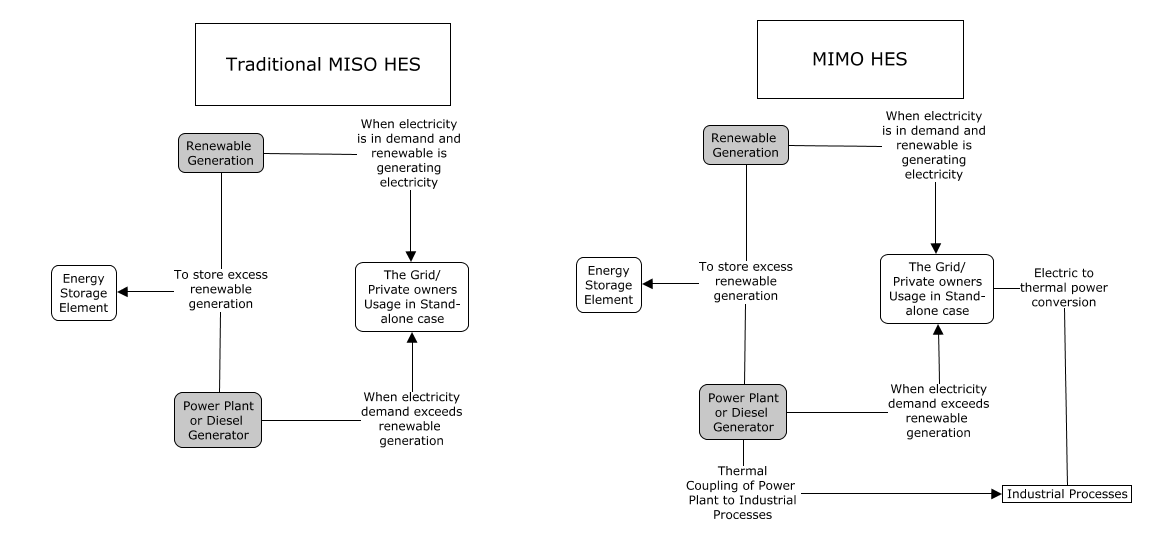
\includegraphics[width=\textwidth]{MISO_MIMO.png}
\caption{\small \sl This figure compares the MISO and MIMO configurations, demonstrating the differences between traditional hybrid energy systems that are focused on generating reliable electricity and non-traditional hybrid energy systems, which have the added objective of generating an additional product.  While many of the elements are the same, the MIMO system includes an Industrial Process  that is either thermally or electrically coupled.}
\end{figure*}

\section{Nuclear Renewable Hybrid Energy Systems}
Nuclear Renewable Hybrid Energy Systems (NRHES) are defined by Bragg-Sitton et al. (2014) as the

\begin{quotation}
"tighter coupling of nuclear and renewable energy sources in a manner that better optimizes energy use for the combined electricity, industrial manufacturing, and transportation sectors capable of apportioning thermal electrical energy to first meet the grid demand (with appropriate power conversion systems), then utilizing excess thermal and, in some cases, electrical energy to drive a process that results in an additional product \cite {Bragg-Sitton2014}".
\end{quotation}

The benefits to the participants of the NRHES that co-locate their facilities include minimizing system wide costs to the NRHES while increasing economic resilience by diversifying both the means of generating energy as well as the products produced. For example, if natural gas prices increase, the NRHES could rely less on the natural gas plant and put more focus on storage.  If short-term electricity prices are negative, the energy produced by the NRHES can be diverted to the industrial process.

The additional industrial products possible to couple in a NRHES include, but are not limited to: synthetic fuel, titanium, desalinated water, hydrogen, aluminum, and heat pumps \cite{Bienvenue2015}. The NPP diverts the energy it generates between the grid and the industrial process to maximize profit. The system can allocate energy based on the market value of each of the multiple outputs produced. In the case of a NPP coupled with a desalination plant, for example, if the price of electricity is low, more thermal and/or electric energy can be diverted to generate more clean water at a higher profit \cite {Chen2016}. The costs of running a dynamic system, such as the case with a NRHES, include additional wear and tear, decreased thermal efficiency  due to variability, and increased complexity of operations  \cite{Garcia2013}. The total net costs of the system, such as meeting regulatory expectations, have yet to be determined.

\section{Ongoing Modeling Research}
There have been no physical demonstrations to date of NRHES. Therefore, research has largely focused on computational modeling to determine the feasibility and optimization of coupling elements \cite{Rabiti2015, Boardman2013, Shropshire2012}. The literature review revealed that much of the work on NRHES is in the design and analysis stage \cite{Epiney2016, Boardman2013, Shropshire2012}. Research has focused on developing models that can dynamically simulate the contributions of variable energy sources, the constraints of fluctuating electricity demand, and thermal/electrical power demands for various industrial processes. The models focus on answering questions regarding minimizing the cost of electricity and ensuring profitability for each of the components comprising the NRHES. In order to move forward with development of any NRHES, such systems must demonstrate that they can be profitable and can reliably respond to fluctuating electricity production and demand \cite{Rabiti2015}.

An ongoing effort at \ac{inl}, \ac{anl}, and \ac{ornl} focuses on modeling a generic NRHES to optimize the size of the components as well as the overall functioning of the system. The generic nature of the plant means that regional variability in the renewable energy produced as well as the costs of the feedstocks for each of the systems is not taken into consideration. The generic model will test the economic viability of NRHES to determine if future development should be pursued. The industrial plant combines a nuclear power plant, a wind farm, a natural gas power plant, a battery, and a high temperature steam electrolysis hydrogen production facility. More component models will be developed in the future that can compare various industrial customers\cite{Harrison2016}. The chosen renewable source, a wind farm, models a highly stochastic system due to the unpredictable nature of wind generation \cite{Chen2016_wind}. The model optimizes the sizes of the nuclear power plant, the natural gas plant, and the battery. The model performs two optimizations, the first on the size of the components and the second optimizing the functioning of the system to minimize costs \cite{redfoot_rabiti_2018}. The objective is to choose the NRHES configuration that minimizes costs while meeting set emissions and grid reliability expectations.

\section{Computational Tools}
NRHES sit in an interesting location in computational modeling. There are many tools to model and optimize non-nuclear hybrid energy systems (HOMER, Hybrid2, SOLSIM, SOMES, ARES, RAPSIM, HOGA) \cite {Bernal-Agustin2009}. These programs calculate mass flow, electricity output, and the possible output of another product, such as hydrogen. Modelica and Excel, while neither specifically HES nor NRHES tools, have been used to model both nuclear and non-nuclear hybrid energy systems \cite{Shropshire2012, Chen2016, Binder2014, Garcia2015, Epiney2016}. HES tools have typically been developed for microgrid standalone systems. The main challenges to applying HES systems to a NRHES are the scale of the system being modeled and fluctuating grid demand.

\section{NRHES Models}
Selecting a tool to model a NRHES requires understanding what characteristics a model must possess in order to provide accurate information. For example, as discussed below, it is important for a NRHES model to incorporate the dynamic nature of the system in order to include losses from the fluctuations in the system. Rabiti et al. (2015) discusses the important elements of a NRHES computational model in detail, describing the basic requirements of the software as a

\begin{quotation}

"computational representation of the thermal, mechanical, chemical, and electrical processes in the systems as process units, reactors, manufacturing plants, and energy delivery (to the appropriate point of interface with the market transaction, such as an electricity bus, or a product depot or distribution terminal where a commodity price is established)"\cite{Rabiti2015}.
\end{quotation}

The model in development by the national laboratories combines \ac{raven} for the stochastic and statistical aspects of the system, such as generating synthetic wind data and optimizing the systems, with Modelica for modeling the various components in the NRHES.

\subsection{Modelica}
Modelica is a widely used open source language for modeling large and complex systems composed of smaller component models. It is particularly optimized for modeling dynamic systems. Modelica has powerful libraries, such as Thermopower, that include the thermohydraulic modeling tools required for modeling mass flows in energy systems \cite{Binder2014}. The language is well-maintained, giving it the added benefits of having up-to-date documentation and a community that can provide support. Typically Modelica is run on the Dymola developer environment, a private tool developed by the creator of Modelica, Dr. Hilding Elmquist. Another option for running the Modelica language is the open source OpenModelica environment.

A Modelica HES model developed in Binder et. al. (2014) includes a nuclear reactor, two steam cycles, a chemical plant, and an electrical component \cite{Binder2014}. The products of this Modelica NRHES model are synthetic fuel and electricity. The model includes the ramp up stage when the reactor initially starts or is increasing from a lower load. The steam generator connected to the NPP determines which of its turbines to use depending on electricity demand, the 60\% turbine, the 30\% turbine, or the 15\% turbine, which can be used in unison. A pressure relief valve releases excess energy unused by the turbines. The wind generation is modeled using the Western Wind dataset from the \ac{nrel} for an unspecified region in Idaho. Each component in the model was tested individually before being combined. Using the individual component models, verifications were made for the system as a whole. The startup transient state of the model took much greater computation time due to the complex interrelations of the components. Generally, running a model of a NRHES in Modelica requires a control algorithm, a differential equation that controls how the dynamic system allocates heat. The profitability control algorithm can be adjusted to incorporate varying parameters such as the price of electricity or the cost of natural gas. The study concluded that Modelica, due to its ability to evaluate control algorithms, is an effective tool for dynamically modeling a HES. As a tool that is optimized for large dynamic systems, Modelica has been used more than any other tool to model NRHESs at this point.

\paragraph{RAVEN}


The RAVEN tool was initially built for probabilistic risk assessment. RAVEN, as a probabilistic tool, can do parametric and stochastic analyses of systems\cite{RabitiRAVEN}. For NRHES, RAVEN is used to run different wind energy generation paths in order to generate a statistically fair representation of how renewables, in this case wind power, would likely function over any given week. RAVEN can be used to produce data representing the most generic seasonal wind generation over a week. A typical week can be extrapolated to represent a given season. The process can be repeated over the different seasons, which can be extrapolated to represent a year. Using synthetic generated data instead of historic data avoids the critique that the model only represents past behavior and is thus inapplicable to future trends \cite{redfoot_epiney_2016}. RAVEN can also be used to determine high-risk time series samples to ensure that high risk scenarios are accounted for in the study. RAVEN can also do probabilistic assessments such as loss of load probability and sensitivity to uncertainty analysis.

Any future modeling efforts for a NRHES would benefit from complimenting the ongoing modeling effort. Currently, all of the physics models for the NRHES are built in Modelica. To benefit from the work already done, any additional software would need to be able to easily communicate with the Modelica modeling language.  The model would benefit from a tool that would communicate with other chemical and utility standard physics modeling tools. Future work would benefit from coupling with other physics modeling tools, allowing groups to take advantage of the existing infrastructure while using their physics model of choice.

\subsection{Distinct Capabilities}
There are certain characteristics of a physical NRHES which a computational model would need to reasonably assess the system as a whole. Table I below demonstrates the functions which are most commonly incorporated in a model. The below discussion details the extensive work that has been done determining why a dynamic system is important to a NRHES.

In Garcia et. al. (2013) and Du et. al. (2014), a dynamic approach to modeling hybrid energy systems (HES) is applied in order to appropriately address the impacts of flexible operation of the system due to variable renewable generation \cite{Garcia2013, Du2014}. In Du et. al. (2014), two optimization problems are addressed: the first minimizes variability in the HES through optimizing components of the HES system, and the second imposes operating and capital costs on the design variables. Garcia et. al. (2013) has a two-part series. The first applies and analyzes performance of a dynamic approach to modeling some of the physical components of a traditional and an advanced MIMO HES. The second paper focuses on economic effects using a dynamic approach, as opposed to time series or statistical analysis. Overall, both parts of the series focus on how a dynamic approach better models the high level of variability of a HES for output generation and profitability maximization \cite{Garcia2013}. The costs of operating in a flexible manner, dynamically allocating resources between multiple coupled systems, are substantial enough to require a simulation that precisely models the variability of the system \cite{Garcia2013, Shropshire2011, Locatelli2015}. The dynamic modeling at this point focuses on the dynamic transfer of energy to different sources, and how this impacts the economics and grid reliability. The physical impacts of the grid system have not yet been included in the most developed NRHES simulation, the national laboratory model \cite{Harrison2016}.  The dynamic allocation of the heat and electricity depending on the renewable generation and the grid demand is an essential characteristic of a NRHES.  Including factors such as how quickly the NRHES will be able to switch between providing energy to the industrial facility and the grid will impact determining the economic and physical values of the model.

\section{Small Modular Reactors}
For completeness, the use of \ac{smrs} both as tools for load following and as sources of process heat must be addressed. SMRs are generally defined as nuclear reactors under 300 MWe. SMR designs, such as that in development by NuScale, combine multiple small reactor modules. Multiple SMRs in combination are a promising possibility for NRHES.  With multiple reactors, individual modules can be assigned to meet the industrial process energy demand, with others solely used for electricity generation. Furthermore, as electricity demand grows, additional modules can be added to the industrial park. Multiple SMRs have a clear means of load following, simply by shutting down those reactors whose energy output is not required due to seasonal shifts and other demand factors. The modularity of the SMRs allows greater flexibility in the design of the industrial park.  Locatelli (2015) discusses the technical and economic feasibility of load following using multiple SMRs, applying the excess energy toward generating algae-biofuel and desalinated water \cite{Locatelli2015}. He discusses the benefits as well as drawbacks of an NRHES that includes a thermal desalination process. A desalination plant has the benefits of switching between a latent and producing state and generating a product that is readily stored. The main drawback is poor water quality and output level when the desalination unit restarts. In general, SMRs have multiple means of adjusting their electricity output to the grid including coupling with an industrial process.

The NuScale reactor, with proposed construction starting in 2025 at INL, has motivated research into different methods of fluctuating the amount of electricity sent to the grid \cite{Ingersoll2014, Ingersoll2015, Ingersoll2016, Ingersoll2014_1}. The NuScale reactor design, as can be seen in the figure below, combines twelve small pressurized water reactors into one large pool of water.  Each of the reactors is rated at 50 MWe,generating a combined 600 MWe. The NuScale reactor has been evaluated to thermally couple with oil refining processes, multiple desalination techniques, as well as hydrogen production \cite{Ingersoll2014}. Besides from thermally coupling and rerouting the energy from electricity generation to process heat applications, the NuScale reactors have furthermore been evaluated for loosely coupling with the Horse Butte Wind Farm in nearby Idaho Falls \cite{Ingersoll2015}.  The NuScale plant has multiple approaches to meet the fluctuating electricity demanded by the grid, which NuScale designates as NuFollow \cite{Ingersoll2015}.  The NuScale plant can take down one or more of the low power reactors, changing the power output of one or more modules for shorter changes in the grid demand due to changes in wind output, and sending the heat generated by the reactor straight to the condenser bypassing the power generating turbine cycle.
\begin{figure*}[h!]
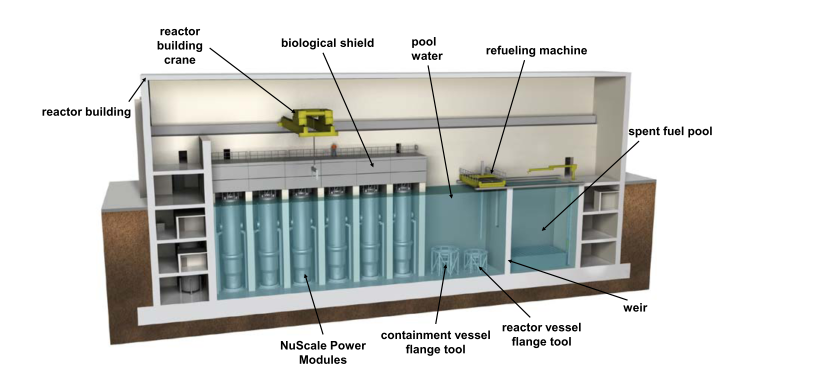
\includegraphics[width=\textwidth]{NuScale_cutaway.PNG}
\caption{\small \sl This figure displays the design of half of the NuScale module. Six of the reactor modules can be seen in the cooling pool along with the crane which inserts and removes the modules.}
\end{figure*}
\subsection{Other Research on NRHES Models}
Many more studies on HES and NRHES incorporate economic and technical modeling, but the essential characteristics of ability to model a dynamic and stochastic system have been covered. For completeness of the state of the art research on NRHES, some of the other relevant studies include:
\begin{itemize}
\item Shropshire et. al. (2012) does not focus on HES, but discusses how different models of flexible and small modular reactors could integrate into the European energy market with growing renewable generation, thus fulfilling the growing need for flexibility and load following in other electricity suppliers \cite{Shropshire2012}.
\item Shropshire et. al. (2011) develops target cost estimates for reactors given certain economic environments based on competing technology energy costs \cite{Shropshire2011}.
\item NEA-OECD (2011), Nuclear Energy Agency Organisation for Economic Co-operation and Development, presents an overview of the capability of implemented newer and older nuclear power plants to load follow \cite{Nuclear2011}.
\item Baker (2016) analyzes the \ac{lcoe} as the \ac{fom} and the role of battery storage to evaluate different NRHES scenarios \cite{Baker2016}
\item Kazimi et al. (2009) produces a preliminary dynamic analysis of two NRHES systems that have high levels of renewable energy generation and multiple outputs from the system. The study concludes that NRHES could lead to optimized energy use, reduced carbon, favorable economic performance, and flexible operation time \cite{Kazimi}.
\item Forsberg et. al. (2009) discusses using nuclear power to create more liquid transportation fuels from biomass and fossil fuel sources \cite{Forsberg2009}.
\item There have also been two regional modeling studies done on Texas and Arizona focused on including regional characteristics to determine the renewable used and the industrial process.
\end{itemize}
Table I displays the characteristics routinely described as necessary to model a NRHES along with their citations.

\begin{table}[h!]
\centering
\caption{References for Each NRHES Characteristic}
\begin{tabular}{ ||c | c|| }
 \hline
 NRHES Characteristic & Paper \\ [0.5ex]
 \hline \hline
 Dynamic & \cite{Garcia2013, Du2014, Kazimi, Garcia2016}\\
 \hline
 Sensitivity Analysis & \cite{Shropshire2011, Rehman2010, Adaramola2014, Chen2016}\\
 \hline
 Optimization of components & \cite{Chen2016,Ozcan2016, Forsberg2009,Garcia2015,Aumeier2011}\\
 \hline
 Stochastic Model of Renewables & \cite{Rabiti2015, Garcia2016,Locatelli2015}\\
 \hline
 Grid Demand model & \cite{Forsberg2013, Garcia2016,Garcia2013,Ruth2014,Chen2016}\\
 \hline
  Economic FOMs & \cite{Garcia2016,Chen2016,Rabiti2015,Epiney2016,Bragg-Sitton2014}\\
 \hline
\end{tabular}
\label{table:1}
\end{table}

The table displays the characteristics that arise as a pattern in many of the documents.  The six characteristics included in the table are those likely necessary for a NRHES model.  Each of the characteristics has been included in previous studies, and thus has some already proposed approaches.  The characteristics can be studied in greater detail in order to determine if they satisfactorily model the system.


\chapter{Applying Risk Assessment Techniques to NRHES}
\label{Risk}
Identifying likely failures is an important aspect of safe and secure operation of any large infrastructure. For a NRHES, a large piece of infrastructure that has as of yet to be built, a design that addresses likely failures ensures long term safe, reliable, and profitable operation. This chapter will evaluate the economic, grid reliability, and physical risks of failures in the coupling of a nuclear power plant to an industrial process which functions in a dynamic fashion. Three preliminary hazard analyses will initially be applied to the safety, ability to fluctuate, and profitability of the system in order to do a cursory qualitative model of what concerns need to be taken into consideration. A fuzzy Analytic Hierarchy Process (f-AHP) will then be applied to various industrial process options to couple with an NRHES. The focus of this section is to develop a means of comparing various NRHES industrial processes to determine which industrial process will be used in the exergy analysis.
\section{Risk Assessment Background}
Risk assessment is a means of analyzing complex systems for hazards. Often the risk assessment tools; such as probabilistic risk assessment, fault tree analysis, and failure mode and effects analysis; model many variables in large systems and attempt to contain them into an easy to understand table or number for comparison. Since there has yet to be a physical model of a NRHES built, now is the appropriate time to assess risks in order to incorporate mitigating measures in the design basis. Incorporating risk management in the design of a facility minimizes the costs and dangers associated with the system in the long run.
%When determining an appropriate electricity generation source for a given region it is important to incorporate variables such as economic viability, emissions, flexibility, and reliability. A NRHES is even more difficult to quantify as it supplies both electricity to the grid as well as a secondary product. The goal is to have a more economically robust system that emits less and is both more reliable and more flexible than any electricity generation source currently available.

\section{Preliminary Hazards Analysis}
As was done in Falcone et. al. in establishing a new approach to risk assessment of cogeneration systems, this risk assessment will begin with a \ac{pha} \cite{Falcone}. The main purpose for a PHA is, as the name suggests, identify hazards and possible implications of the design of a particular system or product.  A PHA is appropriate for the current state of development for a NRHES due to it still being in the design stage. The goal of this PHA will be to highlight potential economic, reliability, and physical safety hazards. Performing a PHA at this early point in the life cycle of a NRHES will hopefully reduce the resources spent on engineering design and potential construction errors. This analysis is not exhaustive but will address some of the more obvious concerns. The PHA will need to be added upon as research continues and hazards are determined.
	In order to perform a PHA requires classifying the hazard level and frequency associated with each event. The hazard classes for this PHA range from Negligible to Catastrophic. A Class I hazard has negligible negative outcomes, a Class II hazard has marginal effects, a Class III hazard has critical impacts, and a Class IV hazard has catastrophic impacts\cite{ostrom2012risk}.  The frequency of occurrence, since this system has yet to have a physical demonstration, will be qualitative as the values cannot be verified at this point. A discussion of the tables follows after tables \ref{econ}, \ref{fluc}, and \ref{safety} below.

\begin{landscape}
%\subsubsection{Economic PHA}
\begin{table}[h!]
\centering
\caption{Economic Preliminary Hazard Analysis}
\label{econ}
\begin{tabular}{|l|l|l|l|l|l|}
\hline
\textbf{\begin{tabular}[c]{@{}l@{}}Potential \\ Failure\end{tabular}} & \textbf{\begin{tabular}[c]{@{}l@{}}Event Causing\\ Hazardous\\ Condition\end{tabular}} & \textbf{\begin{tabular}[c]{@{}l@{}}Hazardous\\ Condition\end{tabular}}  & \textbf{Hazard Class} & \textbf{\begin{tabular}[c]{@{}l@{}}Preventative \\ Measure\end{tabular}} & \textbf{\begin{tabular}[c]{@{}l@{}}Qualitative\\ Likelihood\end{tabular}} \\
\hline
\begin{tabular}[c]{@{}l@{}}Industrial process\\ is not profitable \end{tabular}      & \begin{tabular}[c]{@{}l@{}}If the industrial\\ process has to be\\ ready to take load\\ from the grid, it \\ will likely be running\\ below capacity and \\ may not be profitable\end{tabular}      & \begin{tabular}[c]{@{}l@{}}Industrial \\ process loosing\\ money\end{tabular} & \begin{tabular}[c]{@{}l@{}}Class III,\\ the benefit of\\ the NRHES \\ would be lost\\ without a means\\ of having the \\ industrial process\\ prepared to take \\ heat. \end{tabular}    & \begin{tabular}[c]{@{}l@{}}Contracts \\ ensuring\\ a certain profit\\ for the industrial\\ process to be \\ prepared to \\ take heat from\\ the Nuclear\\ Power Plant\end{tabular} & Likely \\
\hline
\begin{tabular}[c]{@{}l@{}}Nuclear regulations \\ could apply to the\\ whole system, \\ increasing the costs\\ of the system\end{tabular} & \begin{tabular}[c]{@{}l@{}}Since the \\ components will \\ be co-located \& \\ coupled, the NRC \\ may have\\ jurisdiction \\ over the whole system\end{tabular}  & \begin{tabular}[c]{@{}l@{}}Additional \\ regulations \\ on the industrial \\ process could \\ result in greater\\ costs\end{tabular} & \begin{tabular}[c]{@{}l@{}}Class III: without an \\ industrial process\\ the whole NRHES \\ would be undermined.\end{tabular} & \begin{tabular}[c]{@{}l@{}}Determine regulatory \\ oversight before \\ beginning \\ construction\end{tabular} & \begin{tabular}[c]{@{}l@{}}Fairly Likely\\ as the other\\ components\\ would be\\ within the\\ required \\ boundary \\ around the NPP\end{tabular} \\
\hline
\begin{tabular}[c]{@{}l@{}}Feedstock\\ Costs Rising \end{tabular} & \begin{tabular}[c]{@{}l@{}}Any of the feedstocks\\  could rise in price for \\ any number of reasons. \\ Rise in price during \\ the operation of the \\ system could result in \\ the product prices no \\ longer being\\ competitive\end{tabular} & \begin{tabular}[c]{@{}l@{}}Feedstocks rising in \\ price during the \\ operation of the system \\ could\\ result in the \\ product prices no \\ longer being \\ competitive\end{tabular} & \begin{tabular}[c]{@{}l@{}}Class I: shifts \\ already occur in\\ feed stock prices and\\ are systems adjust.\end{tabular}  & \begin{tabular}[c]{@{}l@{}}Include long term \\ projections for the \\ feedstock costs of \\ the various \\ components in the \\ design phase of the \\ NRHES\end{tabular}                      & \begin{tabular}[c]{@{}l@{}}Likely there \\ will be \\ fluctuations.\\ Depends on the \\ feedstock\end{tabular}\\
\hline
\begin{tabular}[c]{@{}l@{}}Product Value\\Decreasing\end{tabular} & \begin{tabular}[c]{@{}l@{}}There could be a \\ change in \\ conditions or a \\ new technology \\ that makes the \\ industrial process \\ product value \\ decrease\end{tabular} & \begin{tabular}[c]{@{}l@{}}For each of the products,\\ the reason would be \\ different. Desal: a \\ drought could end\\ Syn fuel: oil prices \\ could decrease\\ Hydrogen: Less \\ energy\\ intensive \\ process could be \\ invented\end{tabular} & \begin{tabular}[c]{@{}l@{}}Class II: the industrial \\ process would need\\ to be further subsidized\\ by other components \\ to continue to run\end{tabular}& \begin{tabular}[c]{@{}l@{}}Do long term \\ economic \\ analysis of the \\ industrial \\ process. Pick \\ a product \\ or location where\\ the product will \\ clearly be in demand\end{tabular} & \begin{tabular}[c]{@{}l@{}}Possible: The \\ product value \\ will likely \\ fluctuate over \\ the length of \\ the\\ project\end{tabular}          \\ \hline
\end{tabular}
\end{table}                                           \end{landscape}



\begin{landscape}
%\subsection{Grid Reliability PHA}
\begin{table}[h!]
\centering
\caption{Grid Reliability Preliminary Hazard Analysis}
\label{fluc}
\begin{tabular}{|l|l|l|l|l|l|}
\hline
\textbf{\begin{tabular}[c]{@{}l@{}}Potential \\ Failure\end{tabular}} & \textbf{\begin{tabular}[c]{@{}l@{}}Event Causing\\ Hazardous\\ Condition\end{tabular}} & \textbf{\begin{tabular}[c]{@{}l@{}}Hazardous\\ Condition\end{tabular}} & \textbf{Hazard Class} & \textbf{\begin{tabular}[c]{@{}l@{}}Preventative \\ Measure\end{tabular}}  & \textbf{\begin{tabular}[c]{@{}l@{}}Qualitative\\ Likelihood\end{tabular}} \\
\hline
\begin{tabular}[c]{@{}l@{}}Nuclear Power \\ Plant Outage\end{tabular}  & \begin{tabular}[c]{@{}l@{}}The NPP needs \\ to be refueled\end{tabular} & \begin{tabular}[c]{@{}l@{}}NPP down for \\ refueling\end{tabular} & \begin{tabular}[c]{@{}l@{}}Class I: This will \\ be a routine issue. \\ The industrial \\ process will need \\ to stop during the \\ outage and the \\ grid will need to \\ get electricity \\ from peaker\\ plants\end{tabular} & \begin{tabular}[c]{@{}l@{}}Plan ahead with the \\ industrial process \\ so that it can either \\ get\\ electricity from\\ the grid or be \\ paid to close for \\ the outage.\end{tabular}                                     & \begin{tabular}[c]{@{}l@{}}Certain: an \\ NPP needs to \\ be refueled\end{tabular} \\
\hline
\begin{tabular}[c]{@{}l@{}}System not able \\ to quickly shift\\  heat from \\ industrial process \\ to\\ electricity \\ generation\end{tabular} & \begin{tabular}[c]{@{}l@{}}The NPP heat \\ transport system \\ taking a while to \\ shift.\end{tabular} & \begin{tabular}[c]{@{}l@{}}The NRHES is \\ briefly unable \\ to meet \\ the grid demand\end{tabular} & \begin{tabular}[c]{@{}l@{}}Class II: There \\ would be some \\ money loss as \\ some other \\ electricity \\ generation system \\ would supply the \\ demanded energy \\ during the transition \\ period\end{tabular}            & \begin{tabular}[c]{@{}l@{}}Include the time it \\ takes to allocate \\ heat in models of \\ the NRHES to \\ determine how \\ much of a limiting \\ factor it is likely to be.\\ Include a battery in\\ the NRHES\end{tabular} & Likely \\                       \hline
\end{tabular}
\end{table}
\end{landscape}



\begin{landscape}
%\subsection{Physical PHA}
\begin{table}[h!]
\centering
\caption{Physical Preliminary Hazards Analysis}
\label{safety}
\begin{tabular}{|l|l|l|l|l|l|}
\hline
\textbf{\begin{tabular}[c]{@{}l@{}}Potential \\ Failure\end{tabular}}                        & \textbf{\begin{tabular}[c]{@{}l@{}}Event Causing\\ Hazardous\\ Condition\end{tabular}} & \textbf{\begin{tabular}[c]{@{}l@{}}Hazardous\\ Condition\end{tabular}} & \textbf{Hazard Class} & \textbf{\begin{tabular}[c]{@{}l@{}}Preventative \\ Measure\end{tabular}} & \textbf{\begin{tabular}[c]{@{}l@{}}Qualitative\\ Likelihood\end{tabular}}                 \\
\hline
\begin{tabular}[c]{@{}l@{}}Materials failure \\ in the heat \\ transport system\end{tabular} & \begin{tabular}[c]{@{}l@{}}NRHES are very \\ dynamic systems. \\ There will likely \\ be greater materials \\ wear due to the \\ dynamisticity of \\ the system\end{tabular} & \begin{tabular}[c]{@{}l@{}}Heat transport \\ pipe forms a leak\end{tabular}            & \begin{tabular}[c]{@{}l@{}}Class III:There \\ would be a loss \\ of\\ money due \\ to the shutdown \\ of the system\end{tabular}                                                                                                          & \begin{tabular}[c]{@{}l@{}}Reliable maintenance \\ \& appropriate choice \\ of heat transport \\ system\\ materials\end{tabular} & Possible                                                                                  \\
\hline
Release of Radionuclides                                                                     & \begin{tabular}[c]{@{}l@{}}Radionuclides \\ would need to \\ escape first into \\ the heat transport \\ system and then from \\ the heat transport system \\to the environment\end{tabular}                                                                                          & \begin{tabular}[c]{@{}l@{}}A large release \\ of airborne\\ radionuclides\end{tabular} & \begin{tabular}[c]{@{}l@{}}Class IV: A \\ radiation release \\ that could \\ potentially impact \\ human health \\ would have\\ massive negative \\ impacts for the \\ nuclear industry \& \\ would shut down \\ the\\ NRHES\end{tabular} & \begin{tabular}[c]{@{}l@{}}Passive safety \\ systems, excellent \\ safety culture, \\ good reactor design\end{tabular}           & \begin{tabular}[c]{@{}l@{}}Unlikely: Based \\ on history of \\ NPP operation\end{tabular} \\
\hline
\end{tabular}
\end{table}
\end{landscape}

The initial economic PHA, table \ref{econ}, demonstrates the importance of having detailed agreements between the various members of a NRHES industrial park before construction begins.  Likely, the whole system would function better under a single owner.  A single owner could allow an aspect of the NRHES, such as the industrial process, to loose money and still be economic overall. Further avenues which need to be investigated before the construction of an industrial park include understanding the regulatory impacts and the long term projected worth of the products generated.

The initial grid reliability PHA, table \ref{fluc}, demonstrates the importance of understanding how coupling an NPP to an industrial process will require a change of the scheduling approach to a nuclear power plant. Nuclear power plants require immense amounts of planning and scheduling in order to ensure safe operation of the plant.  Increasing the complexity through coupling the nuclear power plant to other systems will increase the complexity of scheduling activities such as outages as well as optimizing the heat and electricity output of the system to match the grid demand.

The initial physical PHA, table \ref{safety},  demonstrates how, if done correctly, a thermally coupled industrial process to a nuclear power plant does not have to increase the danger of the system.  Since nuclear power plants already have a lot of techniques in place to ensure a safe system that will not harm the public or the environment, those same approaches should be applied to the thermally coupled system. The existing infrastructure, including the safety culture, could be extended to the thermal coupling. Thermal coupling is used throughout this thesis as the use of heat from the \ac{npp} used directly for an industrial process.  Electrical coupling, for comparison, takes the electricity generated by the \ac{npp} which is then used to do electrical work or converted into heat or mechanical work to produce the desired product in the industrial process.


\section{Analytic Hierarchy Process}
The fuzzy AHP done in this research compares NRHESs that include thermal coupling to three types of industrial processes: desalination, synthetic fuel production, and hydrogen production.  The AHP evaluates the profitability, flexibility, and safety characteristics in the coupling of a nuclear power plant to each of the given industrial processes. While AHP has been applied to energy systems in the literature, the application to NRHES is novel. An AHP approach provides important information into design considerations and quantitatively approaches, through expert opinion, which alternative is likely to be strongest given the criteria chosen. As NRHESs are currently in the research and development stage, AHP is a beneficial tool to develop for future decision making for NRHES.

An AHP uses pairwise comparisons of various potential options depending on a set of predetermined characteristics. Originally developed in the 1970s by Thomas L. Saaty, AHP has been applied to everything from determining appropriate bridge construction \cite{Pan2008}, to the appropriate energy make-up of Turkey\cite{Kahraman2010} \cite{Saaty1987}. AHP is a multicriteria decision-making tool. There is a wealth of research applying multicriteria decision-making tools to energy planning. Pohekar et al. reviewed more than 90 published papers on multi-criteria decision making and energy planning \cite{Pohekar2004}. Pohekar et al. found AHP to be the most popular multicriteria decision-making technique used in energy planning. The reasons for the prevalence of AHP in energy planning, Pohekar et al. suggests, is due to its ability to:
\begin{quote}
	"convert a complex problem into a simple hierarchy, flexibility, intuitive appeal, its ability to mix qualitative as well as quantitative criteria in the same decision framework and use of computational aids leading to successful decisions in many domains.\cite{Pohekar2004}"
 \end{quote}
Some of the previous applications of AHP to energy systems noted in Pohekar et al. include Akash et al.  1999; and Ramanathan et al. 1995. Akash et al. uses AHP to analyze the selection of power plants in Jordan \cite{Akash1999}.  Ramanathan et al. applies AHP at a household level in India to determine which energy resources work best for various tasks in the home such as heating, water pumping, lighting, and household appliances \cite{Ramanathan1995}.

The general process for applying AHP involves initially determining a set of alternatives and a set of criteria on which to compare the alternatives. The hierarchy comes from the objective being structured above the criteria, which is then structured above the alternatives, as can be seen in figure 3.1 below. To find the relative value of one of the alternatives over the other, the AHP approach develops a series of pairwise comparisons creating a ratio scale.  Generally AHP is done on a scale of one to nine. After creating the ratio scale, the AHP approach applies an eigenvalue method to include the relative weights of each of the criteria to each of  the elements. Finally, the relative weights are combined with the ratios forming one measurement to compare the various elements.

\begin{figure}[h!]
  \centering
  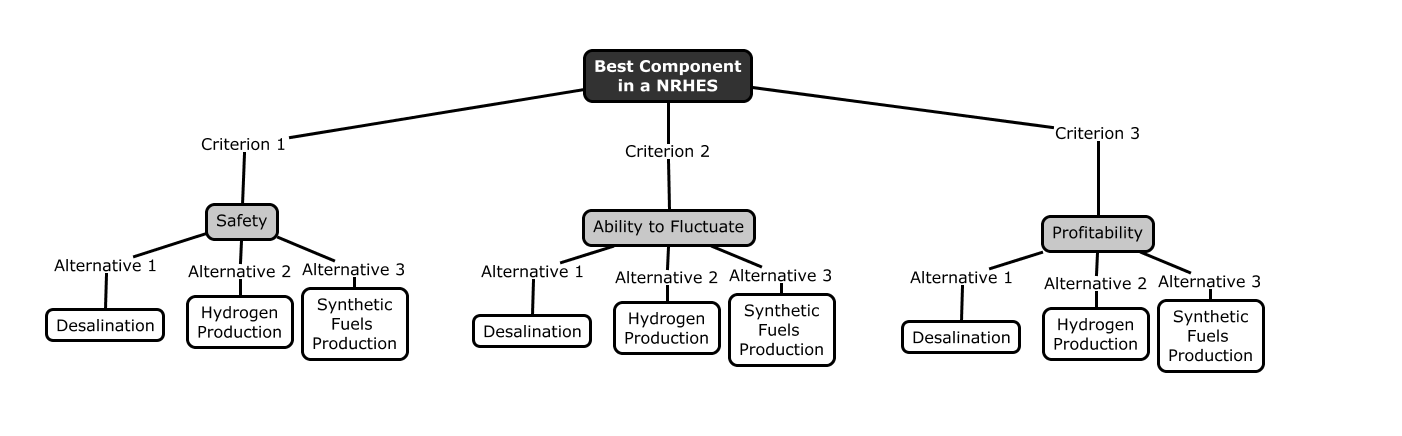
\includegraphics[width=0.9\textwidth]{AHP_hierarchy.PNG}
  \caption{A figure displaying the overall hierarchy of the industrial processes under evaluation for inclusion in the NRHES}
\end{figure}

The AHP provides not only insight into which is the best overall choice given the inputs and weights, but also which is the strongest candidate for each of the criterion. During the AHP process, before aggregating the values into one measurement, there are clear measurements of each of the alternatives in each of the criterion. The subjective nature of expert judgment as data requires a means of evaluation. As a check on the validity of the data,a traditional AHP measures the consistency of the values given by the experts using a Consistency Ratio, which needs to be less than .1, or 10\%, in order to be considered consistent. The Consistency Ratio compares the randomness of the expert judgments to a Random Consistency Index \cite{Saaty1987}.  If the consistency ratio is greater than .1, the data is judged to be too close to random.


\section{Fuzzy AHP}
Fuzzy logic applied to AHP takes into consideration the uncertainty inherent in a small number of expert opinions. Fuzzy AHP is an extension of the original AHP developed by Saaty in the 1970s \cite{Saaty1987}. Since Saaty's original development of AHP, multiple means of fuzzy AHP have emerged. Some notable fuzzy AHP approaches, as noted in \cite{Kahraman2010} include:
\begin{itemize}
\item Van Laarhoven and Pedrycz's approach from 1983 using triangular membership functions
\item Buckley's 1985 use of trapezoidal membership functions to determine fuzzy priorities
\item Cheng's 1997 approach focused on the grade value of the membership function.
\item Kahraman et al. generated a fuzzy weighted evaluation \cite{Kahraman2010}
\item Chang presented a new approach first determining triangular fuzzy numbers, then applying extent analysis method \cite{Chang1996}
\end{itemize}

 In the Buckley approach to fuzzy AHP, which is applied in this paper, $\alpha$ represents a value between zero and one reflecting the uncertainty.  Uncertainty is greatest when $\alpha$ is close to zero and least when close to one. As can be seen in the figure below, in a trapezoidal membership approach, the lower left point of the triangle, where $\alpha$ equals zero, is the minimum fuzzy number, the points making up the middle represent the most likely fuzzy number, and the point at a y value of zero on the right represents the maximum fuzzy number \cite{Pan2008}. The higher the fuzzy number on the x axis, the more important that criteria is, or the stronger the alternative.
\begin{figure}[h!]
  \centering
  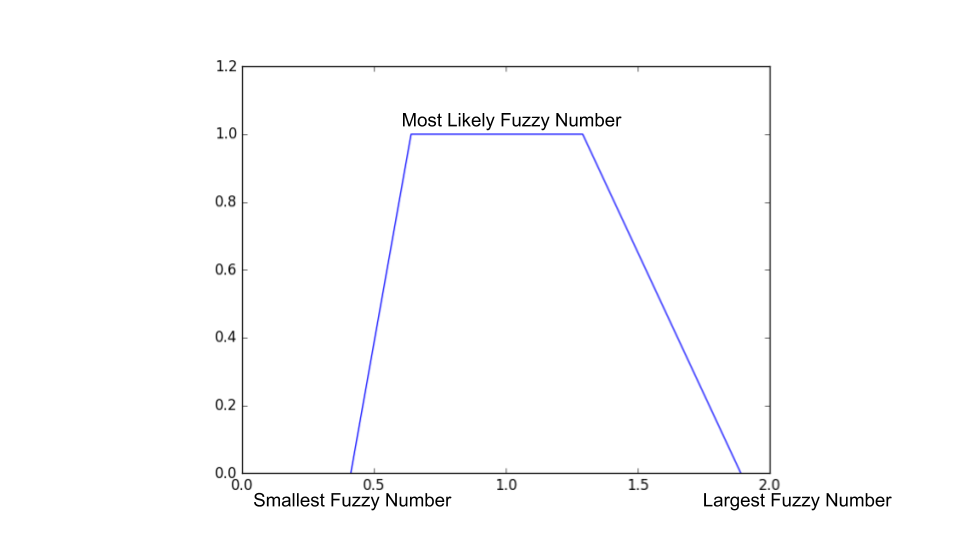
\includegraphics[width=0.9\textwidth]{Fuzzy_explaination.png}
   \caption{A figure displaying the meaning behind the membership function graph for the fuzzy numbers}
\end{figure}

 As described in \cite{Kahraman2010}, after receiving the numbers from the decision makers, the fuzzy weight can be found by determining the geometric mean for each row in each of the AHP matrices:

 \begin{equation}
 z_i=[\prod_{j=1}^n t_{ij}]^{\frac{1}{n}}
 \end{equation}

 Where $t_{ij}=(a_{ij},b_{ij}, c_{ij}, d_{ij})$ correspond to the fuzzy values in Table 1 below. $n$ is the number of values in each row.  For example, if three experts were taking a survey with three pairwise comparisons, there would be nine total answers in each row. To find the performance scores ($r$), first sum each of the geometric means in each row, then weight each of the values accordingly:

\begin{equation}
r_{ij}=(\frac{a_i}{d},\frac{b_i}{c},\frac{c_i}{b},\frac{d_i}{a})
\end{equation}

To find the fuzzy utility:

\begin{equation}
U_i=\sum_{j=1}^n w_j*r_{ij}
\end{equation}

where w is the weight found by the comparison of the importance of the various criteria to one another. To find the membership function $M(x)$, take the lowest value of the utility set and set the membership function to zero.  For the middle values of the utility set, the membership function is one. For all values greater than the greatest member of the utility set, the membership function is zero. For a utility set $(x_1,x_2,x_3,x_4)$

\begin{center}
\begin{tabular}{ |c|c| }
 \hline
 x & M(x)\\
 \hline
 $\leq x_1$  & 0 \\
 $\geq x_4$ & 0  \\
 $x_2 \leq x \leq x_3$ & 1  \\
 $x_1 \leq x \leq x_2$ & $\alpha \in [0,1]$\\
 $x_3 \leq x \leq x_4$ & $\alpha \in [0,1]$\\
 \hline
\end{tabular}
\end{center}

\begin{table}[h!]
\centering
\caption{Fuzzy Logic Value Mapping}
\label{Fuzzy values}
\begin{tabular}{|l|l|l|}
\hline
\textbf{Description }                                                           & \textbf{Values }       & \textbf{Inverse}           \\
\hline
Equal                                                                  & (1, 1, 1, 1)     & (1, 1, 1, 1)         \\
\hline
Equal Importance                                                       & (1/2, 3/4, 5/4, 3/2) & (2/3, 4/5, 4/3, 2)      \\
\hline
Weak Importance                                                        & (1, 3/2, 5/2, 3)   & (1/3, 2/5, 2/3, 1)   \\
\hline
Strong Importance                                                      & (2, 5/2, 7/2, 4)     & (1/4, 2/7, 2/5, 1/2) \\
\hline
\begin{tabular}[c]{@{}l@{}}Very Strong\\ Importance\end{tabular}       & (5, 11/2, 13/2, 7)     & (1/7, 2/11, 2/13, 1/5) \\\hline
\begin{tabular}[c]{@{}l@{}}Absolutely Strong\\ Importance\end{tabular} & (7, 15/2, 17/2, 9)     & (1/9, 2/17, 2/15, 1/7)\\
\hline
\end{tabular}
\end{table}

\section{Expert AHP Survey}
The objective for the expert AHP survey is to determine the optimal industrial process to include in a generic NRHES industrial park based on three criteria. The industrial process options are desalination, high temperature steam electrolysis, and synthetic fuel production. The criteria the options are judged on are ability to fluctuate, safety, and profitability. The optimal way to perform an Analytic Hierarchy Process (AHP) is to gather a group of experts with complementary specializations in a general field to discuss the relative values of various options under determined criteria. For example, performing an AHP to determine the optimal industrial process in a NRHES would best be done by gathering a group of experts in NRHESs with specialties in understanding each of the specific industrial processes. The group could discuss the relative values to give to each of the alternatives for a given criterion. Due to the struggles of getting a group of NRHES experts together in the same place, the values found for this research came from sending a survey to experts.  Other AHP evaluations employ similar methods\cite{Pan2008}. For this research, an expert is defined as someone who has published research or reports on NRHES.

	I chose the alternatives of desalination, hydrogen production, and synthetic fuels production due to their prominent role in research surrounding NRHES \cite{Bragg-Sitton2014,Locatelli2015,Kim2016,Bragg-Sitton2016,Garcia2016,Shropshire2011, Ruth2014,Bienvenu2015}.  I chose the criterion of ability to fluctuate as the industrial process in a NRHES will need to be able to fluctuate to adjust to change demand as well as the dynamic generation from the industrial process.  I chose the criterion of safety due to the inherent need for safety, especially within the context of the nuclear safety culture.  Safety underlies both the characteristic of ability to fluctuate and profitability. If the industrial process is not safe, it will not run, and therefore the other two characteristics are negligible. I chose profitability as clearly the whole NRHES will need to be profitable in order to continue to run.  The industrial process provides a secondary source of income  increasing the overall profitability of the system as a whole.

There were five experts who completed the Analytic Hierarchy Process for a Nuclear Renewable Hybrid Energy System survey. Due to the small number of experts included in the survey, a fuzzy systems approach has been applied to the AHP. Tsyganok et al. determined that the expert competence should always be taken into consideration, especially when there are less than 50 experts included in the evaluation \cite{Tsyganok2012}. Thus in this case a fuzzy approach is clearly applicable due to the low number of responses.

 For this research, the same NRHES with only the industrial process switched out will be compared. The assumptions for this research include:
\begin{itemize}
\item The process used for hydrogen production is high temperature steam electrolysis with thermal as well as electrical coupling to the nuclear power plant
\item  The process for desalination is thermal desalination through distillation directly using heat from the nuclear power plant
\item The synthetic fuel process is a Fischer-Tropsch method using coal as the hydrocarbon source
\item Each of the processes consumes the same amount of heat from the nuclear power plant
\item All of the industrial processes are thermally coupled
\item Regional accessibility of feedstocks for each of the industrial processes are the same
\item Regional transportation costs are the same
\item Regulatory and taxation costs are the same
\end{itemize}

As can be seen in Table 2 below, the scale for the answers for the second part of the question ranged from two to  nine.  In the initial question the expert determines which of the alternatives better fits the criteria.  If the two alternatives were judged to equally answer the question, then a value of 1 was assigned to the relative importance of both. Table 3.5 displays the relative values for each of the characteristics considered in the AHP. The values are chosen on a scale of one to nine, with the industrial process strongly reflecting that characteristic receiving a nine and the characteristic relatively less reflecting those characteristics receiving appropriate smaller numbers. While the safety of the system is in reality the most important characteristic, as it is the foundation which the economic and grid reliability characteristics rely on, the safety issues are the most easy to mitigate and the most well known.

\begin{table}[h!]
\centering
\caption{Example of questions given in the Expert AHP survey}
\label{AHPQuestions}
\begin{tabular}{l}
Questions included in the expert AHP survey:                                                                                   \\ \hline
\multicolumn{1}{|l|}{\begin{tabular}[c]{@{}l@{}}Q1a: Do you think that the ability to fluctuate,is more important\\ than profitability of an industrial process?\\ Q1b: From 2 to 9, how would you compare the importance of \\ safety of an industrial process to the ability of the industrial process to fluctuate?\\ Q2a: Do you think that the ability to fluctuate,is more important than \\ profitability of an industrial process?\\ Q2b: From 2 to 9, how would would you compare the importance \\ of safety of an industrial process to the ability of the industrial process to fluctuate?\end{tabular}} \\ \hline
\end{tabular}
\end{table}

\begin{table}[h!]
\centering
\caption{AHP Scale Description}
\label{AHPScale}
\begin{tabular}{|l|l|l|}
\hline
Quantitative Value & Explanation                                                                                                                              & Verbal Judgement                                                        \\ \hline
1                  & \begin{tabular}[c]{@{}l@{}}They are equally important \\ or equally meet the criterion\end{tabular}                                      & Equally more important                                                  \\ \hline
2                  & \begin{tabular}[c]{@{}l@{}}Experience and judgement \\ favor one alternative over \\ the other by a small margin\end{tabular}            & Weakly more important                                                   \\ \hline
3                  & \begin{tabular}[c]{@{}l@{}}Experience and judgement \\ moderately favor one \\ alternative over the other\end{tabular}                   & Weakly more important                                                   \\ \hline
4                  & \begin{tabular}[c]{@{}l@{}}Experience and judgement \\ clearly favor one \\ alternative over the other\end{tabular}                      & Strongly more important                                                 \\ \hline
5                  & \begin{tabular}[c]{@{}l@{}}Experience and judgement \\ strongly favor one \\ alternative over the other\end{tabular}                     & Strongly more important                                                 \\ \hline
6                  & \begin{tabular}[c]{@{}l@{}}Practice suggests moderate\\ preference for one alternative \\ over the other\end{tabular}                    & \begin{tabular}[c]{@{}l@{}}Very strongly more\\ important\end{tabular}  \\ \hline
7                  & \begin{tabular}[c]{@{}l@{}}One alternative is favored \\ very strongly over the other \\ and has been shown in practice\end{tabular}     & \begin{tabular}[c]{@{}l@{}}Very strongly more \\ important\end{tabular} \\ \hline
8                  & \begin{tabular}[c]{@{}l@{}}It is fairly clear that, in practice\\ one alternative is better than the \\ other\end{tabular}               & \begin{tabular}[c]{@{}l@{}}Absolutely more \\ important\end{tabular}    \\ \hline
9                  & \begin{tabular}[c]{@{}l@{}}The evidence favoring one \\ alternative over the other is of\\ the highest possible affirmation\end{tabular} & \begin{tabular}[c]{@{}l@{}}Absolutely more \\ important\end{tabular}    \\ \hline
\end{tabular}
\end{table}

\section{AHP Results and Discussion}
As can be seen in table 4, the utility set values which comprise the membership function are highest for desalination. The utility set generates the weighted value for each of the alternatives using the geometric mean method discussed above. As the higher the utility the greater the value, desalination ranks highest of the options for an industrial process given the criteria. As can be seen in Table 5, safety clearly was prioritized.  Due to the high value placed on safety, and the sense that desalination is safer than the alternatives, it follows that it has a greater fuzzy number. Clearly, the heavy weight placed on safety played a major role in determining the outcome.

While AHP provides a means to compare various options and criteria, it is limited by not including vital information surrounding when a certain standard has been met. In the case of this research, safety and flexibility standards could have been fully met by all of the industrial processes. Safety, instead of being a relative point of comparison, may be better treated as a set of standards to be achieved, such as those presented in the International Organization for Standardization standards for cogeneration \cite{ISO2017}. While desalination is perceived to be a safer industrial process, that does not mean that a synthetic fuel upgrading system or a high temperature steam electrolysis plant is unsafe to couple to a nuclear power plant. The fact that desalination is perceived as safer and more able to fluctuate becomes negligible at that point. AHP is a beneficial tool when determining the relative value between alternatives.  For example, profitability is a valuable characteristic to compare on relative terms.

NRHESs are difficult systems to have a fully developed sense of expertise surrounding. Due to the industrial parks including different components as well as the importance of including technical, economic, and political variables in the decision making. While an AHP is a valuable tool because it is able to include a variety of characteristics from different disciplines, there need to be experts representing each of the disciplines. Furthermore, the more experts included in the survey, the stronger the data and the more likely a valid conclusion can be drawn from the data.
\begin{table}[h!]
\centering
\caption{Utility Set values for each of the industrial processes}
\label{utility}
\begin{tabular}{|l|l|}
\hline
\begin{tabular}[c]{@{}l@{}}Industrial \\ Process\end{tabular} & Utility Set               \\ \hline
Desalination                                                  & (0.412, 0.641, 1.291, 1.891) \\ \hline
\begin{tabular}[c]{@{}l@{}}Hydrogen\\ Production\end{tabular} & (0.029, 0.047, 0.084, 0.136) \\ \hline
\begin{tabular}[c]{@{}l@{}}Synthetic \\ Fuels\end{tabular}    & (0.086, 0.128, 0.265, 0.437) \\ \hline
\end{tabular}
\end{table}




\begin{table}[h!]
\centering
\caption{Performance Scores of Safety for the various industrial processes included}
\label{my-label}
\begin{tabular}{|l|l|}
\hline
Industrial Process                                                    & Safety Performance Score     \\ \hline
Desalination                                                           & (0.309,0.424, 0.708, 0.917)  \\ \hline
\begin{tabular}[c]{@{}l@{}}Hydrogen \\ Production\end{tabular}        & (0.118, 0.162 ,0.277 ,0.390) \\ \hline
\begin{tabular}[c]{@{}l@{}}Synthetic Fuels \\ Production\end{tabular} & (0.139, 0.181, 0.317, 0.459) \\ \hline
\end{tabular}
\end{table}

\begin{table}[h!]
\centering
\caption{Ability to Fluctuate Performance Scores for the various industrial processes included}
\label{P-ScoreFlux}
\begin{tabular}{|l|l|}
\hline
\begin{tabular}[c]{@{}l@{}}Industrial \\ Process\end{tabular} & \begin{tabular}[c]{@{}l@{}}Ability to Fluctuate \\ Performance Scores\end{tabular} \\ \hline
Desalination                                                  & (0.328, 0.436, 0.687, 0.868)                                                       \\ \hline
\begin{tabular}[c]{@{}l@{}}Hydrogen\\ Production\end{tabular} & (0.183, 0.234, 0.365, 0.496)                                                       \\ \hline
\begin{tabular}[c]{@{}l@{}}Synthetic \\ Fuels\end{tabular}    & (0.104, 0.129, 0.199, 0.262)                                                       \\ \hline
\end{tabular}
\end{table}

\begin{table}[h!]
\centering
\caption{Profitability Performance Scores for the various industrial processes included}
\label{ProfitPS}
\begin{tabular}{|l|l|}
\hline
\begin{tabular}[c]{@{}l@{}}Industrial \\ Process\end{tabular} & \begin{tabular}[c]{@{}l@{}}Profitability \\ Performance Scores\end{tabular} \\ \hline
Desalination                                                  & (0.110, 0.146, 0.206, 0.271)                                                \\ \hline
\begin{tabular}[c]{@{}l@{}}Hydrogen\\ Production\end{tabular} & (0.210, 0.282, 0.425, 0.544)                                                \\ \hline
\begin{tabular}[c]{@{}l@{}}Synthetic \\ Fuels\end{tabular}    & (0.297, 0.383, 0.602, 0.805)                                                \\ \hline
\end{tabular}
\end{table}

\begin{table}[h!]
\centering
\caption{Fuzzy weights of each of the criteria. Clearly, safety is weighted most heavily and ability to fluctuate is weighted the least}
\label{Fuzz}
\begin{tabular}{|l|l|}
\hline
\begin{tabular}[c]{@{}l@{}}Industrial \\ Process\end{tabular}   & Fuzzy Weights                \\ \hline
Safety                                                          & (0.552, 0.637, 0.806, 0.919) \\ \hline
\begin{tabular}[c]{@{}l@{}}Ability to \\ Fluctuate\end{tabular} & (0.057, 0.069, 0.079, 0.095) \\ \hline
Profitability                                                   & (0.159, 0.185, 0.237, 0.286) \\ \hline
\end{tabular}
\end{table}

As can be seen in figure 3.3 below, the membership function for desalination is clearly the highest.  As can be seen in the performance score table, synthetic fuels upgrading was perceived as both safer and more profitable than hydrogen production, resulting in the generally higher membership function values for the synthetic fuels production. As discussed above, it is possible that all three industrial processes meet a certain threshold of safety and flexibility. In terms of profitability, synthetic fuels upgrading was the highest, followed by hydrogen production, with desalination coming in at a distant third as can be seen in the profitability performance score table.

\begin{figure}[h!]
  \centering
  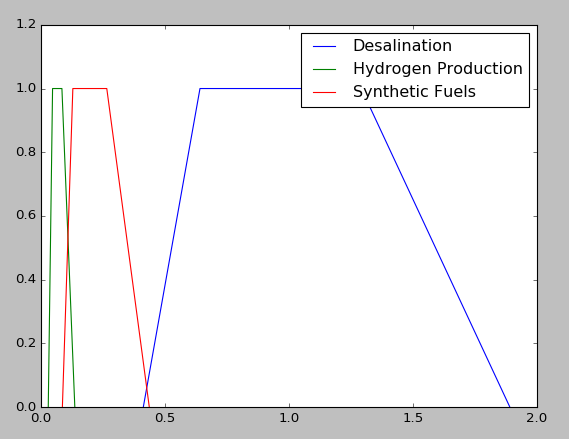
\includegraphics[width=0.5\textwidth]{membership.PNG}
  \caption{A figure displaying the fuzzy utility function for the three industrial processes.  The furthest to the right has the highest importance. Clearly Desalination has the greatest fuzzy number.}
\end{figure}


\begin{table}[h!]
\centering
\caption{AHP Survey answers for determining the relative importance of different criteria}
\label{AHPAnswers}
\begin{tabular}{|l|l|l|l|l|l|}
\hline
\begin{tabular}[c]{@{}l@{}}Pairwise \\ Criteria\end{tabular}                       & 1st Expert       & 2nd Expert       & 3rd Expert & 4th Expert       & 5th Expert       \\ \hline
\begin{tabular}[c]{@{}l@{}}Safety vs \\ Ability to \\ Fluctuate\end{tabular}       & Safety: 6        & Safety: 9        & Safety: 8  & Safety: 6        & Safety: 7        \\ \hline
\begin{tabular}[c]{@{}l@{}}Safety vs \\ Profitability\end{tabular}                 & Safety: 8        & Safety: 8        & Safety: 8  & Equal            & Safety: 7        \\ \hline
\begin{tabular}[c]{@{}l@{}}Ability to \\ Fluctuate\\ vs Profitability\end{tabular} & Profitability: 8 & Profitability: 7 & Equal      & Profitability: 8 & Profitability: 4 \\ \hline
\end{tabular}
\end{table}

\newpage
\section{AHP Conclusion and Future Work}

AHP should be used early in the design and decision making process to determine the best options given a set of criteria. Unlike other systems which can be compared to experimental setups, AHP evaluates systems which cannot have large scale experiments. Given the criteria of safety, ability to fluctuate, and profitability a multi-stage flash distillation system appears to be the best choice in a generic setup when compared with synthetic fuels upgrading and hydrogen production from high temperature steam electrolysis. In future work applying AHP to NRHES configurations, considerations such as access to feedstocks, for example water and hydrocarbons, will likely play a large role in determining the industrial process incorporated.

 Future work on applying AHP to NRHES would include many more criteria, subcriteria, and alternatives which are important to evaluate on a relative basis.  Criteria such as emissions, a key driver for NRHES, would be important to consider before determining the optimal industrial process for a given industrial park. Other criteria such as likely regulatory barriers and state of development of the industrial process technology would also be valuable to include in future research.
 



\chapter{Thermal Versus Electrical Coupling}
\label{TvsE}
Two primary motivations drive the exergy analysis described below.  The primary motivation behind this research is to demonstrate the differences in revenue generated between thermally and electrically coupling water purification systems to nuclear power plants in a \ac{nrhes} configuration.   An additional motivation is \ac{aps}, which owns about 29\% of \ac{pvgs} as well as operates the power plant, is evaluating electrically coupling a reverse osmosis system.  The \ac{ro} system will allow Palo Verde to vary the amount of electricity sent to the electric grid while generating water to meet the power plant's own water requirements in addition to increasing the water resources available for communities in the surrounding region.

Due to a high penetration of solar energy, Arizona is an ideal setting to examine the possibilities of a \ac{nrhes}. Arizona has been a leader in implementing solar electricity. In 2013, Arizona produced 23.4\% of all US solar generation and 1.9\% of the electricity within the state.  By 2016, solar in Arizona nearly doubled production to 3.4\% of the total electricity for the state. The state also has a renewable portfolio standard requiring 15\% renewable energy by 2025 from regulated utilities\cite{DSIRE2017}, including \ac{aps}. With an increasing penetration of solar in the state, other sources of generation will have to operate more flexibly to account for the variable generation. Furthermore, when California produces more electricity than that state demands, much of the overproduction is sent to Arizona either for free or California pays Arizona to take the overproduction \cite{Penn2017}. The overproduction of electricity by variable sources is only likely to increase with the California Legislature's mandate that half of the state's electricity come from renewable sources by 2030 \cite{Penn2017} and Arizona's ballot measure to raise the states renewable energy standard to demand 50\% of utility electricity come from renewables by 2030 \cite{Ballotpedia2018}.

\ac{pvgs} generates more electricity than any other power plant in the entire United States. In January 2018, Palo Verde produced 36.37\% of Arizona's power \cite{eia2018}.  As such a large contributor to the Arizona grid, Palo Verde fluctuating could counterbalance the large shifts in solar power generated during the day and unavailable during the evening and night hours. The motivation for \ac{pvgs} is to ensure the plant is not loosing money by selling electricity for less then it costs the plant to generate during certain times in the day. Palo Verde has a zero discharge water cycle.  Zero discharge means that, unlike most nuclear power plants that release heated water into a body of water, all of the water at Palo Verde either stays at the power plant forever or is evaporated from the evaporation ponds or the cooling towers.  The power plant uses waste water from Phoenix's 91st avenue treatment facility and Tolleson's water treatment facility. At the time of Palo Verde's initial operation in 1986, the treated waste water was not worth very much, but with the increasing unavailability of water and population growth in Arizona, water has become more valuable \cite{Brown2018}.  Arizona has significant amounts of brackish groundwater that could be pumped up from underground aquifers and used in place of the treated waste water currently in use at Palo Verde. The general composition of Arizona's brackish groundwater can be seen in Table \ref{ArizonaWater}.

\begin{table}[h!]
\centering
\caption{The Components of Brackish Groundwater in Central Arizona Centerra Well from \cite{USBureauofReclamation2006}}
\label{ArizonaWater}
\begin{tabular}{|l|l|}
\hline
\textbf{Material}                                                & \textbf{Mole Percent} \\ \hline
Calcium  & 7.32E-3     \\ \hline
Magnesium & 5.11E-3      \\ \hline
Sodium & 3.24E-2\\ \hline
Sulfate & 9.47E-3 \\ \hline
Barium & 5.25E-6 \\ \hline
Nitrate & 5.20E-4 \\ \hline
Flouride & 6.64E-5 \\ \hline
Arsenic & 7.21E-8 \\ \hline
Water                                                      & 99.9         \\ \hline
\end{tabular}
\end{table}

Palo Verde is pursuing a water purification facility in order to ensure a reliable and cost effective source of water for the power plant while also providing the surrounding communities with sufficient water to sustain growth. While Palo Verde is planning an electrically coupled reverse osmosis system, it is worth knowing what kind of water output would be expected from a thermally coupled system for future plants interested in pursuing desalination and water purification. Furthermore, it provides an initial model and point of reference for determining the benefits of thermally coupling as compared to electrically coupling water purification systems. Having seven separate owners has led Palo Verde in the direction of an electrically coupled \ac{ro} system, as discussed below. Since APS owns about 29.1\% of the facility, it owns about 29.1\% of the load generated from the facility. \ac{aps} has a total entitlement of about 1146 MW from Palo Verde \cite{PinnacleWestCapitalCorporation2016}. APS can allocate the electrical load it owns as desired to the \ac{ro} system in order to flexibly operate the electric load it sells to the grid as well as to ensure lower costs of water for the power plant. Even if using waste heat, thermal coupling to a reactor would impact the power cycle of the plant, as discussed in the results.  Thermally coupling any industrial process to a nuclear power plant, will require changes in the power cycle.  To have sufficient heat for even a low temperature process, some heat will have to be taken away from power generation. To avoid the complications of determining the technical as well as policy implications of thermally coupling with six owners, APS is opting for simplicity by pursuing an exclusively electrically coupled system \cite{Brown2018}.

This analysis will focus on three major benefits of coupling Palo Verde to a water purification system.  One of the primary benefits is load following by sending excess power at times when electricity is cheap to produce clean water. Second, the system can optimally use the heat produced by the reactor to produce the greatest revenue. Finally, by \ac{aps} owning the means of water production, the cost of water would be easier to predict and reliable.

The literature review presented at the beginning of this thesis revealed a notable gap in the current research modeling the benefits gained from thermally coupling compared to electrically coupling industrial processes. Thermal coupling refers to using the heat directly from the \ac{npp} in industrial processes as opposed to generating electricity, which is then used by industrial processes. Fully determining the benefits of thermal coupling requires complicated analyses that are beyond the scope of this research. The full answer requires research focused on particular projects including economic, technical, as well as political and cultural factors. The goal for this research is to address some of the possible thermodynamic and economic benefits of thermally coupling nuclear power to a water purification system at a high level focusing strictly on revenue.

The major drawbacks of thermally coupling any industrial process to a \ac{npp} are the increase in system complexity and the lack of experience in the domain. While there are cases of thermal coupling of nuclear power plants internationally, in Norway, Switzerland, Germany, and Canada \cite{Verfondern},  nuclear thermal couplings are as of yet undeveloped in the United States.  The low state of development as well as the lack of experimental data in the United States has created a lack of data and maturity of experience as a base for building such systems.  The uncertain regulatory environment regarding thermally coupled \ac{nrhess} and whether they fall under the \ac{nrc}'s umbrella also discourages development.

The success of thermally coupled systems requires that their efficiency benefits be greater than the costs associated with developing and operating thermal coupling nuclear generation and co-locating industrial processes.  An exergy analysis of both the electrically coupled and thermally coupled industrial processes provides a quantitative measure of the thermodynamic benefits of thermally coupling. The fuzzy AHP analysis concluded that, given the characteristics of safety, flexibility, and profitability, the optimal industrial process is desalination. Based on this analysis, the exergy evaluation will focus on two desalination systems.  The thermally coupled system in this analysis is \ac{msf} distillation, which will be compared to an electrically coupled \ac{ro} system. The research concludes that, while thermally coupling is thermodynamically better, electrically coupling has significant benefits in terms of flexibility, modularity, and is fairly close in thermodynamic exergy values when not much water is required.

\section{Exergy Analysis Background}
The concept of exergy is helpful for analyzing the energy allocation in a system. Exergy, also known as availability, describes the energy available in the system for doing work. Exergy has the same units as energy, most commonly Joules. Exergy destruction occurs when energy is either used for doing work or through inefficiencies in the system.  By evaluating where exergy is destroyed and the economic value the product of the exergy destruction, in this case either electricity or clean water, a hybrid energy system can be optimized for revenue. An exergy analysis can identify available exergy that used to be released into the environment that could instead be used to do the work required in a water purification system.

Exergy describes the useful energy in a system for generating work. The first and second laws of thermodynamics clarify that not all the energy generated in a system can be converted into usable work.  The first law describes how energy cannot be created or destroyed, it can only be converted into a different form.  For example, chemical combustion in a fire produces heat and light. The second law states that entropy can only increase in a system. Entropy is often thought of as the amount of randomness in a system.  Having disorder or randomness in a system requires energy that cannot be used to generate work. The entropy of a system is the energy used in the system working towards reaching a state of equilibrium.  For example, assuming a system is a room at 70\degree F with a glass of ice in it, some energy will go towards bringing the glass to the same temperature as the surrounding environment. This energy is called the entropy in the system. Some energy always goes towards the entropy in the system, making it unusable, for example, to produce electricity.


Exergy can be a more descriptive metric than energy loss as it describes how close a system is to an ideal design with the least physical possible energy losses across the system. In order to determine the maximum possible energy efficiency of a power cycle requires finding the Carnot efficiency $\eta_{Carnot}=1-\frac{T_0}{T}$. The Carnot efficiency describes the maximum possible output of a system. It is physically impossible for the Carnot efficiency to equal 100\%.  Anything above the Carnot efficiency of a cycle, which is the ideal theoretic output of a system, which would be a perpetual motion machine.  Systems will always lose energy through entropy. The exergy efficiency describes how much of the energy available to do work is transferred by the system into useful work or how effective the cycle is designed to extract all of the available energy. The exergy analysis in this research evaluates the exergy lost in the power cycle as well as the exergy lost when using the pumps. The exergy analysis can then be combined with an economic analysis determining when the greatest value is generated for each unit of exergy destroyed. For this project, the exergy analysis will include the components modeled in Palo Verde's Rankine Power Cycle as well as the water purification systems.

In an ideal reversible process, no exergy would be lost or entropy generated. Reversible processes are ideal processes that can restore the system to its initial state when the process is reversed without any external energy added to the system. No processes are fully reversible in reality. Irreversible processes increase the entropy in the system, thereby removing some of the exergy in the system. Finding where exergy is destroyed in a system can help indicate where losses are occurring. By applying an economic exergy analysis, the system can be optimized so that the exergy losses are incurred in the most valuable way possible.

The basic mass exergy equation of a system is \cite{moran2010fundamentals}:

\begin{equation}
\triangle X=(U-U_0)+p_0(V-V_0)-T_0(S-S_0)+KE+PE
\label{Xergy}
\end{equation}
\\
Where $\triangle X$ is the change in the exergy of the system from the exergy reference environment in kJ.  Exergy is rarely based off of a state of 0 K, but is instead a reference value as compared to some environment from which it differs. $U$ is the internal energy of the system and $U_0$ is the reference internal energy of the system both in kJ. $p_0$ is the reference pressure of the system in kPa, $V$ is the volume of the system and $V_0$ is the volume of the reference environment both in $m^3$. $T_0$ is the reference environment temperature given in K, $S$ is the entropy of the system and $S_0$ is the entropy of the reference environment in $\frac{kJ}{K}$. $KE$ is the kinetic energy of the system in kJ equal to $\frac{1}{2}m*v^2$ where $m$ is mass and $v$ is the velocity of the system. $PE$ is the potential energy in kJ equal to $mgh$ where $g$ is the gravitational constant and $h$ is the height of the system. The specific exergy of the system, or the exergy of the system not including the mass, is displayed as $x$.  To find the specific exergy of the system, each of the elements in the equation are divided by the mass, which is in kg in this case. Specific thermodynamic properties differ from mass thermodynamic properties in that the specific values are characteristics of the materials regardless of mass. The resulting equation for internal exergy is:

\begin{equation}
\label{specificX}
\triangle x=(u-u_0)+p_0(v-v_0)-T_0(s-s_0)+\frac{1}{2}v^2+gh
\end{equation}
\\

The elements now represent the specific values of the system with the same units as above but per unit mass as opposed to the mass dependent variables shown in equation \ref{Xergy}.  For this research, the mass based values will be neglected, focusing instead specifically on the internal exergy values. The internal exergy differences thoroughly describe the system.  The mass transfer within either the power cycle or the water purification systems does not provide any extra insight into the relative magnitude of exergy loss in the various components. The kinetic energy term, $\frac{1}{2}v^2$, is negligible due to the relatively low velocity of the system making the $KE$ small compared to the other terms in the equation thus ignorable.  The potential energy element, $gh$, is negligible throughout the system. The enthalpy, $h$, of a system, or the total heat content of the system, is equivalent to the specific internal energy plus the pressure multiplied by the change in specific volume.  Put mathematically:

\begin{equation}
\triangle h=(u-u_0)+p_0(v-v_0)
\end{equation} Including enthalpy in place of the first two elements in equation \ref{specificX} as well as removing the last two elements leaves the specific exergy equation, which is applied in this research, as simply:

\begin{equation}
\triangle x=(h-h_0)-T_0(s-s_0)
\end{equation}

\subsection{Relevant Exergy Analysis Research}
Boldon et al. have already performed an initial exergy analysis on a \ac{nrhes}, assuming a SMR \cite{Boldon}. Boldon et al. discuss the value of combining exergy and economics to analyze costs associated with exergetic losses. The assumptions in the Boldon et al. paper include a steady state system with a constant grid output of 245 MWe.  The nuclear plant is both thermally and electrically coupled to a High Temperature Steam Electrolysis industrial process. After performing the thermodynamic exergy analysis, Boldon et al. incorporate costs of resources and operations, enabling them to assign an exergetic unit cost to each of the components in the system.

The exergy analysis in this paper differs from Bolden et al. by analyzing an existing large nuclear power plant, focusing on water purification methods, including a quasi dynamic analysis, and, most importantly, focusing on revenues as opposed to costs.  An exergoeconomic cost analysis can provide relevant information to determining the price of the products generated, but it does not include the known values for the price of the products. The revenue derived from the products of the system will dictate the \$/exergy as opposed to the costs of the system.

%In order to include a quasi dynamic approach, both the MSF and RO systems are evaluated on the optimal \$/exergy costs and will also take into consideration the load following capabilities valuable to \ac{aps} through determining at what price for water and electricity it would be valuable to switch to generating water.

An exergetic analysis of the Kalundborg industrial ecosystem, a non nuclear hybrid energy system, evaluates the streams going into and out of the Asnaes power plant \cite{Valero2012}.  Valero et al. contrast the exergy of the coupled system with an uncoupled system. As can be seen in figure \ref{Kalendburg}, the Kalundborg industrial ecosystem is comprised of the Statoil refinery, the Asnaes coal power plant, the Novo Group pharmaceutical company, district heating for local residents, the Gyproc plasterboard manufacturer, as well as a fish farm and the Aalborg Portland cement company. The major exergetic gains for the system come from sharing process heat from the natural gas from the refinery, district heating, heating the fish farm, and using clinker (a coal plant byproduct) to produce cement \cite{Valero2012}. The overall reduction in irreversibilities annually from coupling the systems at Kalundborg amounts to approximately 1476 GWh/year, the equivalent of the annual production of a 170.235 MW power plant. By comparing the exergy of a coupled system with the separate industrial processes, the Kalundborg example provides insight into the thermodynamic and economic benefits of co-locating processes. Figure \ref{Kalendburg} displays the two different approaches taken; first evaluating the exergy of the combined systems, then evaluating the separate processes.

\begin{figure*}
\centering
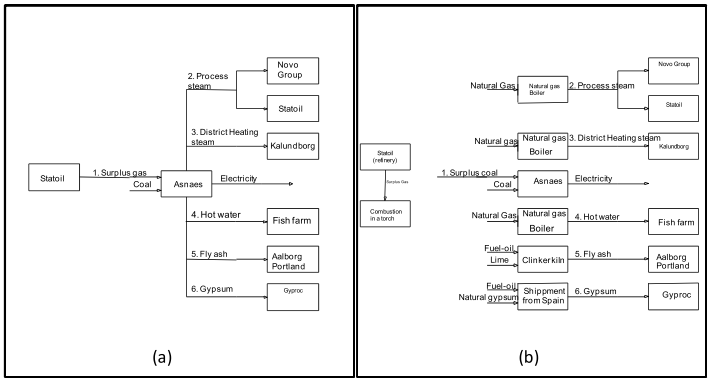
\includegraphics[width=\textwidth]{kalundborg_cases.PNG}
\caption{\small \sl This figure displays the two cases evaluated in Valero et al.: (a) shows the industrial ecosystem in the current coupled form and (b) shows the second case where there is no coupling.}
\label{Kalendburg}
\end{figure*}


\subsection{Multi-Stage Flash Distillation}
As the \ac{nrhess} evaluated for this thesis includes a \ac{msf} distillation system, a brief review of a MSF distillation exergy analysis is included. Kahraman et al. performed an exergy analysis on a large MSF plant \cite{Kahraman2005}.  \ac{msf} distillation requires heat ranging from 80 to 120 degrees Celsius, making it possible to use high temperature waste heat from a nuclear power plant to desalinate or purify the water. In general, the waste heat coming from a nuclear power plant is significantly below 100\degree C. Extra heat would thus need to be sent to the environment, in this case the MSF process, in order for the waste heat to fully power the MSF process. The same processes, RO and MSF, can be used for both water purification and desalination, so the terms can be used fairly interchangeably. In the case of Palo Verde, the system is a water purification system for brackish groundwater. In the exergy analysis, Kahraman et al. takes the temperature of the salinated water to be the assumed reference environmental conditions for the system, making the initial exergy zero. Similarly, in the exergy performed in this thesis, the assumed reference environmental conditions are taken as the temperature of the water intake. Kahraman et al.'s exergy analysis includes finding the exergy of the heat exchanger and four pumps in the system, as well as calculating the difference in exergies between the incoming water and the exiting pure water. The analysis is used to find the overall exergy efficiency and determine where to reduce exergy destruction in the system.

Figure \ref{MSF_x} displays where exergy is destroyed in the MSF system. Clearly the majority (77.7\%) of the exergy is destroyed in the MSF distillation system itself. Other sources of irreversibilities include the inefficiencies and losses due to the pumps and heat exchangers as well as the final release of the waste brine water to the environment. The exergy destroyed in the MSF system went to a process that produced a valuable product.  The other sources of exergy destruction are physically necessary losses with no economic benefits. In the economic exergy study performed in this thesis, the exergy destruction will be evaluated based on its economic value.  Both generating pure water in the MSF system as well as producing and using electricity for the reverse osmosis system result in exergy destruction.

\begin{figure*}[h!]
\centering
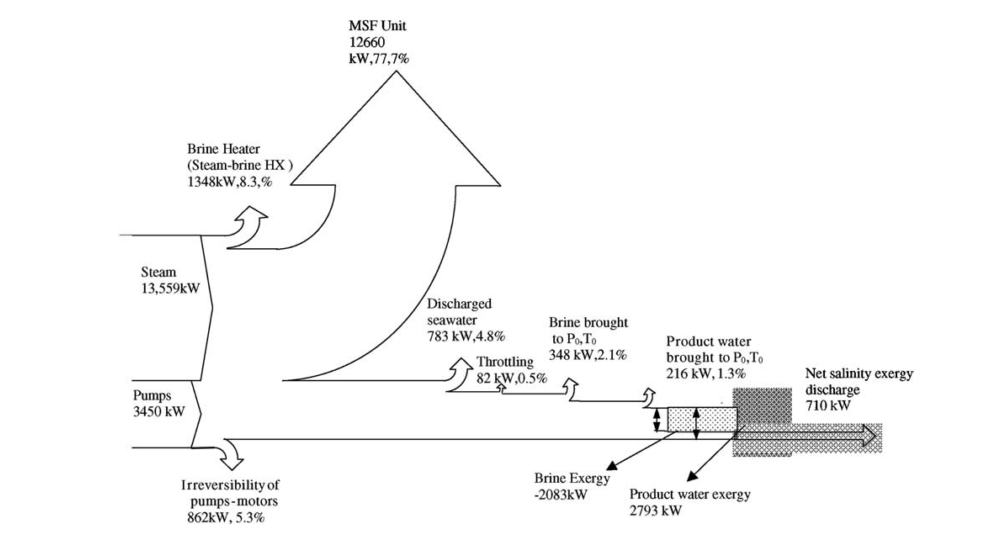
\includegraphics[width=\textwidth]{MSF_exergy.PNG}
\caption{\small \sl The Multi-Stage Flash exergy analysis diagram showing where exergy is lost in the system.  This exergy diagram was published in \cite{Kahraman2005}}.
\centering
\label{MSF_x}
\end{figure*}

MSF is a common thermal desalination system, making up about 21\% of the total worldwide installed capacity as can be seen in figure \ref{DesalData}. In an MSF system, salt water or brackish water is flash evaporated, then condensed repeatedly in order to remove unwanted particulates. As can be seen in figure \ref{salinity}, brackish water has more salinity or impurities than fresh water, but not as much as sea water. MSF can produce clean water in large quantities, with plants in Saudi Arabia and the United Arab Emirates having capacities of 600,000-880,000 $m^3/day$ \cite{El-Dessouky2016}. In general, an MSF system works by passing sea water or brackish water through a series of chambers, each with successively lower temperature and pressure.  The water is quickly flashed, or vaporized.  The water, without the brine, is then condensed, forming freshwater.  The stages can range widely, depending on the concentration of the feedwater brine and the desired state of purity for the freshwater. Standard sizes for fairly large MSF arrays range from 21 to 50 stages. Generally, MSF distillation systems are a well-developed technology used for high capacity desalination systems.
\begin{figure*}[h!]
\centering
\label{DesalData}
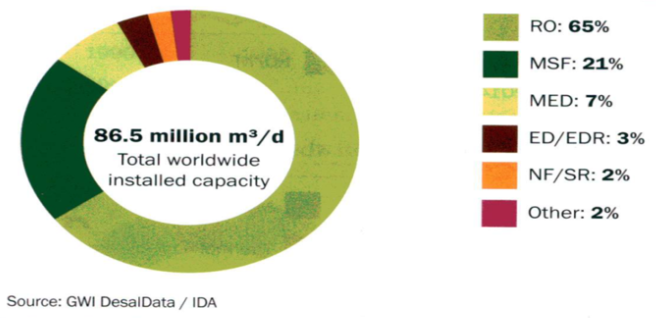
\includegraphics[width=\textwidth]{DesalData.PNG}
\caption{\small \sl This pie chart from \cite{Khamis} shows the overall total installed capacities of each of the technologies used for desalination. The six technologies shown represent Reverse Osmosis (RO), Multistage Flash (MSF), Multiple-effect distillation (MED), Electrodialysis Reversal (ED/EDR), and Nanofiltration (NF)}
\centering
\label{DesalData}
\end{figure*}



\begin{figure*}[h!]
\centering
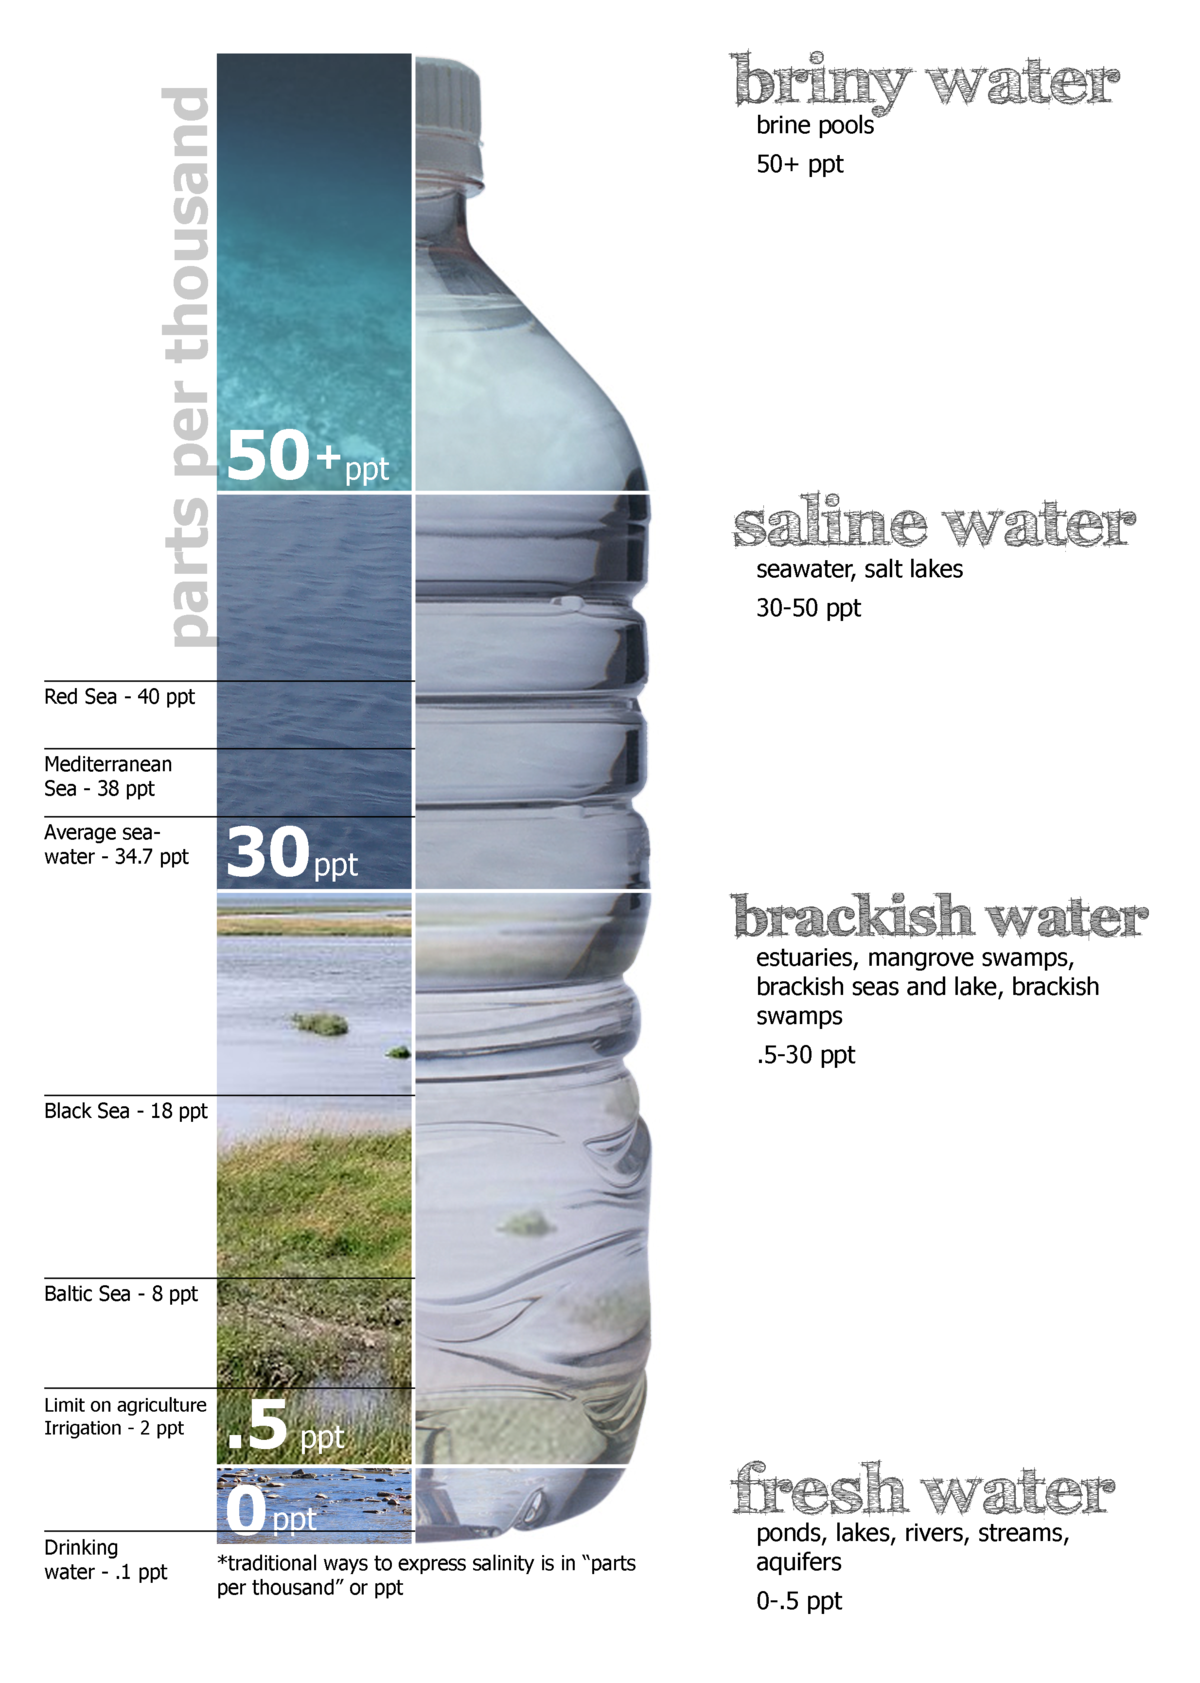
\includegraphics[width=.5\textwidth]{Water_salinity_diagram.png}
\caption{\small \sl This figure displays the differences between different water qualities.  The groundwater in Arizona qualifies as brackish \cite{USBureauofReclamation2006}.  This image is from \cite{Summerlin}}
\label{salinity}
\end{figure*}


In a multi-stage flash system, it is important to keep the temperature relatively low, no greater than 120 \degree C, in order to minimize fouling. Fouling and scaling are serious considerations for MSF systems.  Generally, fouling refers to the unwanted deposition of compounds or organic substances on the surface of a host material (membrane, heat exchanger, condenser, etc)\cite{Khayet2016}. Scaling is when a surface is entirely covered with a mineral film coating. In \cite{El-Dessouky2016} the twelve case studies range from 95 \degree C to 105 \degree C. For a more complete range of possible temperatures, this research will analyze temperatures from 80 \degree C to 120 \degree C. The largest MSF plant produces about $91,000\frac{m^3}{day}$.




\subsection{Reverse Osmosis}

Reverse osmosis is a type of electrically driven membrane desalination or filtration process. It can remove tiny particles of sizes ranging down to 50-200 daltons \cite{Pangarkar2011}. It has relatively high applied pressure values ranging between 1-5 MPa. In general, the reverse osmosis system works due to the osmotic pressure differences between salt water or brackish water and pure water. During the \ac{ro} process, salt water or brackish water is forced through membranes under pressure, separating the feedwater into a pure water stream and a stream with a high concentration of impurities.  Generally, about 4kWh is required for every cubic meter of clean water \cite{Pangarkar2011}. About 48\% of reverse osmosis systems are used with brackish water \cite{Pangarkar2011}. The largest sea water reverse osmosis desalination plant in the world is in Israel and produces about $624,000\frac{m^3}{day}$. The amount of water produced by the RO facilities in this study is significantly greater than the output of the largest facility in the world.  The goal for this research is to determine the relative potential outputs of the various configurations, not the realistic values.

%Should probably remove the last pump since it uses 1.58 kwh/m^3



\section{Methodology}
 The exergy analysis performed here will assume a simplified model of the Palo Verde Rankine power cycle, seen in figure \ref{basePC}, and compare a process heat MSF distillation system to a RO system.  First, the  \$/exergy cost of an MSF system will be evaluated using the process heat from a nuclear power plant. Then the same process will be applied to the exergy costs of the RO system, which strictly uses electricity. Traditionally an economic exergy analysis, also known as an exergonomic or thermoeconomic analysis, evaluates the most costly exergy losses in a system. In this case each of the components in the power cycle and industrial process would be evaluated based on their capital and maintenance costs as well as the specific exergy losses associated with the process.  This is commonly referred to as the \ac{speco} approach.  In this case, the motivation behind coupling with an industrial process is not minimizing the costs of generation, but instead optimizing the profit.  Evaluating the economics of the exergy losses associated with each of the components of the system does not answer the fundamental question of which system will generate the greatest profit given a fluctuating price for electricity and ever increasing price for water. The exergy losses in the RO system comes from the exergy destroyed in the pumps and is added to the exergy loss required to generate the electricity. The economic values for the system will come from the value of the electricity generated plus the value of the water generated. While the exergy analysis performedin this research does not include the capital, operations, and maintenance costs of the two systems, it does suggest what the differences are likely to be between the two systems.  It does so by demonstrating how each pump added to the RO system reduces the overall revenue per unit of exergy.

 \begin{figure*}[h!]
\centering
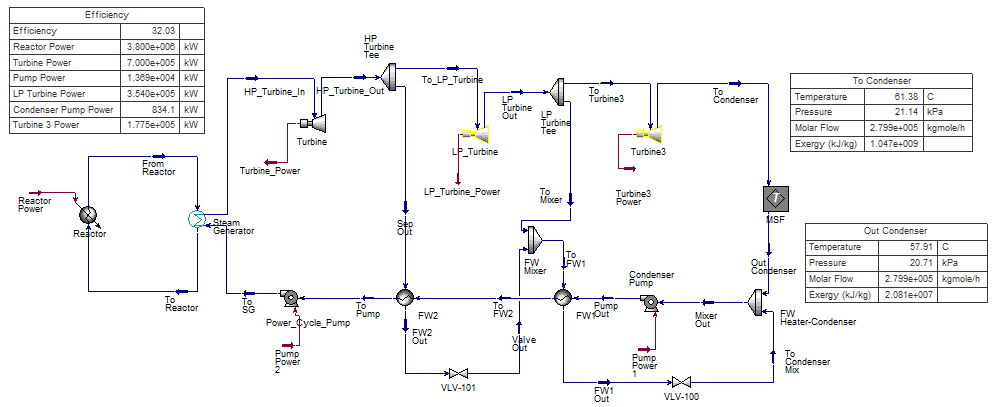
\includegraphics[width=\textwidth]{ActualPC.PNG}
\caption{\small \sl Palo Verde's simplified Rankine cycle used for this research. The overall efficiency of the system is about 32\%, which is a reasonable approximation of the Palo Verde Power cycle.  The turbines are yellow, meaning warning, because of the liquid entering the turbines.  In reality, the turbines can still function with some liquid}
 \label{basePC}
\centering
\end{figure*}

A simplified model of the \ac{pvgs} power cycle is constructed using Aspen HYSYS.  Since the goal in this research is to evaluate the differences in the water purification systems, not the exergy losses in the power cycle, the power cycle model primarily serves to demonstrate how thermally coupling a system impacts the system as a whole. While a more precise model of the \ac{pvgs} would provide more precise results, the goal of this project is to show the relative benefits of multiple water purification approaches. The overall exergy lost is the same throughout the power cycle; the losses can generate either electricity or water.

\subsection{Aspen HYSYS}

Aspen HYSYS is process simulation software used primarily by the oil and gas industry. In general, process simulation software calculates material and energy balances for a whole plant or process unit. Process simulation software can be used to size the various components in a system for the desired outcome in terms of quality and quantity of product. Aspen HYSYS calculates heat and mass balances, thermodynamic data and equilibrium conditions, sizes equipment, and can do economic optimization and dynamic simulation \cite{Oi2017}. In this model, Aspen HYSYS calculates the overall thermodynamic and mass flow values of the Palo Verde power cycle as well as the multistage flash distillation process. The thermodynamic values, such as enthalpy, entropy, temperature, and pressure can then be used to determine the exergy of the system using a User Variable in the system.

First, as can be seen in figure \ref{basePC}, determining the exergy analysis required initially building the Palo Verde power cycle using Aspen HYSYS and then coupling it to both a MSF and RO water purification systems. The configurations for the MSF and RO systems can be seen in figures \ref{MSF} and \ref{RO} respectively. After the building the model, in order to find  the \$/exergy in the power cycle and the water purification system required using a combination of user variables within Aspen HYSYS as well as spreadsheet calculations, as can be seen in Appendix B. Then, after finding the exergy values, in order to determine the optimal temperature of water required adjusting the temperature of the water sent to the heat exchanger with the MSF system.

\begin{figure*}[h!]
\centering
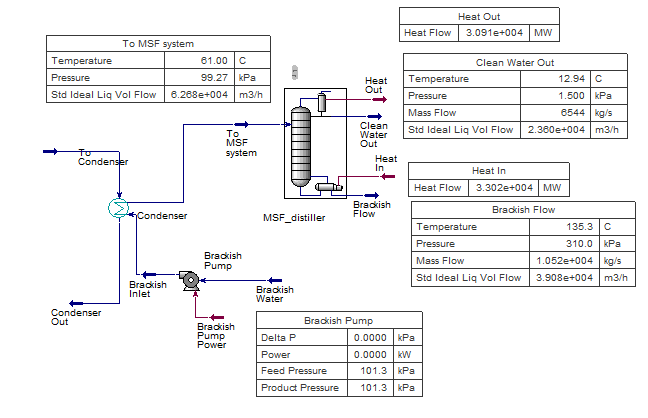
\includegraphics[width=\textwidth]{PowerCycle.PNG}
\caption{\small \sl The distillation column used to represent the multi-stage flash system along with key important metrics for the various components.}
\label{MSF}
\centering
\end{figure*}

\begin{figure*}[h!]
\centering
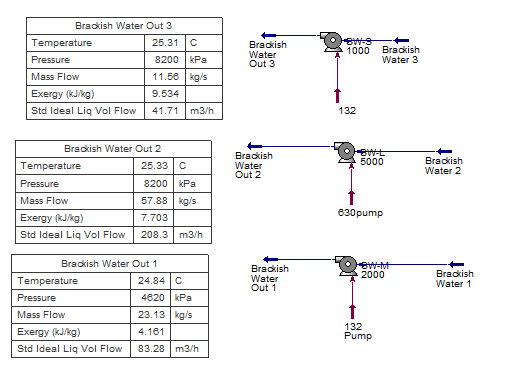
\includegraphics[width=\textwidth]{ROimage.PNG}
\caption{\small \sl The energy used for an RO system is directed almost entirely to the pumps used.  The three pumps shown here represent off-the-shelf pumps used in Reverse Osmosis systems}
\label{RO}
\centering
\end{figure*}

Doing an economic analysis evaluating the \$/exergy requires knowing the amount of product sold as well as the value of the product. The cost of water for Palo Verde in 2018 is \$130.00 per acre-foot, which comes out to about \$0.105 per cubic meter of water \cite{Brown2018}. The water Palo Verde consumes is cheap compared to the residential cost of water in Tucson which was about \$1.42 per cubic meter in 2017\cite{CityofTucson2017}. The best value available for the wholesale value of Palo Verde's electricity is from 2007 at 6.33 cents per kWh, which is equal to about 8 cents per kWh in 2018 dollars including inflation over the past 11 years. The actual value of the electricity varies over a day depending on the supply of electricity and grid demand. The highest wholesale price paid per MWh in the Palo Verde Southwest price hub was \$165.  The lowest wholesale price paid per MWh in the Palo Verde Southwest price hub was \$13.50 \cite{EIA2017}.  The \$80 per MWh price assumed in this research is on the high side, but still within the range.  The actual wholesale price of electricity for Palo Verde is confidential information, so the price values are approximations.  In Arizona's case, the value of the electricity over the course of a day is largely influenced by the amount of solar supply available to the grid from both Arizona and California. The fluctuation in power demand for \ac{aps} will be taken into consideration using \ac{raven} to generate demand data for a generic day in each season.

\subsection{Fluctuating Electricity Output}

The definition of a regulating and supplemental reserve of electricity differs depending on the region and \ac{iso} \ac{nerc}.  The Independent Electricity System Operator (IESO), which manages most of Ontario, Canada's grid maintains that spinning reserve, such as nuclear plants, to be considered operating reserve or 10-minute spinning must make energy available within 10 minutes of the contingency so that the supply matches the demand\cite{NERC2014}. NPPs traditionally are unable to fulfill a role as regulating or supplemental reserve because of the inability to ramp to full power quickly.  With an MSF system, the NPP still may be unable to switch the process heat fast enough to meet the IESO's definition. The European Utility Requirements require that an NPP be capable of daily load cycling operation between 50\% and 100\%. The European pressurized water reactor must satisfy maneuverability requirements, including being able to have planned variations in energy output between 25\% and 100\% \cite{NEA2011}. For this research, the MSF process heat model will be evaluated at 25\%, 50\%, 75\%, and 100\% of the heat load from the reactor. Looking at 25\% intervals will give some notion of the relationship between the heat sent to the MSF system and the amount of water collected from the system.

There are several nuclear power plants which are already manipulating the amount of load they send to the grid.  Energy Northwest is reducing the amount of load it sends to the grid to 80\% of capacity when there is too much electricity on the grid and the price of electricity is low.  Duke Energy is currently evaluating how to reduce their nuclear output to the grid, also establishing a minimum of 80\% of rated capacity \cite{siphers}.  Since the standards are significantly different in the United States as compared to Europe, smaller fluctuations ranging from between 5\% and 20\% will also be evaluated for each of the cases.

\subsection{Drinking Water Standards}
Water quality standards must be met to ensure the water produced by the purification process is of high enough quality to use in Palo Verde's power cycle as well as to sell to the public. The main consideration for the water purification system, especially if the water is planned for sale to the public, is that the water must meet the standards established by the Safe Drinking Water Act of 1974. While commercial nuclear power plants dedicate a lot of resources to water chemistry and have very high standards for the water used in the plant, the standard used for this research will be that set for public consumption. The Safe Drinking Water Act of 1974 gives the \ac{epa} the authority to determine drinking water standards. The EPA sets standards on over ninety contaminants in drinking water. The drinking water contaminants fall into the broad categories of microorganisms, disinfection byproducts, disinfectants, inorganic chemicals, organic chemicals, and radionuclides \cite{USEPA}. The make up of Arizona groundwater can be found in table \ref{ArizonaWater}.  None of the contaminants found in Arizona groundwater are regulated by the Safe Drinking Water Act or are covered by the EPA's secondary drinking water standards \cite{USEPA}. The only overlap between the contaminants regulated by the EPA for taste and aesthetic concerns and those found in Arizona groundwater is maintaining the total dissolved solids at 500 mg/L or below. For this research, the water is assumed to be comprised of a more brackish composition than that found in table \ref{ArizonaWater}. The contaminants have been increased nine fold in the composition used in the Aspen HYSYS model, as can be seen in table \ref{ModelComp}.  In some cases, the independent materials found in the brackish ground water were unavailable in the Aspen library.  As a result, the model includes combined molecules, such as sodium sulfate and sodium nitrate to most closely proportionally match the composition found in the groundwater.  Combining these molecules may result in some difference in the overall composition and the energy it takes to remove the particulates. The end product is clean water, with the model composition displaying 100\% water.

\begin{table}[h!]
\centering
\caption{Mole Composition of Brackish Groundwater Assumed in Aspen-HYSYS model}
\begin{tabular}{|l|l|}
\hline
\multicolumn{1}{|c|}{\textbf{Material}}                   & \multicolumn{1}{c|}{\textbf{Mole Percent}} \\ \hline
Calcium & 1.3E-1 \\ \hline
Magnesium  & 9E-2\\ \hline
Sodium  & 5E-1 \\ \hline
Sodium-Sulfate & 1.7E-1 \\ \hline
Sodium-Nitrate & 9E-2 \\ \hline
Barium & 1E-2 \\ \hline
Water & 99.0  \\ \hline
\end{tabular}
\label{ModelComp}
\end{table}

\section{Palo Verde Power Cycle}

Much of the information on the design and functioning of Palo Verde's power cycle can be found in the \ac{ufsar}, as can be seen in tables \ref{coreValues} and \ref{PowerValues} made publicly available for all nuclear power plants by the \ac{nrc}. Some of the key values taken from Palo Verde's \ac{ufsar} are displayed in tables \ref{coreValues} and \ref{PowerValues}.  The second value represents the converted value into the units used in the model of this thesis.  The key difference between the model values and the Main Steam Flow Power Cycle Values is the mass flow is significantly less for the model 1616- $\frac{kg}{s}$ compared to 2200 $\frac{kg}{s}$. The mass flow value is solved for in the model. As the thermodynamic values taken for this research are specific values that do not include the mass flow, the findings should be relevant to any mass flow. Overall, while the simplified Palo Verde power cycle does not precisely model the actual power plant, it has enough similarities to suggest some trends via the exergy analysis. Since not all of the components are included in the model, the lower mass flow calculated is to be expected.

\begin{table}[h!]
\centering
\caption{Palo Verde Reactor Core Thermohydraulic Values. The first units given in the Value Given in FSAR column are the actual values found in the FSAR, while the second are the converted values into those used in the model.}

\begin{tabular}{|l|l|l|}
\hline
\textbf{Reactor Core Values} & \textbf{Value Given in FSAR} & \textbf{Value in Model}        \\ \hline
Reactor Outlet Temperature   & 653 \degree F, 345\degree C & 345 \degree C   \\ \hline
Reactor Inlet Temperature    & 568 \degree F, 297.8 \degree C &  297\degree C\\ \hline
Mass Flow                    & $164.0x10^6\frac{lb}{hr}$    & $20663.6\frac{kg}{s}$          \\ \hline
Pressure                     & 2250 psia, 15.513 MPa                    &  15.51 MPa                    \\ \hline
Power Generation             & 3990 MWt                     & 3990 MWt                       \\ \hline
\end{tabular}
\label{coreValues}
\end{table}


\begin{table}[h!]
\centering
\caption{Palo Verde Main Steam Flow Power Cycle.}
\label{PowerValues}
\begin{tabular}{|l|l|l|}
\hline
\textbf{Power Cycle Values} & \textbf{Value Given in FSAR}  & \textbf{Values in Model}          \\ \hline
Steam Temperature at HX     & 552.9 \degree F (289.4 \degree C) &   289.4 \degree C                 \\ \hline
Mass Flow                   & $17.2-18.1x10^6\frac{lb}{hr}$ ($2154.56-2280.56 \frac{kg}{sec}$) & 1616 $\frac{kg}{sec}$ \\ \hline
Pressure & 1070 psia (7.377 MPa)  &   7.377 MPa                     \\ \hline
\end{tabular}
\label{PowerValues}
\end{table}

There are two model configurations included in this analysis.  One of the configurations, as seen in figure \ref{MSF_condense},  draws water from the end of the power cycle.  As the Palo Verde Power Plant would want to minimize impact to the thermal hydraulics of the system, using the condenser and switching to passing groundwater through the system would allow for use of existing infrastructure. The second configuration, shown in figure \ref{MSF_SG}, allows for a more efficient system that draws water straight from the steam generator at very high temperatures. Since the efficiency of the ideal Carnot cycle is very dependent on the change in temperature through the cycle, drawing water from the steam generator allows for a greater drop in temperature throughout the cycle.  When taking a percentage of the water at the beginning of the power cycle, the water leaving the last turbine does not have to be a minimum of 80\degree C for the \ac{msf} system.  Also, water at 289.4\degree C can heat a lot of water at 24.44\degree C to 80\degree C. The second configuration would allow for differing amounts of water to be sent to the MSF as opposed to different temperatures of water, as is the case when using the condenser as a heat exchanger for the MSF system.

\begin{figure*}[h!]
\centering
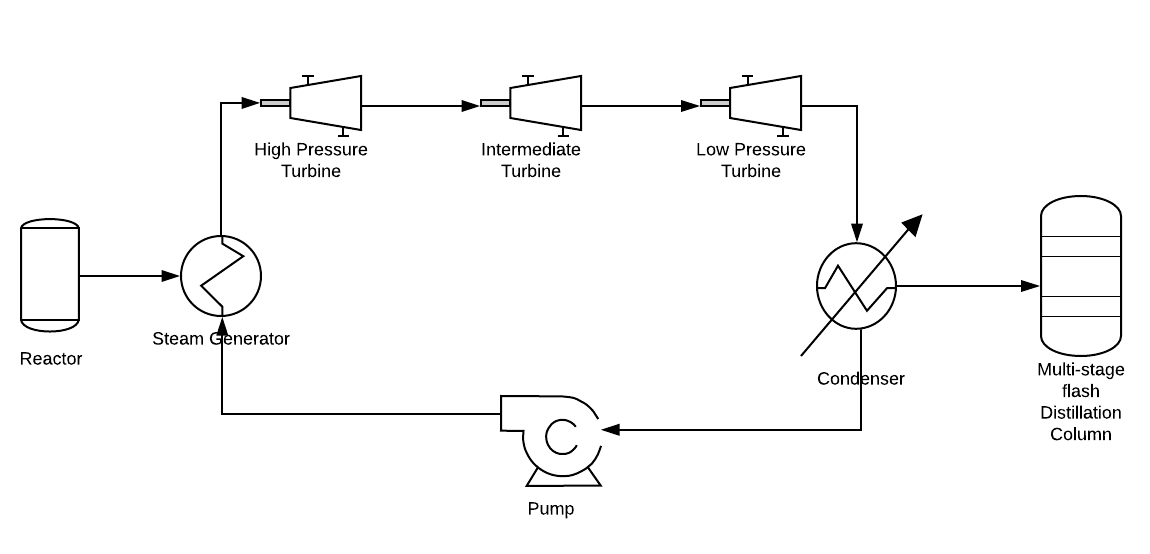
\includegraphics[width=.8\textwidth]{MSF_condense.png}
\caption{\small \sl This simplified drawing shows the main components of the power cycle including how the multistage flash distillation system is heated through the condenser}
 \label{MSF_condense}
\centering
\end{figure*}

\begin{figure*}[h!]
\centering
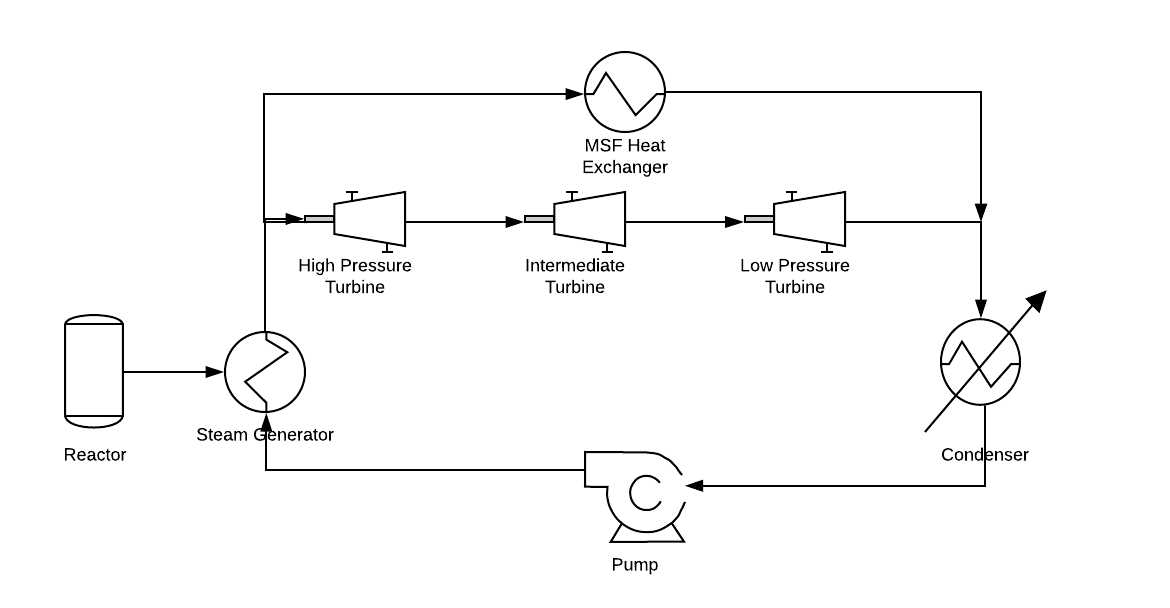
\includegraphics[width=.8\textwidth]{MSF_lucidchart.png}
\caption{\small \sl This simplified drawing shows the main components of the power cycle including how the multistage flash distillation system draws water just after the steam generator}
 \label{MSF_SG}
\centering
\end{figure*}

\clearpage



\clearpage
\subsection{Assumptions}

Given the information above, the assumptions for both the \ac{msf} and \ac{ro} Aspen HYSYS models are:
\begin{enumerate}
\item The temperature of the brackish groundwater entering the system is 76 \degree F or 24.44 \degree C, the low end of the temperature range for the water currently used to cool the system \cite{Brown2018}. Groundwater would be colder, but sitting in a pool above ground would raise the temperature. The assumption of the water being at the low end of what currently flows through the condenser allows an analysis of using the groundwater and also allows for a fair comparison of the MSF and RO systems using the most realistic value for both.
\item The reactor power, as given in the FSAR, is 3990 MWth.
\item The temperatures for the MSF distillation unit range from 80 \degree C to 120 \degree C. Since the 80\degree C water generated the most water in each circumstance, only the 80\degree C model is discussed.
\item The composition of the water is shown in \ref{ModelComp}.
\item There is a 2\% pressure drop across all heat exchangers.
\item The turbines in the Palo Verde power cycle have a 90\% adiabatic efficiency.
\item The pumps have a 90\% adiabatic efficiency.
\item The fluid package used for the power cycle is Peng-Robinson, which is the fluids package with the largest applicable range for temperature and pressure.
\item The fluid package used for the brackish water is Aspen's Electrolyte Non-Random Two-Liquid (NRTL). This fluid package is especially good for modeling all of the various components in the brackish feedwater composition.
\item The power cycle is much simplified in order to show the clear impacts of the different water purification techniques as opposed to emphasizing the power cycle itself.
\end{enumerate}

The assumptions for the MSF Aspen HYSYS models are:

\begin{enumerate}
\item There are twenty one stages in the MSF distillation system \cite{Bodalal2010}.
\item The mass flow through the distillation system is the dependent variable while the temperature of the water sent to the unit and the pressure generated from the brackish water pump are the independent variables for the MSF system.
\item The reactor power and electricity produced are independent variables.
\item The temperature of the water sent to the condenser is an independent variable.
\item The pump power is a dependent variable.
\item The electric power generated is an independent variable.
\item The amount of water generated and the electricity generated are the dependent variables depending on the desired temperature of water sent to the condenser.
\end{enumerate}

The assumptions for the RO Aspen HYSYS model are:

\begin{enumerate}
\item The efficiency of the pumps range from 70\% to 80\% depending on the specifics of the expected pressure and water outflow provided by the company, the specifics of which can be seen in Appendix \ref{Appendix:pumps}.
\end{enumerate}

The economic assumptions for all Aspen HYSYS models are:
\begin{enumerate}
\item The cost of water for Palo Verde Generating Station is \$130 per acre foot \cite{Brown2018}
\item The wholesale price which Palo Verde can sell electricity to the grid is \$.08 per kWh.
\end{enumerate}

The simplified Aspen HYSYS model includes one high pressure and two low pressure turbines.  The three separate turbines can be taken offline independently to send higher temperature water to the MSF system. The exergy analysis performed here is different than most economic exergy analyses in that it considers the revenue from each product, not the cost.  Generally, exergy analyses consider the costs of each of the various systems to see where there is the greatest cost to exergy losses.  As the prices for the various products are more readily found than the cost of generating the electricity or the steam, the revenue is evaluated here.  While a \ac{speco} approach is currently in development, one of the built-in assumptions is that the revenue associated with any given unit of exergy will be the same no matter if the heat is used to generate electricity or a secondary produce \cite{Paulus2006}.  In the case of a system that generates multiple products, such as the system evaluated in this thesis, and uses exergy that would otherwise go unused, there is a difference in the exergy value at different locations in the system. Calculation of the \$/exergy values for this analysis the following calculations were applied:

Using equation \ref{electricity}, the electricity revenue is calculated by multiplying the electricity produced by the system in MW by the wholesale electricity price per MWh, assumed here to be \$80 per MWh:
\begin{equation}
Electricity\hspace{.2cm} Revenue=MW_{out}*\frac{\$80}{MWh}=\frac{\$}{hr}
\label{electricity}
\end{equation}

The water revenue is then calculated using equation \ref{water}, which multiplies the water produced by the system by the wholesale value of water to the Palo Verde Generating Station:
\begin{equation}
Water\hspace{.2cm} Revenue=\frac{m^3_{out}}{hr}*\frac{\$.105}{m^3}=\frac{\$}{hr}
\label{water}
\end{equation}

Equation \cite{revenueX} is then applied to find the \$/exergy destroyed:

\begin{equation}
\frac{\$}{Exergy\hspace{.2cm}destroyed}=\frac{Electricity \hspace{.2cm} Revenue+ Water \hspace{.2cm} Revenue} {Total\hspace{.2cm}Exergy\hspace{.2cm}Destroyed}
\label{revenueX}
\end{equation}

For the RO system the same equations are used to generate electric and water revenues. The $\frac{\$}{exergy}$ cost for the reverse osmosis system is calculated by dividing the water revenue-cost of electricity by the exergy used across the pumps:

Using \ref{Xdestruct}, the total exergy destroyed is calculated as:

\begin{equation}
Exergy\hspace{.2cm}Destroyed = Power\hspace{.2cm}Cycle\hspace{.2cm}Exergy\hspace{.2cm}Destroyed+RO\hspace{.2cm}Pump\hspace{.2cm}Exergy\hspace{.2cm}Destroyed
\label{Xdestruct}
\end{equation}

The \$/exergy value for the RO system is:

\begin{equation}
\frac{\$}{Exergy\hspace{.2cm}Destroyed}=\frac{Electricity \hspace{.2cm} Revenue+ Water \hspace{.2cm} Revenue}{Exergy\hspace{.2cm}Destroyed}
\end{equation}

Generally, an exergy analysis evaluates the cost per unit of specific exergy.  Overall it analyzes how much is spent in generating every unit of exergy and therefore how much is worth spending to enhance the exergy efficiency through other steps, such as purchasing more efficient pumps, condensers, or turbines.  The initial exergy analysis in this research attempts to look purely at the revenue per unit of exergy.  Since the value of the electricity and water are already known, the approach of evaluating the overall revenue established an initial means of analyzing the system. The exergy analysis finds the exergy generated by the reactor and analyzes which coupled water purification design uses that exergy to generate the greatest overall revenue.  This is a simple analysis which does not include the operations, maintenance, or capital cost.  It simply determines how the exergy can be allocated to result in the greatest overall revenue.

%The results in section 3.4 demonstrate that the revenue for the system is greater with the reverse osmosis process than with the MSF system, even though the RO system had worse overall \$/exergy values in all cases, sometimes there is a significant difference. In reality, the overall revenue is not important.  The \$/exergy value differences are exaggerated when costs are included.  For the RO case, every new pump comes at a greater cost.  The cost of the system increases linearly along with the revenue value.  For the MSF system, the costs decrease as the water production increases since the cost of initial installation is the major expense.  While increases in the MSF system size result in higher costs, the overall cost per unit of exergy sent to the system would decrease. The simple approach to an exergy analysis employed in this system provides insight into that relationship.  The RO system has very similar values when not much water is generated, but significantly lower values when more water is generated.

%Once discovering that doing just a straightforward revenue analysis did not tell the total story of what is going on in these systems, a more traditional thermoeconomic exergy analysis is performed.  The major part of the story missing when looking exclusively at revenue is the incredible difference in capital costs for the two systems.  The RO system had thousands of pumps which would cost an unimaginable sum.  The MSF system, on the other hand, does not really change capital cost values.  There are the same overall number of stages no matter how much water is passing through.  The differences in capital costs are the initial costs for the materials and then of installation.  Reverse Osmosis has major costs in terms of maintanence and materials, with the need to change out the membranes on a fairly regular basis or loose a lot of efficiency in the system.

\section{Results}

The results of this study focus on answering questions about three possible beneficial areas from coupling Palo Verde to a water purification system. The benefits include 1) varying the electricity output to the grid, 2) optimizing the value of the exergy lost in the system, and 3) providing reliable and reasonably priced water to Palo Verde.  The results discussed below are organized into discussions pertaining to these three areas.


\subsection{Flexibility}
The ability of a system to operate flexibly is of growing significance and value. As APS implements the required amount of renewable generation, other generation sources will need to change their output to the grid in response. A more thorough analysis of the flexibility requirements for Palo Verde is provided in section 3.5. There is a value in sending various loads to the water purification process for different points in the day as the power needs of the grid vary. To do a parametric study of the ability for the RO system and the MSF systems to take the different amounts of load, the model is evaluated first at 5\%, 10\%, 15\%, and 20\% and then at 25\%, 50\%, 75\%, and 100\% of capacity output to the grid as discussed previously.

This thesis does not include a quantitative study of the ability of the two water purification techniques to start and stop, but the research literature makes it clear that reverse osmosis systems are easier to run in a dynamic fashion.  The MSF system requires careful maintenance between the power generation and water generation processes.  There is a small range of temperatures within which the MSF unit can operate.  If performed improperly, the MSF unit could automatically trip off \cite{Radif}.  The RO systems, being essentially a large number of pumps forcing water through membranes, are able to start and stop and produce the same quality of water.  Both systems are able to start and stop.  In the AHP analysis, desalination ranked highest in flexibility. While this is an imperfect measure, it does suggest that the flexibility is a benefit of desalination.

%The arrangement with the best overall \$/exergy value for the load following examples is the thermally coupled plant with the heat taken from the condenser.  When allocating  a 10\%  This arrangement can be more carefully controlled than taking the heat from the condenser since the amount of water split off can be determined on the fly.  The condenser example requires that the water sent through the heat exchanger is at least 80\degree C which does not allow it to reduce the load only 5\%. The scenario with the greatest overall revenue on the other hand, is the SW-L 630 kW pump.  The heat required to reduce the load 5\%  produced significantly less water in the thermally coupled system than in the reverse osmosis pump.  Due to the higher exergy costs of the pumps, the overall \$/exergy is significantly less.

Tables \ref{SGLF} through \ref{SW-L} display the overall \$/exergy values as well as how much electricity and water were generated hourly.  Each of the configurations and reverse osmosis pumps are evaluated at 5\%, 10\%, 15\%, 20\%, 25\%, 50\%, 75\%, and 100\% with the exception of the MSF system coupled at the condenser.  This configuration is unable to reduce to 5\% output due to meeting the minimum heat requirement of 80\degree C requiring more than 5\% of the energy from the power cycle. The exergy destruction in the power cycle is the exergy taken into consideration.  The tables show which system generates the most revenue for the exergy created by the reactor. The greatest overall \$/exergy value is the MSF system coupled to the reactor at the condenser at \$117.57.  This is greater than the system when all of the exergy is used to generate electricity, which has a value of about $\frac{\$100.77}{\frac{kJ}{kg}}$. The reverse osmosis systems output a greater \$/exergy value after the 10\% load follow.  The RO pumps increase output linearly while the MSF unit flattens out as more exergy is sent to the water production. Of the reverse osmosis pumps assumed, the highest revenue per unit of exergy change is from the IDE-Progreen SW-L 630 kW pump.  While the MSF unit coupled at the condenser has the greatest overall \$/exergy value, the reverse osmosis systems are greater in every other \$/exergy load following amount.  The MSF unit can generate a lot of water with lower levels of power, but the RO unit linearly outputs water.

The largest reverse osmosis plant in the world produces about $624,000 \frac{m^3}{day}$, or about $26,000\frac{m^3}{hr}$ of water. The largest MSF distillation system in the world produces approximately $92,000\frac{m^3}{day}$, or about $3800\frac{m^3}{hr}$.  The values shown in the results tables are significantly greater than the output of the largest water purification systems in the world, which is unreasonable. The number of pumps required for sending large quantities of electricity to the reverse osmosis system are not reasonable. Similarly, the size of the MSF unit would need to be enormous to use large quantities of heat from the reactor.  The reason for including the deep load following percent reduction is to show how the two systems compare based on revenue. The results are there to demonstrate the differences between the different configurations. The capital costs would be too great to build configurations sufficiently large to operate flexibly above about 5\% of one of Palo Verde's reactors.

\begin{table}[h!]
\centering
\caption{Load following outcomes using the thermally coupled MSF distillation system drawing heat directly after the steam generator at smaller interval load reductions assuming a 20\% reduction limit}
\label{SGLF}
\begin{tabular}{|l|l|l|l|l|l|l|}
\hline
\multicolumn{1}{|c|}{\textbf{\begin{tabular}[c]{@{}c@{}}Load\\  Following\\ Percent \\ Reduction\end{tabular}}} & \multicolumn{1}{c|}{\textbf{\begin{tabular}[c]{@{}c@{}}Percent \\ Water\\ Split\end{tabular}}} & \textbf{\begin{tabular}[c]{@{}l@{}}Volume\\ Flow Out\\ $\frac{m^3}{hr}$\end{tabular}} & \textbf{\begin{tabular}[c]{@{}l@{}}Power\\ MWe\end{tabular}} & \textbf{\begin{tabular}[c]{@{}l@{}}Hourly \\ Total\\ Revenue\\ (\$/hr)\end{tabular}} & \textbf{\$/exergy} \\ \hline
5\%   & 0.988   & 607.5  & 1244.86    & 99652.75 & 96.93            \\ \hline
10\%  & 0.9403  & 3003 & 1178.61 & 94604.09  & 89.65            \\ \hline
15\%  & 0.901 & 4920  & 1134.83   & 91303.24  & 88.00  \\ \hline
20\%   & 0.86  & 7077 & 1044   & 84263.09  &81.62 \\ \hline
\end{tabular}
\label{SGLF}
\end{table}

\begin{table}[h!]
\centering
\caption{Load following outcomes using the thermally coupled MSF distillation system drawing heat directly after the steam generator at the load reduction levels required for European reactors \cite{NEA2011}.}
\begin{tabular}{|l|l|l|l|l|l|l|}
\hline
\multicolumn{1}{|c|}{\textbf{\begin{tabular}[c]{@{}c@{}}Load\\  Following\\ Percent \\ Reduction\end{tabular}}} & \multicolumn{1}{c|}{\textbf{\begin{tabular}[c]{@{}c@{}}Percent \\ Water\\ Split\end{tabular}}} & \textbf{\begin{tabular}[c]{@{}l@{}}Volume\\ Flow Out\\ $\frac{m^3}{hr}$\end{tabular}} & \textbf{\begin{tabular}[c]{@{}l@{}}Power\\ MWe\end{tabular}} & \textbf{\begin{tabular}[c]{@{}l@{}}Hourly \\ Total\\ Revenue\\ (\$/hr)\end{tabular}} & \textbf{\$/exergy} \\ \hline
25\%  & 0.85	& 7396 &	979.2 &79112.581 &	75.86 \\ \hline
50\% & 0.68 & 15400 &	654.8 &	54001 &	51.17
  \\ \hline
75\% &  0.39 &	28540 &	327.5 &		29196.7 &	27.34\\ \hline
100\%  & 0  &  42450 &	0 &	 4457.25 &	4.18 \\ \hline

\end{tabular}
\label{LoadFollowSG}
\end{table}

\begin{table}[h!]
\centering
\caption{Load following outcomes using the thermally coupled MSF distillation system with the heat sent to the condenser at various load reduction levels assuming a 20\% reduction floor. The load following percent is controlled by sending varying amounts of heat to the condenser leading to the \ac{msf}.}

\begin{tabular}{|l|l|l|l|l|}
\hline
\multicolumn{1}{|c|}{\textbf{\begin{tabular}[c]{@{}c@{}}Load\\  Following\\ Percent \\ Reduction\end{tabular}}} & \textbf{\begin{tabular}[c]{@{}l@{}}Volume\\ Flow Out\\ $\frac{m^3}{hr}$\end{tabular}} & \textbf{\begin{tabular}[c]{@{}l@{}}Power\\ MWe\end{tabular}} & \textbf{\begin{tabular}[c]{@{}l@{}}Hourly \\ Total\\ Revenue\\ (\$/hr)\end{tabular}} & \textbf{\$/exergy} \\ \hline
10\%& 29940 &	1178.631 &	124230.48 &	117.57
 \\ \hline
15\%  & 31370 &	1134.28 &	94036.17 &	89.65
 \\ \hline
20\%  &  31510 & 1044	& 	86828.55 &	82.23  \\ \hline
\end{tabular}
\label{LowCondLF}
\end{table}


\begin{table}[h!]
\centering
\caption{Load following outcomes using the thermally coupled MSF distillation system with the heat sent to the condenser at the  load reduction levels required for European reactors \cite{NEA2011}. The load following percent is controlled by sending varying amounts of heat to the condenser leading to the \ac{msf}.}

\begin{tabular}{|l|l|l|l|l|}
\hline
\multicolumn{1}{|c|}{\textbf{\begin{tabular}[c]{@{}c@{}}Load\\  Following\\ Percent \\ Reduction\end{tabular}}} & \textbf{\begin{tabular}[c]{@{}l@{}}Volume\\ Flow Out\\ $\frac{m^3}{hr}$\end{tabular}} & \textbf{\begin{tabular}[c]{@{}l@{}}Power\\ MWe\end{tabular}} & \textbf{\begin{tabular}[c]{@{}l@{}}Hourly \\ Total\\ Revenue\\ (\$/hr)\end{tabular}} & \textbf{\$/exergy} \\ \hline
25\%  &  32160 & 979.2	& 	81712.8 &	77.39  \\ \hline
50\%   &  35480 &	654.8 &		56109.4 &	53.10  \\ \hline
75\%  & 38960 &	327.5 &	30290.8 &	28.88
 \\ \hline
100\%  &  42450 &	0 &		4457.25 &	4.18   \\ \hline
\end{tabular}
\label{LoadFollow}
\end{table}


\begin{table}[h!]
\centering
\caption{Exergy Analysis of the IDE-Progreen SW-S 132 kW pump assuming a 20\% reduction limit}
\begin{tabular}{|l|l|l|l|l|l|}
\hline
\multicolumn{1}{|c|}{\textbf{\begin{tabular}[c]{@{}c@{}}Load\\  Following\\ Percent \\ Reduction\end{tabular}}} & \multicolumn{1}{c|}{\textbf{\begin{tabular}[c]{@{}c@{}}Number of\\ Pumps\end{tabular}}} & \textbf{\begin{tabular}[c]{@{}l@{}}Volume\\ Flow Out\\ $\frac{m^3}{hr}$\end{tabular}} & \textbf{\begin{tabular}[c]{@{}l@{}}Power\\ MWe\end{tabular}} & \textbf{\begin{tabular}[c]{@{}l@{}}Hourly \\ Total\\ Revenue\\ (\$/hr)\end{tabular}} & \textbf{\$/exergy} \\ \hline
5\% &	497 &	20729.87 &	1244.396 & 101728.32	 &	97.83
 \\ \hline
10\% &	993 &	41418.03 &	1178.92 &	98662.81 &	94.88
 \\ \hline
15\% &	1489 &	62106.19 &	1113.452 &	95597.31 &	91.93
 \\ \hline
20\% &	1985 &	82794.35 &	1047.98 &	92531.81  &	 88.98
 \\ \hline
\end{tabular}
\label{SW-S_floor}
\end{table}



\begin{table}[h!]
\centering
\caption{Exergy Analysis of the IDE-Progreen SW-S 132 kW pump}
\begin{tabular}{|l|l|l|l|l|l|}
\hline
\multicolumn{1}{|c|}{\textbf{\begin{tabular}[c]{@{}c@{}}Load\\  Following\\ Percent \\ Reduction\end{tabular}}} & \multicolumn{1}{c|}{\textbf{\begin{tabular}[c]{@{}c@{}}Number of\\ Pumps\end{tabular}}} & \textbf{\begin{tabular}[c]{@{}l@{}}Volume\\ Flow Out\\ $\frac{m^3}{hr}$\end{tabular}} & \textbf{\begin{tabular}[c]{@{}l@{}}Power\\ MWe\end{tabular}} & \textbf{\begin{tabular}[c]{@{}l@{}}Hourly \\ Total\\ Revenue\\ (\$/hr)\end{tabular}} & \textbf{\$/exergy} \\ \hline
25\% & 2482 & 103524.22  & 982.376 & 89460.12   & 86.03 \\ \hline
50\%  & 4963  &207006.73  & 654.884 & 74126.43 & 71.28   \\ \hline
75\%   & 7444    &310489.24  & 327.392  & 58792.73 & 56.54  \\ \hline
100\% & 9925 &  413971.75  & 0  & 43467.03  & 41.80 \\ \hline
\end{tabular}
\label{SW-S}
\end{table}

\begin{table}[h!]
\centering
\caption{Exergy Analysis of the IDE-Progreen SW-L 630 kW pump assuming a 20\% reduction limit}

\begin{tabular}{|l|l|l|l|l|l|}
\hline
\multicolumn{1}{|c|}{\textbf{\begin{tabular}[c]{@{}c@{}}Load\\  Following\\ Percent \\ Reduction\end{tabular}}} & \multicolumn{1}{c|}{\textbf{\begin{tabular}[c]{@{}c@{}}Number of\\ Pumps\end{tabular}}} & \textbf{\begin{tabular}[c]{@{}l@{}}Volume\\ Flow Out\\ $\frac{m^3}{hr}$\end{tabular}} & \textbf{\begin{tabular}[c]{@{}l@{}}Power\\ MWe\end{tabular}} & \textbf{\begin{tabular}[c]{@{}l@{}}Hourly \\ Total\\ Revenue\\ (\$/hr)\end{tabular}} & \textbf{\$/exergy} \\ \hline
5\% &	104 &	21673.6 &	1244.48 &	101834.128 &	97.93
 \\ \hline
10\% &	208 &	43347.2 &	1178.96 &	98868.26 &	95.07
 \\ \hline
15\% &	312	& 65020.8 &	1113.44 &	95902.384 &	92.22
 \\ \hline
20\% &	416 &	86694.4 &	1047.92 &	92936.512 &	89.37

 \\ \hline
\end{tabular}
\label{SW-L_floor}
\end{table}


\begin{table}[h!]
\centering
\caption{Exergy Analysis of the IDE-Progreen SW-L 630 kW pump}
\begin{tabular}{|l|l|l|l|l|l|}
\hline
\multicolumn{1}{|c|}{\textbf{\begin{tabular}[c]{@{}c@{}}Load\\  Following\\ Percent \\ Reduction\end{tabular}}} & \multicolumn{1}{c|}{\textbf{\begin{tabular}[c]{@{}c@{}}Number of\\ Pumps\end{tabular}}} & \textbf{\begin{tabular}[c]{@{}l@{}}Volume\\ Flow Out\\ $\frac{m^3}{hr}$\end{tabular}} & \textbf{\begin{tabular}[c]{@{}l@{}}Power\\ MWe\end{tabular}} & \textbf{\begin{tabular}[c]{@{}l@{}}Hourly \\ Total\\ Revenue\\ (\$/hr)\end{tabular}} & \textbf{\$/exergy} \\ \hline
25\%  &520  & 108316 & 982.4  & 89965.18   & 86.51 \\ \hline
50\%  & 1040  & 216632 & 629.22 & 73083.96 & 70.28  \\ \hline
75\% &1560  & 324948 & 327.2 & 60295.54 & 57.98 \\ \hline
100\% & 2080 & 433264 & 0  & 45530.52 & 43.78 \\ \hline
\end{tabular}
\label{SW-L}
\end{table}

% \begin{table}[h!]
% \centering
% \caption{Exergy Analysis of the IDE-Progreen SW-M 132 kW pump assuming a 20\% reduction limit}
% \begin{tabular}{|l|l|l|l|l|l|}
% \hline
% \multicolumn{1}{|c|}{\textbf{\begin{tabular}[c]{@{}c@{}}Load\\  Following\\ Percent \\ Reduction\end{tabular}}} & \multicolumn{1}{c|}{\textbf{\begin{tabular}[c]{@{}c@{}}Number of\\ Pumps\end{tabular}}} & \textbf{\begin{tabular}[c]{@{}l@{}}Volume\\ Flow Out\\ $\frac{m^3}{hr}$\end{tabular}} & \textbf{\begin{tabular}[c]{@{}l@{}}Power\\ MWe\end{tabular}} & \textbf{\begin{tabular}[c]{@{}l@{}}Hourly \\ Total\\ Revenue\\ (\$/hr)\end{tabular}} & \textbf{\$/exergy}  \\ \hline
% 5\% &	497  &	41405.07  &	1244.40  &	103899.21  &	99.91
%  \\ \hline
% 10\% &	993	 & 82726.83  &	1178.92  &	103000.24 &	99.05
%  \\ \hline
% 15\% &	1489  &	124048.59  &	1113.45  &	102101.26  & 98.18

%  \\ \hline
% 20\% &	1985  &	165370.35	 & 1047.98  &	101202.29  &	97.32\\ \hline
% \end{tabular}
% \label{SW-M_floor}
% \end{table}

% \begin{table}[h!]
% \centering
% \caption{Exergy Analysis of the IDE-Progreen SW-M 132 kW pump}
% \begin{tabular}{|l|l|l|l|l|l|}
% \hline
% \multicolumn{1}{|c|}{\textbf{\begin{tabular}[c]{@{}c@{}}Load\\  Following\\ Percent \\ Reduction\end{tabular}}} & \multicolumn{1}{c|}{\textbf{\begin{tabular}[c]{@{}c@{}}Number of\\ Pumps\end{tabular}}} & \textbf{\begin{tabular}[c]{@{}l@{}}Volume\\ Flow Out\\ $\frac{m^3}{hr}$\end{tabular}} & \textbf{\begin{tabular}[c]{@{}l@{}}Power\\ MWe\end{tabular}} & \textbf{\begin{tabular}[c]{@{}l@{}}Hourly \\ Total\\ Revenue\\ (\$/hr)\end{tabular}} & \textbf{\$/exergy}  \\ \hline
% 25\%  &2482 &206700.96&	982.376	&100293.68	& 96.45 \\ \hline
% 50\%  &4963& 413318.64	& 654.884	& 95789.1772 &	90.14 \\ \hline
% 75\% & 7444 &	 619936.32 &	327.392	& 91284.6736 &	87.77
% \\ \hline
% 100\% &9925	&   826554 & 0 &	86780.17	& 83.46 \\ \hline
% \end{tabular}
% \label{SW-M}
% \end{table}
\clearpage



\subsection{Exergy Optimization}
As noted above, the assumed price of electricity changes from day to day and season to season.  The price of water is set to double for Palo Verde in the next decade \cite{Brown2018}. The exergy optimization performed here will first address meeting 20\% of Palo Verde's water needs. After addressing this concern, the exergy analysis then identifies at what price for both electricity and water the system should switch towards sending more heat towards water production. While the optimal value will likely be a combination of generating both electricity and water depending on the prices for both, especially as electricity prices decrease, this analysis will determine at what price for both electricity and water it makes sense to produce water exclusively.

%Tables \ref{MSF-X} and \ref{RO-X} provide results for the MSF and RO configurations assuming the goal of meeting the minimum amount of water on an hourly averaged scale, 20\% of Palo Verde's water demand, about $2131.5 \frac{m^3}{hr}$. The first row of table \ref{MSF-X} is the configuration with extra heat sent to the condenser as can be seen in \ref{MSF_condense}.  The second and third rows of table \ref{MSF-X} reflect the values associate with the configuration presented in \ref{MSF_SG}. To achieve the minimal amount of water demand required splitting about 7.6\% of the water from the power cycle. While the second row arrangement has a slightly higher \$/exergy value, it also produces significantly less water.  Due to the requirement of sending at least 80\degree C water to the condenser, not as much electricity is generated when the heat is taken directly from the condenser. The third row in \ref{MSF-X} attempts to demonstrate a more fair comparison with the second configuration producing approximately the same amount of water. Both systems have approximately the same overall exergy destruction equivalent to general power cycle exergy losses, no matter if there is a thermally coupled water purification system or just the turbines generating electricity.   The SW-L reverse osmosis systems require significantly less electricity than the thermally coupled systems required in the form of heat.  While the RO systems generated significantly less water than the MSF system coupled to the condenser, t overall had higher values for the exergy used in the cycle as can be seen in table \ref{RO-X}.

%Need to change these exergy values


% \begin{table}[h!]
% \centering
% \caption{Exergy analysis of the MSF system}
% \begin{tabular}{|l|l|l|l|l|l|l|}
% \hline
% \multicolumn{1}{|c|}{\textbf{\begin{tabular}[c]{@{}c@{}}Input\\ Water\\ Temp\\ (C)\end{tabular}}} & \multicolumn{1}{c|}{\textbf{\begin{tabular}[c]{@{}c@{}}Distillation\\ Temp\\ (Celsius)\end{tabular}}} & \textbf{\begin{tabular}[c]{@{}l@{}}Power\\ Cycle\\ Efficiency\end{tabular}} & \textbf{\begin{tabular}[c]{@{}l@{}}Water\\ Generated\\ $\frac{m^3}{hr}$\end{tabular}} & \textbf{\begin{tabular}[c]{@{}l@{}}Hourly\\ Water\\ Value\\  (\$/hr)\end{tabular}} & \textbf{\begin{tabular}[c]{@{}l@{}}Hourly\\ Total\\ Revenue\\ (\$/hr)\end{tabular}} & \textbf{\$/exergy} \\ \hline
% 95 & 80  & 27.2\% & 16607.06771  & 1755.22  & 84488.69& 82.02    \\ \hline
% 100& 80 & 26.4\%  & 16801.98762  & 1775.82 & 81908.21  & 79.51  \\ \hline
% 105  & 105 & 25.5\% & 11655.60187  & 1231.89  & 78767.69 & 76.46  \\ \hline
% 110  & 80  & 24.7\%  & 17176.15224  & 1815.36  & 76795.08   & 74.55    \\ \hline
% 289.4 & 80 & 29.05\%&2575& 270.375&88582.38&87.93\\\hline
% \end{tabular}
% \label{MSF-X}
% \end{table}

\begin{table}[h!]
\centering
\caption{Exergy analysis of the MSF system}
\begin{tabular}{|l|l|l|l|l|l|l|}
\hline
\textbf{Description} &\multicolumn{1}{|c|}{\textbf{\begin{tabular}[c]{@{}c@{}}Input\\ Water\\ Temp\\ (C)\end{tabular}}} & \multicolumn{1}{c|}{\textbf{\begin{tabular}[c]{@{}c@{}}Distillation\\ Temp\\ (Celsius)\end{tabular}}} & \textbf{\begin{tabular}[c]{@{}l@{}}Power\\ Cycle\\ Efficiency\end{tabular}} & \textbf{\begin{tabular}[c]{@{}l@{}}Water\\ Generated\\ $\frac{m^3}{hr}$\end{tabular}} &  \textbf{\begin{tabular}[c]{@{}l@{}}Hourly\\ Total\\ Revenue\\ (\$/hr)\end{tabular}} & \textbf{\$/exergy} \\ \hline
 MSF from Condenser & 80.64 & 80  & 29.6\% &  31510 &	92188.55 &	87.31 \\ \hline
\begin{tabular}[c]{@{}l@{}}MSF 7.6\%\\ Split from\\ Power Cycle\end{tabular}& 289.4 & 80 & 28.43\% & 4934 & 91238.07 & 87.51\\\hline
\begin{tabular}[c]{@{}l@{}}MSF 42\%\\ Split from\\ Power Cycle\end{tabular}& 289.4 & 80 & 14.81\% & 31480 & 57535.25 & 48.44\\\hline
\end{tabular}
\label{MSF-X}
\end{table}


\begin{table}[h!]
\centering
\caption{Reverse Osmosis Exergy Analysis values}
\begin{tabular}{|l|l|l|l|l|l|}
\hline
\multicolumn{1}{|c|}{\textbf{\begin{tabular}[c]{@{}c@{}}Type of\\ Pump\end{tabular}}} & \multicolumn{1}{c|}{\textbf{\begin{tabular}[c]{@{}c@{}}Number of\\ Pumps\end{tabular}}} & \textbf{\begin{tabular}[c]{@{}l@{}}Water\\ Generated\\ $\frac{m^3}{hr}$\end{tabular}} & \textbf{\begin{tabular}[c]{@{}l@{}}Hourly\\ Total\\ Revenue\\ (\$/hr)\end{tabular}} & \textbf{\$/exergy} \\ \hline
SW-S  & 52 & 2168.92  & 98198.62   & 78.97 \\ \hline
SW-L  & 11  & 2292.4     & 98206.19 & 100.47  \\ \hline
%SW-M   & 26  & 2166.06   & 98472.79  & 100.73 \\ \hline
\end{tabular}
\label{RO-X}
\end{table}

To do a more even comparison, similar to what is performed in row 3 of table \ref{MSF-X}, the table below displays the RO exergy analysis assuming approximately the same amount of water generated as the row one of \ref{MSF-X}. In this case, the SW-L pump has the best overall exergy economy of the reverse osmosis examples. Generating more or less water does not have a large impact on the overall exergy economy comparisons.  Similar to the load following analysis, the reverse osmosis examples do slightly better than the MSF configurations.The RO systems are more controllable in allocating electricity. The exergy value for the RO systems is greater due to the high price placed on electricity as opposed to water.  The RO systems are able to produce the necessary amount of water for little electricity while selling the remaining electricity to the grid.

\begin{table}[h!]
\centering
\caption{Reverse Osmosis Exergy Analysis Values Generating similar amounts of water as generated in the MSF system}
\begin{tabular}{|l|l|l|l|l|l|}
\hline
\multicolumn{1}{|c|}{\textbf{\begin{tabular}[c]{@{}c@{}}Type of\\ Pump\end{tabular}}} & \multicolumn{1}{c|}{\textbf{\begin{tabular}[c]{@{}c@{}}Number of\\ Pumps\end{tabular}}} & \textbf{\begin{tabular}[c]{@{}l@{}}Water\\ Generated\\ $\frac{m^3}{hr}$\end{tabular}} &  \textbf{\begin{tabular}[c]{@{}l@{}}Hourly\\ Total\\ Revenue\\ (\$/hr)\end{tabular}} & \textbf{\$/exergy} \\ \hline
SW-S  & 420   & 17518.2 & 102204.211  &  98.27 \\ \hline
SW-L & 84   & 17505.6  & 102404.49  & 98.47  \\ \hline
%SW-M  & 210  & 17495.1   & 104419.39  &  100.40  \\ \hline
\end{tabular}
\label{RO-H20}
\end{table}

%Tables \ref{MSF-X}, \ref{RO-X}, and \ref{RO-H20} demonstrate that the thermally coupled MSF system with water diverted directly after the reactor has a better overall exergy economy.  The second greatest revenue per unit of exergy came from the SW-L reverse osmosis system. The scenario with the greatest overall revenue is also the scenario where the least amount of water is generated, the SW-M pump. The MSF examples produced so much water due to the minimum amount of heat required to send to the condenser being so high.  The reason that the value for the RO systems is greater is because of the high price placed on electricity as opposed to water.

%I need to add a row displaying the steam generator MSF system and producing a lot more water


%Tables \ref{MSF-X}, \ref{RO-X}, and \ref{RO-H20} appear to show that the highest \$/exergy value likely comes from the SW-L RO system, though not a lot of extra water is produced beyond the average 20\% value with this system.  Since the reverse osmosis pumps are assumed off the shelf pumps, it is likely that the actual arrangement would be even better.  The reverse osmosis systems in general did not produce as much water as the MSF examples  It is important to do a more accurate comparison, where both systems generate similar amounts of water, which is shown in table \ref{RO-H20}.  Comparing this analysis to that shown in \ref{MSF-X}, the thermally coupled msf system clearly has significantly greater \$/exergy values.  From the exergy analysis, the \$/exergy value for the water generation is significantly greater when using the thermally coupled MSF system.  Greater value is achieved by the exergy destruction, which occurs in the power cycle in addition to the exergy destruction which occurred in the pumps for the RO system.  The MSF system, on the other hand, used exergy that is already being released into the environment, cooling towers and evaporation ponds, in the form of waste heat.  Limited additional heat is required for the system to produce clean water.


In order to determine the price when more revenue would come from producing water, the prices of water and electricity are fluctuated.  To determine the point where it makes more sense to switch from electricity production to water production in this simplified model, the model which generates just water increased the price of water until the profit is approximately the same as that gained from the electricity.  The price of electricity is then lowered in the model which generates no water to determine at what point the price of electricity is low enough that generating water would be more profitable.  The 100\% water model using the heat through the MSF system is the same for both thermally coupled models, sending the hot water directly from the steam generator to the MSF unit, for both passing the water through the condenser. Thus the same price point will determine the value for both cases. The reverse osmosis case is separately analyzed.

In the best case analysis of the thermally coupled system, when 289.4\degree C heat is sent to the heat exchanger with 80\degree C heat, found that when the price of electricity drops below \$1.85 it is more valuable to send the heat completely to the water system. The water system brings in a revenue of \$2522.78 hourly when sending all of the heat to generate water.  The system that is entirely devoted to generating electricity generates \$2508.45 at this low price for electricity. The water is held constant at a price of \$0.105 for this analysis.  Now, holding the price of electricity constant at \$80/MWh and fluctuating the price of water results in when water is worth more than \$4.51, it is better to send the heat only to the water in the thermally coupled system.

A quick analysis with the reverse osmosis options found that, when the value of the water rose to $\frac{\$03.97}{m^3}$, the SW-L had a better overall \$/exergy value. If the price of electricity dropped below $\frac{\$2.12}{MWh}$, the overall \$/exergy value was greater for sending all of the electricity to producing water.

	Given the average prices assumed in this model, the greatest amount of revenue between the two purification systems clearly comes from the reverse osmosis system.  The model assumes a much higher value for the electricity than for the water generated.  If trends continue, with renewables at times pushing down the price of electricity to close to zero, generating water will likely result in greater revenue at times.  The model also assumes the 2018 purchase price of water for Palo Verde Generating Station. The predicted price of water is assumed to double by 2025 \cite{Brown2018}.  In that event, Palo Verde could sell water to the public at significantly higher prices, resulting in water production profit competing with electricity production profit at times.  As mentioned previously, the cost of water to Tucson residents averaged around \$1.42 per cubic meter, over thirteen times more than the price assumed for this study \cite{CityofTucson2017}.  As water demand increases, and greater amounts of solar generation are added to the grid, the revenue generated by a thermally coupled MSF system could grow to be greater than a strictly electrically coupled RO system. At the moment, assuming average values for water costs and wholesale electricity price, the RO system both brings in significantly greater revenue and is much simpler to couple and operate.

    This research ended up displaying the benefits of the two different water purification technologies more so than the benefits of thermally coupling an industrial process to a nuclear power plant in a NRHES arrangement.  In general, the technologies used for a thermally coupled versus an electrically coupled system will differ some. In order to quantify and describe the benefits of thermally coupling in a NRHES would require choosing an industrial process which strictly needs heat. Then the systems could be compared based on one of the systems using the heat from the reactor and the other using heat converted from electricity in the reactor.

 %The thermally coupled system is found to be preferable in scenarios when a lot of water is required with little extra heat sent as is clearly demonstrated in the load following scenarios.  However, in all scenarios the reverse osmosis system generated a greater revenue.  The RO systems required significantly greater exergy destruction resulting in the lower \$/exergy values. This study deals with generating water in volumes that are over sixteen times what has ever been performed in practice.  There is an assumed linear relationship between the number of pumps for the RO system and the water volume produced.  This assumption is likely incorrect.  A large barrier for building large water purification systems is the capital cost. Water purification systems at the scale discussed in this research are unrealistic.  The purpose of this study is to inform the parameters surrounding thermal and electrical coupling, not to produce a realistic result.

%Discuss how it is easier to fine tune the amount of electricity sent to a RO system

\subsection{Water Output}
Annually, Palo Verde uses approximately 75,700 acre feet of water per year.  To ensure that Palo Verde continues to have sufficient water for operations from groundwater resources, the models developed have calculated the resources required to meet 20\% of the annual water demand for the plant, approximately 15,140 acre feet per year, or 1.728 acre feet, $2131.45 \hspace{.17 cm} m^3$, per hour if kept running all year. While the water output will likely vary depending on the electric grid demand, the average output would need to be $2131.45 m^3$ for the system to produce 20\% of the water demand for Palo Verde. Meeting this minimum demand is feasible for both the reverse osmosis and the MSF systems. While the \ac{ro} studies initially focused on producing the minimum of 20\% of the plant water, the pumps are capable of producing significantly more, as is demonstrated in the load following study.

\section{Exergy Analysis Conclusions}

The exergy analysis approach taken in this research is not the traditional approach used to evaluate costs for the exergy losses at each of the components in the system.  This research focuses on the revenues from the various sources, as that is what is driving the purpose for the coupling in the first place.  The primary reason \ac{aps} is evaluating water purification systems in large part is not to minimize costs, but to maximize the possible revenue.  APS plans to use the water production facility to balance output when the price of electricity decreases to a point where water production makes more sense, which is dependent on the price of water and the price of electricity, not the cost of generation. The losses from the power cycle were very similar in each of the cases evaluated here, making a more traditional exergy analysis less relevant. The electrically coupled reverse osmosis system makes the best overall sense.  The reverse osmosis system is able to

\begin{table}[h!]
\centering
\caption{Overall conclusions from the analysis on the \$/exergy of the various water purification configurations}
\label{}
\begin{tabular}{|l|l|l|l|}
\hline
\textbf{Characteristic}                                                               & \multicolumn{1}{c|}{\textbf{MSF-SG}}                                                                & \multicolumn{1}{c|}{\textbf{\begin{tabular}[c]{@{}c@{}}MSF\\ Condenser\end{tabular}}}              & \multicolumn{1}{c|}{\textbf{RO}}                                                                 \\ \hline
\textbf{Complexity}                                                                   & \begin{tabular}[c]{@{}l@{}}Greatest\\ Configuration\\ Change\end{tabular}                           & \begin{tabular}[c]{@{}l@{}}Potentially less\\ Configuration\\ Change\end{tabular}                  & Least Complex                                                                                    \\ \hline
\textbf{Flexibility}                                                                  & \begin{tabular}[c]{@{}l@{}}Able to take a\\ wide range \\of loads\end{tabular}                          & \begin{tabular}[c]{@{}l@{}}Requires $\sim$10\%\\ load reduction\\ as minimum\end{tabular}                       & \begin{tabular}[c]{@{}l@{}}Flexible to the\\ point of the\\ capacity of the\\ plant\end{tabular} \\ \hline
\textbf{Ideal usage}                                                                  & \begin{tabular}[c]{@{}l@{}}System that\\ has a wide variance\\ in production\\ demand\end{tabular} & \begin{tabular}[c]{@{}l@{}}System that \\ emphasizes a\\ large volume of water \\ production\\with at least 10\% \\ energy allocation\end{tabular} & \begin{tabular}[c]{@{}l@{}}Best Overall \\ \& Systems\\ that require\\ minimal \\ complexity\end{tabular}  \\ \hline
\end{tabular}
\end{table}


\clearpage



\section{Dynamic Analysis using \ac{raven}}


From the literature review presented in this thesis, the importance of dynamic modeling is emphasized in analyzing a \ac{nrhes}. Currently, about 10\% of the electricity consumed by retail customers in the \ac{aps} service area comes from renewable energy, primarily solar \cite{ArizonaPublicService2018}.  By 2025, 15\% of all of APS's electricity generation is mandated to come from renewables \cite{UtilitiesDivision}.  One of the primary benefits of coupling a water purification system to the Palo Verde power plant is to flexibly operate the plant when there is little grid demand. By analyzing what kinds of daily fluctuations are likely, this study includes a brief analysis of one of the major benefits of coupling the system. In order to perform a quasi dynamic analysis, \ac{raven} is used to determine the one or two major times in the day when energy demand shifts significantly. To determine what demand looks like for a standard day in each season, \ac{raven} is first used to analyze electricity demand data, then to generate typical demand curves for each of the seasons. The \ac{aps} demand data come from the \ac{eia} and includes hourly demand data from July 2015 through May 2018. The generated data is used as the basis for establishing the total electric demand for a standard day in each season in the APS territory.  The dates for the beginning and end of each season were pulled from the Farmers' Almanac \cite{Almanac}.

While there is not hourly generation data available for the solar added to the grid, there is total monthly generation data. In 2017 for Arizona, the net amount of solar generated went from a low in January of 313.55 thousand MWh to 756.46 thousand MWh \cite{Eia2018}.  Due to the Arizona taking some of California's overproduction it is also important to note the amount of solar generated in the neighboring state.  California went from a low of 1495.85 thousand MWh in January 2017 to 3888.38 thousand MWh in June 2017\cite{Eia2018}. The change between different times of the year is substantial. For Arizona and California, the increased generation from solar does match the increased demand from air conditioning use. The year 2017 was looked at as the most recent year for which a full year's worth of generation data exists.

\subsection{Demand Generation Approach}
RAVEN was introduced in the discussion surrounding the current \ac{nrhes} modeling approaches.  As described previously, RAVEN was initially built for probabilistic risk assessment.  It has been used to generate synthetic data for wind demand in prior \ac{nrhes} modeling as well as sensitivity analyses and uncertainty analyses.  For this analysis, RAVEN is used to generate synthetic data corresponding to the demand for APS in various seasons.  Due to the changes in weather and hours of sunlight, consumption of electricity can vary greatly between the seasons. For example, as can be seen in figure \ref{SyntheticAverage}, the overall demand for Arizona is greatest in the summer, likely due to air conditioning use. RAVEN uses real historic data to train one of the selection of \ac{rom}s, then generates new data with similar statistical qualities, such as the mean and the standard deviation. In this research, the generated data came from training a ROM called \ac{arma} on the demand data and then producing new data using the trained ARMA ROM.

ARMA is comprised of two parts: an autoregressive and a moving average part.  The autoregressive part uses previous data for the time of day and demand to predict future values for the demand at that time of day. The moving average part includes the error term in the data as a linear combination of current and previous error terms. As can be seen in the raw data graphs in figure \ref{RawDemand}, each season has many different demand paths. The ARMA model applied in this research uses a Monte Carlo Sampler. A Monte Carlo approach generates inputs. In this case, the inputs could be the demand for a given time and the computations could surround the errors associated with that input. The ARMA model is then used to generate 10 different possible demand curves for each of the seasons.  The generated demand curves have very similar means and standard deviation values as those found in the raw data. The ARMA model can generate synthetic data which shows general trends found in the demand for each of the seasons.


The graphs in figure \ref{RawDemand} show the various daily demand curves for each season. The raw data curves display the input data from the \ac{eia}. There can be anomalous days in the real data, therefor generating the synthetic data can provide a more generally applicable demand data for any given day in the season.  Each of the graphs in figure \ref{SyntheticAverage} display ten synthetically generated curves. As shown in \ref{RawDemand}(a), total demand is low in the middle of the day as would be expected when people are at work. A typical change in demand can be determined using the synthetically generated curves. From the synthetically generated curves, the largest demand change can be approximated to include in the analysis of the coupled desalination systems.

%The high electricity demand in the middle of the night may be attributed to industrial consumption combined with many customers having rooftop solar systems.  Arizona Public Service generates about 500 MW in rooftop solar energy as well as about 500 MW from large scale solar installations. While APS is one of the two electricity service providers for Phoenix, the rest of its territory is in northern and central Arizona, which do not get as hot. Figure \ref{SyntheticAverage}(d), the winter average, shows two distinct humps.  The first hump peaks at about 4 AM while the second hump peaks at about 4 PM. The high demand at these points could correspond to a combination of when people typically wake up as well as when the sun typically rises. The sun typically rises around 7:00 AM in Tucson in the winter.  At this point, the demand is rapidly decreasing.

%figure out why the graphs all show low electric consumption in the middle of the day when it would likely be hottest out

\begin{figure*}[t!]
    \centering
    \begin{subfigure}[b]{\textwidth}
        \centering
        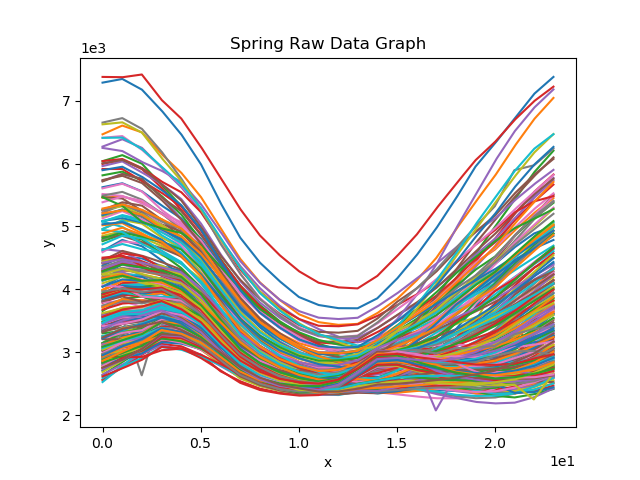
\includegraphics[height=1.8in]{Spring_Raw_Data_Graph_line.png}
        \caption{\small \sl Raw \ac{aps} Spring Demand Data. x is in hours (the 24 hours in a day). y is APS's electric demand in MWe.}
    \end{subfigure}
     \hfill
    \begin{subfigure}[t]{\textwidth}
        \centering
        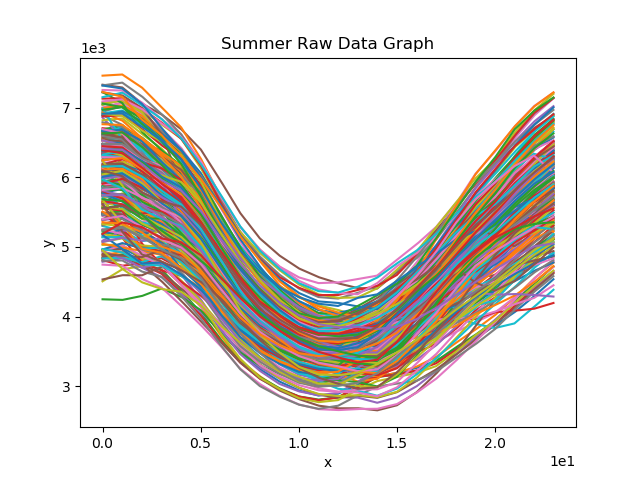
\includegraphics[height=1.8in]{Summer_Raw_Data_Graph_line.png}
        \caption{\small \sl Raw \ac{aps} Summer Demand Data. x is in hours. y is APS's electric demand in MWe.}
    \end{subfigure}
    \vskip\baselineskip
    \begin{subfigure}[t]{\textwidth}
        \centering
        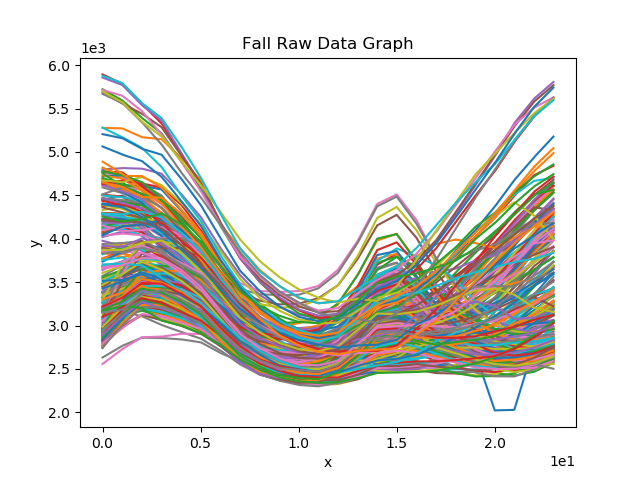
\includegraphics[height=1.8in]{Fall_Raw_Data_Graph_line.png}
        \caption{\small \sl Raw \ac{aps} Fall Demand Data. x is in hours. y is APS's electric demand in MWe.}
    \end{subfigure}
    \quad
    \begin{subfigure}[t]{0.9\textwidth}
        \centering
        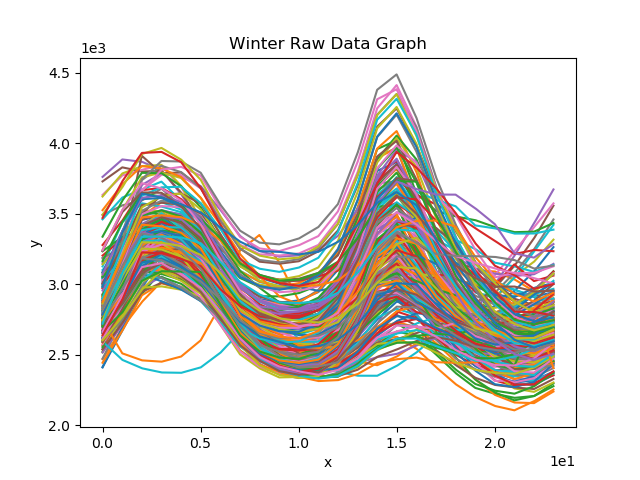
\includegraphics[height=1.8in]{Winter_Raw_Data_Graph_line.png}
        \caption{\small \sl Raw \ac{aps} Winter Demand Data. x is in hours. y is APS's electric demand in MWe.}
    \end{subfigure}

    \caption{\small \sl Raw data showing general Arizona Public Service Demand from the EIA from July 1st, 2015 to May 18, 2018}
    \label{RawDemand}
\end{figure*}

\begin{figure*}[t!]
    \centering

    \begin{subfigure}[b]{0.9\textwidth}
        \centering
        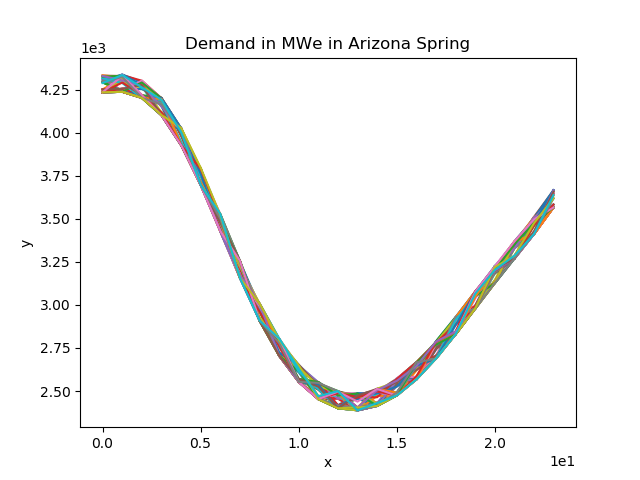
\includegraphics[height=1.8in]{Demand_in_MWe_in_Arizona_Spring_line.png}
        \caption{\small \sl Spring \ac{aps} Demand Data. x is in hours (the 24 hours in a day). y is APS's electric demand in MWe.}
    \end{subfigure}
     \hfill
    \begin{subfigure}[t]{0.9\textwidth}
        \centering
        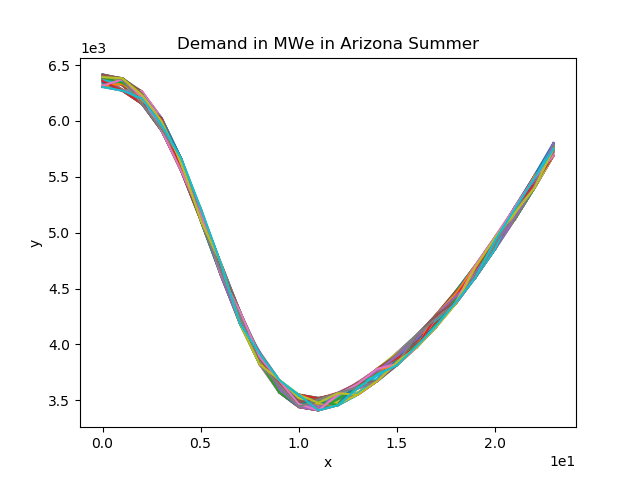
\includegraphics[height=1.8in]{Demand_in_MWe_in_Arizona_Summer_line.png}
        \caption{Synthetic \ac{aps} Summer Demand Data. x is in hours. y is APS's electric demand in MWe.}
    \end{subfigure}
    \vskip\baselineskip
    \begin{subfigure}[t]{0.9\textwidth}
        \centering
        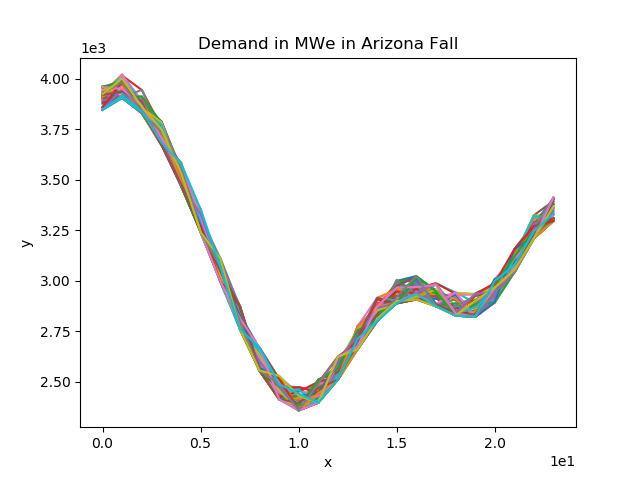
\includegraphics[height=1.8in]{Demand_in_MWe_in_Arizona_Fall_line.png}
        \caption{\small \sl Synthetic \ac{aps} Fall Demand Data. x is in hours. y is APS's electric demand in MWe.}
    \end{subfigure}
    \quad
    \begin{subfigure}[t]{0.9\textwidth}
        \centering
        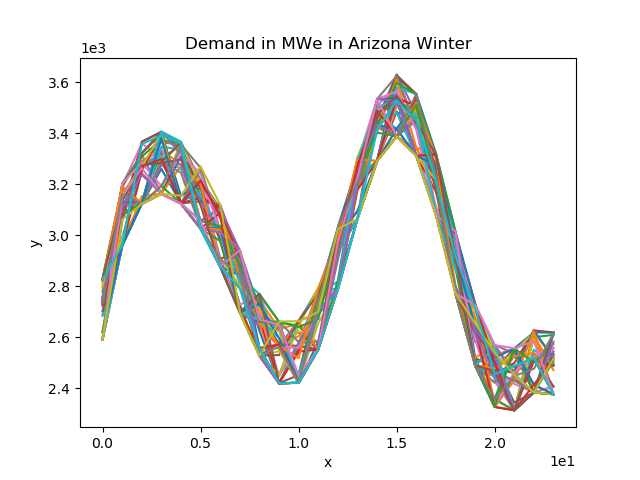
\includegraphics[height=1.8in]{Demand_in_MWe_in_Arizona_Winter_line.png}
        \caption{\small \sl Synthetic \ac{aps} Winter Demand Data. x is in hours. y is APS's electric demand in MWe.}
    \end{subfigure}
    \caption{\small \sl Cleaned up Synthetic Data showing general Arizona Public Service Demand}
    \label{SyntheticAverage}
\end{figure*}

\clearpage

\begin{table}[h!]
\centering
\caption{Approximate average values for demand change in Arizona for each season}

\begin{tabular}{|l|l|l|l|l|l|}
\hline
\multicolumn{1}{|c|}{\textbf{Season}} & \multicolumn{1}{c|}{\textbf{\begin{tabular}[c]{@{}l@{}}Peak\\ Demand\\ (MWe)\end{tabular}}} & \textbf{\begin{tabular}[c]{@{}l@{}}Minimum\\ Demand\\ (MWe)\end{tabular}} & \textbf{\begin{tabular}[c]{@{}l@{}}Change in\\ Demand\\ (MWe)\end{tabular}} & \textbf{\begin{tabular}[c]{@{}l@{}}Local\\ Minimums\\ (MWe)\end{tabular}} & \textbf{\begin{tabular}[c]{@{}l@{}}Change in \\ Local\\Demand (MWe)\end{tabular}} \\ \hline
Spring                                & 4300                                      & 2320                                                              & 1980                                                                & N/A                                                               & N/A                                                                        \\ \hline
Summer                                & 6400                                      & 3500                                                              & 2900                                                                & N/A                                                               & N/A                                                                        \\ \hline
Fall                                  & 3900                                      & 2350                                                              & 1550                                                                & 2950                                                              & 950                                                                        \\ \hline
Winter                                & 3500                                      & 2450                                                              & 1050                                                                & 2500                                                              & 1000                                                                       \\ \hline
\end{tabular}
\label{DemandChange}
\end{table}


\subsection{Fluctuation Analysis}

As determined by the RAVEN assessment shown in table \ref{DemandChange}, the flexible operation of Palo Verde currently required due to demand variability are greater than the amount of power APS owns from Palo Verde for all months besides winter.  If APS chooses to use Palo Verde as a major tool for load following, it would be most helpful to shift most of the load to uses other than the grid for portions of the day.  Clearly, as shown in table \ref{DemandChange} and figure \ref{SyntheticAverage}, the transition from maximum electric demand to minimum electric demand is not a sharp drop off at one point in the day, but more of a gradual transition.

As figures \ref{SyntheticAverage}, \ref{RawDemand}, and table \ref{DemandChange} demonstrate, the load change over a day would generally require that all of the electricity be diverted from the APS-owned load from Palo Verde if following strictly with the nuclear generation.  Since the demand curves typically decrease and increase over several hours, the load would have to be shifted to water production in portions over the day if load following just with Palo Verde.  The various exergy and revenue outcomes from the thermally and electrical coupled systems at different rates of load following have already been detailed in tables \ref{LoadFollow}, \ref{SW-S} and \ref{SW-L}. The tendency for the demand to shift gradually would suggest a benefit to electrically coupling, which does not have thermal hydraulic feedbacks from shifting. Overall, if load following just with the load APS owns from Palo Verde, there would not be sufficient change, even if decreasing the load to zero to load follow in any season besides from winter.

APS owns and operates natural gas and coal power plants which are the more traditional generation sources that vary output. Looking at figure \ref{SyntheticAverage}(d) reflecting the total winter demand hovering below 2000 MWe on some days, it is very plausible that sometimes renewable generation will make up over 900 MWe during that period and APS will have too much generation even with all the coal and natural gas removed from the grid.

\section{Conclusions}
\begin{itemize}
\item The MSF unit combined with the condenser has the greatest overall \$/exergy value at 10\% of the load sent to water production.
\item The reverse osmosis systems all had greater values for \$/exergy besides the 10\% load follow of the MSF coupled to the condenser.
\item Palo Verde Generating Station will need to flexibly operate to deal with the increasing level of variable penetration in both Arizona and California.
\item Generating sufficient water to meet 20\% of Palo Verde's water needs does not require a lot of load following.
\item The water purification systems that are reasonably sized would not require as much power as Palo Verde needs in order to make up for the overproduction on the grid at times.
\item Comparing thermally and electrically coupled systems requires finding a process that purely uses heat and comparing that process with heat from the reactor and heat converted from electricity in the reactor.  The analysis done here ends up comparing two separate industrial processes and thus does not evaluate the benefits of a thermally versus an electrically coupled system.
\end{itemize}



\chapter{Future Work and Conclusions}
\label{Chapter:FWAndConclusions}
% Add an analysis section

The work performed in this thesis seeks to add to the growing body of knowledge surrounding Nuclear Renewable Hybrid Energy Systems as a solution for nuclear power plants and renewable energy sources to work in tandem to decarbonize both the electric and industrial sectors in an economically profitable way. There is much more work to be done both on this particular example of coupling a water purification system to a Palo Verde plant as well as more generally in determining the appropriate application of NRHESs. Some of the future work suggested includes:

\begin{itemize}
\item Include flexibility in a more dynamic manner instead of a qualitative assessment of the differences between MSF and RO desalination.
\item Quantify the quality of the product produced with the two different approaches.  The RO system would produce high quality water initially while a MSF system would require some startup time, a feature which was not quantified in this analysis.
\item Include a financial value for flexibility and the resilience provided to a nuclear power plant that produces its own water.
\item Further develop the Specific Exergy Revenue thermoeconomic approach to include multiple products.
\item Perform a sensitivity analysis of the exergy economics analysis to the price of water and electricity.
\item Compare the nuclear exergy analysis with a coal plant and concentrated solar analysis to see how the thermodynamic properties of various heat sources compare.
\item Model a battery system, such as compressed air, instead of the water purification system to compare the thermodynamic and economic benefits of both.
\item Perform an economic assessment of the revenue lost if nuclear plants were asked to curtail, then slowly ramp back up, as opposed to sending electricity to an industrial process.
\item Conduct an analysis of a combination of thermal heat and electric power using some of the waste heat from the reactor to pre-heat the water entering the reverse osmosis system.
\item Use more realistic pumps for the RO system.  The three pumps included in this analysis are off-the-shelf options for RO systems.  The RO system would likely be tailored to the use case for Palo Verde.
\item Use a more precise power cycle and thoroughly determine the thermalhydraulic feedbacks included with thermal coupling.
\item Include capitol and maintenance costs for the water purification systems.
\item Focus on taking individual turbines off of the system as opposed to specific loads.  Taking each of the four turbines off of the system and sending that heat to a water purification system may be a better management technique for the power plant.
\item Include a more thorough analysis of how bypassing heat exchangers or using reheaters in the power cycle would affect the overall exergetic efficiency.
\item Include a regulatory review and investigation to analyze the likely regulatory complexities of thermal versus electrical coupling of industrial processes.
\end{itemize}

Some of the future work to be done on applying AHP to decision making in NRHES include ensuring that the characteristics included in the analysis are valuable relative measures as opposed to strictly meeting a standard. The safety and ability to fluctuate characteristics should meet a certain clearly defined standard.  A comparative approach was inappropriate for characteristics that either meet a standard or do not.

\section{Summary Remarks}
 There were multiple approaches taken in this thesis to analyze how to progress in the modeling and development of NRHESs. The initial literature review discussed the progression of typically smaller traditional \ac{hes}s as well as the development up to this point for \ac{nrhes}s.  The literature review concluded that future research on modeling NRHESs should compliment the ongoing work modeling NRHESs using the Modelica language and RAVEN.  While the ongoing modeling focuses on questions surrounding how to optimize a NRHES based on minimizing cost, Chapter \ref{TvsE} focused on comparing the thermodynamic and economic benefits of electric and thermal coupling of two different water purification systems. Chapter \ref{Risk} focused on applying two risk assessment techniques, \ac{pha} and \ac{ahp}, to a NRHES.  The chapter discussed the benefits of applying risk assessment techniques early to large capital intensive projects to minimize financial and safety risks.  The chapter also discussed an applied expert AHP survey.  While the fuzzy logic applied to the survey suggested that desalination was the best industrial process to include in a NRHES, that conclusion primarily came from the large emphasis placed on safety.  Future AHP applications should focus on characteristics of the system which do not need to meet clearly defined standards.  The safety and ability to fluctuate characteristics used the in the AHP have clearly defined legal standards which are either met or not met.  Chapter \ref{TvsE} focused on comparing the thermodynamic and economic benefits of coupling a water purification system to Palo Verde Generating Station. It found that in general a multi stage flash distillation system thermally coupled to a nuclear power plant has better exergetic economics, but is worse overall both for revenue as well as due to the added complexity for building and moving heat with a thermally coupled system.

 In conclusion, Nuclear Renewable Hybrid Energy systems propose a possible solution allowing nuclear power plants to fluctuate along with grid demand and renewable generation.  When the price of electricity is very low, there is an economic benefit to selling the heat or electricity to a water distillation system for the Palo Verde Nuclear Power Plant. Also, as the price of water continues to increase in value, there is an economic benefit to producing more water. At current average prices for electricity, there is no revenue advantage to generating water as well as electricity.  The benefits from the ability to fluctuate as well as the stability of generating sufficient water for the power plant have not been included in the economic assessment. These characteristics do have a value which needs to be included in future assessments. While there is a lot of work to be done analyzing hybrid energy systems, there is some promise that, depending on the price for electricity and water, they could have a valuable role in meeting human resource needs.


% The refs.bib file contains examples of how to put these three sources into the .bib. See REFERENCES
  % below for more notes and ideas for this section.  % Period should follow citations at end of sentence

% Go to a new page, and flush all pending flats from stack. Start the chapter "fresh"
\clearpage

% ========================================= REFERENCES =========================================== %
% Put your references in a separate .bib file. You can manually enter the information in that file,
  % but it's easiest to use a tool like Mendeley or Zotero to manage your sources. They allow you to
  % copy individual sources or groups of sources as .bibtex entries that can be pasted into the .bib.
  % You can also export whole libraries or projects in those programs as a single .bib file.
% It's not a bad idea to briefly annotate your sources in the .bib file (comment above entry) to
  % help locate sources without spending a lot of time looking it up again, especially because you
  % will likely be writing this thing for a year or more.

% Relabel bibliography title as "References"
\renewcommand\bibname{References}
% Add to table of contents, as bibliography usually is not in ToC
\addcontentsline{toc}{chapter}{\textsc{\bibname}}
% Set style. "plain" is fine, or you can look up other ones to play with
\bibliographystyle{ieeetr}
% Name of separate bibliography file containing your references. Using separate file allows the same
  % .bib file on papers and so forth. Also, most reference managers (Mendeley, Zotero, etc) will
  % export .bib files, making this whole process much easier.
\bibliography{example-bib-file.bib}

\newpage

% ========================================= APPENDICES =========================================== %
% Marks start of appendices. Each appendix is marked as a chapter, and each \chapter will be
  % rendered as a separate appendix and appear separately in the ToC.

% ==------------------------------------- Appendix A: ... --------------------------------------== %
% --------------------------------------------------------------------------
% -- Appendices --
\clearpage
\appendix  % Marks start of appendices
\chapter{Expert AHP Survey}

The description for the survey which includes all of the assumptions built into the survey is:

The following questionnaire will take 10 to 20 minutes to complete. Thank you for your time and consideration.

The questionnaire below is one part of my research evaluating the potential benefits of applying the risk assessment technique of Analytic Hierarchy Process (AHP) to compare different industrial processes that might be incorporated into a nuclear renewable hybrid energy system.  AHP requires a group of experts determining the relative values associated with each of the options being compared.  The questionnaire  requests your expert opinion on determining the values associated with thermally coupling a desalination plant, a synthetic fuels plant, and a hydrogen production plant to a nuclear power plant.  The three industrial processes are compared based on safety, flexibility, and economic value.

This survey assumes that the process used for hydrogen production is high temperature steam electrolysis with thermal as well as electrical coupling to the nuclear power plant.  The assumed form of desalination is thermal desalination through distillation directly using heat from the nuclear power plant.  The assumed synthetic fuel process is a Fischer-Tropsch method using coal as the hydrocarbon source.  Assume each of the processes consumes the same amount of heat from the nuclear power plant.

The questions below deal with the relative value of each of the industrial processes based on each of the characteristics taken into consideration in this study: safety, ability to fluctuate, and profitability. Ability to fluctuate describes how difficult it is to start and stop the industrial process, as well as the ability of the industrial process to ramp to allow more or less heat to be allocated to electricity production to match demand from the grid. For example, if the process can start and stop, but the initial batch of product is of lower quality, that would negatively affect the "ability to fluctuate" as compared to a process that could start and stop with no impact on the initial batch of product after restarting.  An industrial process that could more or less instantaneously reach full capacity steady state operation would rank higher than an industrial process that would take a long time to reach full capacity steady state operation.

For AHP,  the range of the scale is from 1 to 9, with 1 representing when the two options are thought of as equal for the given characteristic. As can be seen below with the safety comparison of desalination to hydrogen production, you will have three initial options. If you choose that the desalination and hydrogen production are equally safe, that will be recorded as a 1 in the AHP. If you choose, for example, that hydrogen production is safer than desalination, then you will be directed to a second question which determines your view of how much safer hydrogen production is than desalination.

As AHP focuses on collecting expert opinions, you have been selected because you have either published research or a report on nuclear renewable hybrid energy systems, cogeneration, or have worked with a nuclear cogeneration system. I would appreciate it if I could include your name as participating in the research, as can be seen in the first question below.  Your answers will not be shared, only that you were part of the expert group taking this survey.

I recognize that characteristics such as regional accessibility of feedstocks for each of the industrial processes will have a major impact on which industrial process would be pursued in a nuclear renewable hybrid energy system. For the purposes of this research, please assume all regional characteristics are equal.  The goal of this research is to ascertain whether AHP can generally be applied to determining the relative values of different potential industrial processes for a nuclear renewable hybrid energy system.

Thank you for your time and willingness to participate in this research. If you have any questions about the survey, please contact me at:

Emma Redfoot
redf3263@vandals.uidaho.edu
(406) 876-2026
Graduate Research Assistant
University of Idaho
% Appendices are done as LaTeX chapters
% \chapter{Expert AHP Survey}
% \label{ExpertAHP}


\includepdf[pages={2-}]{AHP_survey.pdf}

\chapter{Fuzzy Analytic Hierarchy Process}
\label{App:FAHP}

The following code includes how the fuzzy AHP was performed on the expert AHP survey described above.  The process first involved translating the responses into the ranges descriptive of each of the answers.  Then, the answers from each of the surveys was input into the program.  Then, a geometric mean was found for each of the responses.  Each of the options were then weighted based on the importance of the characteristics, in this case with safety having a much greater weighting than the other two characteristics.
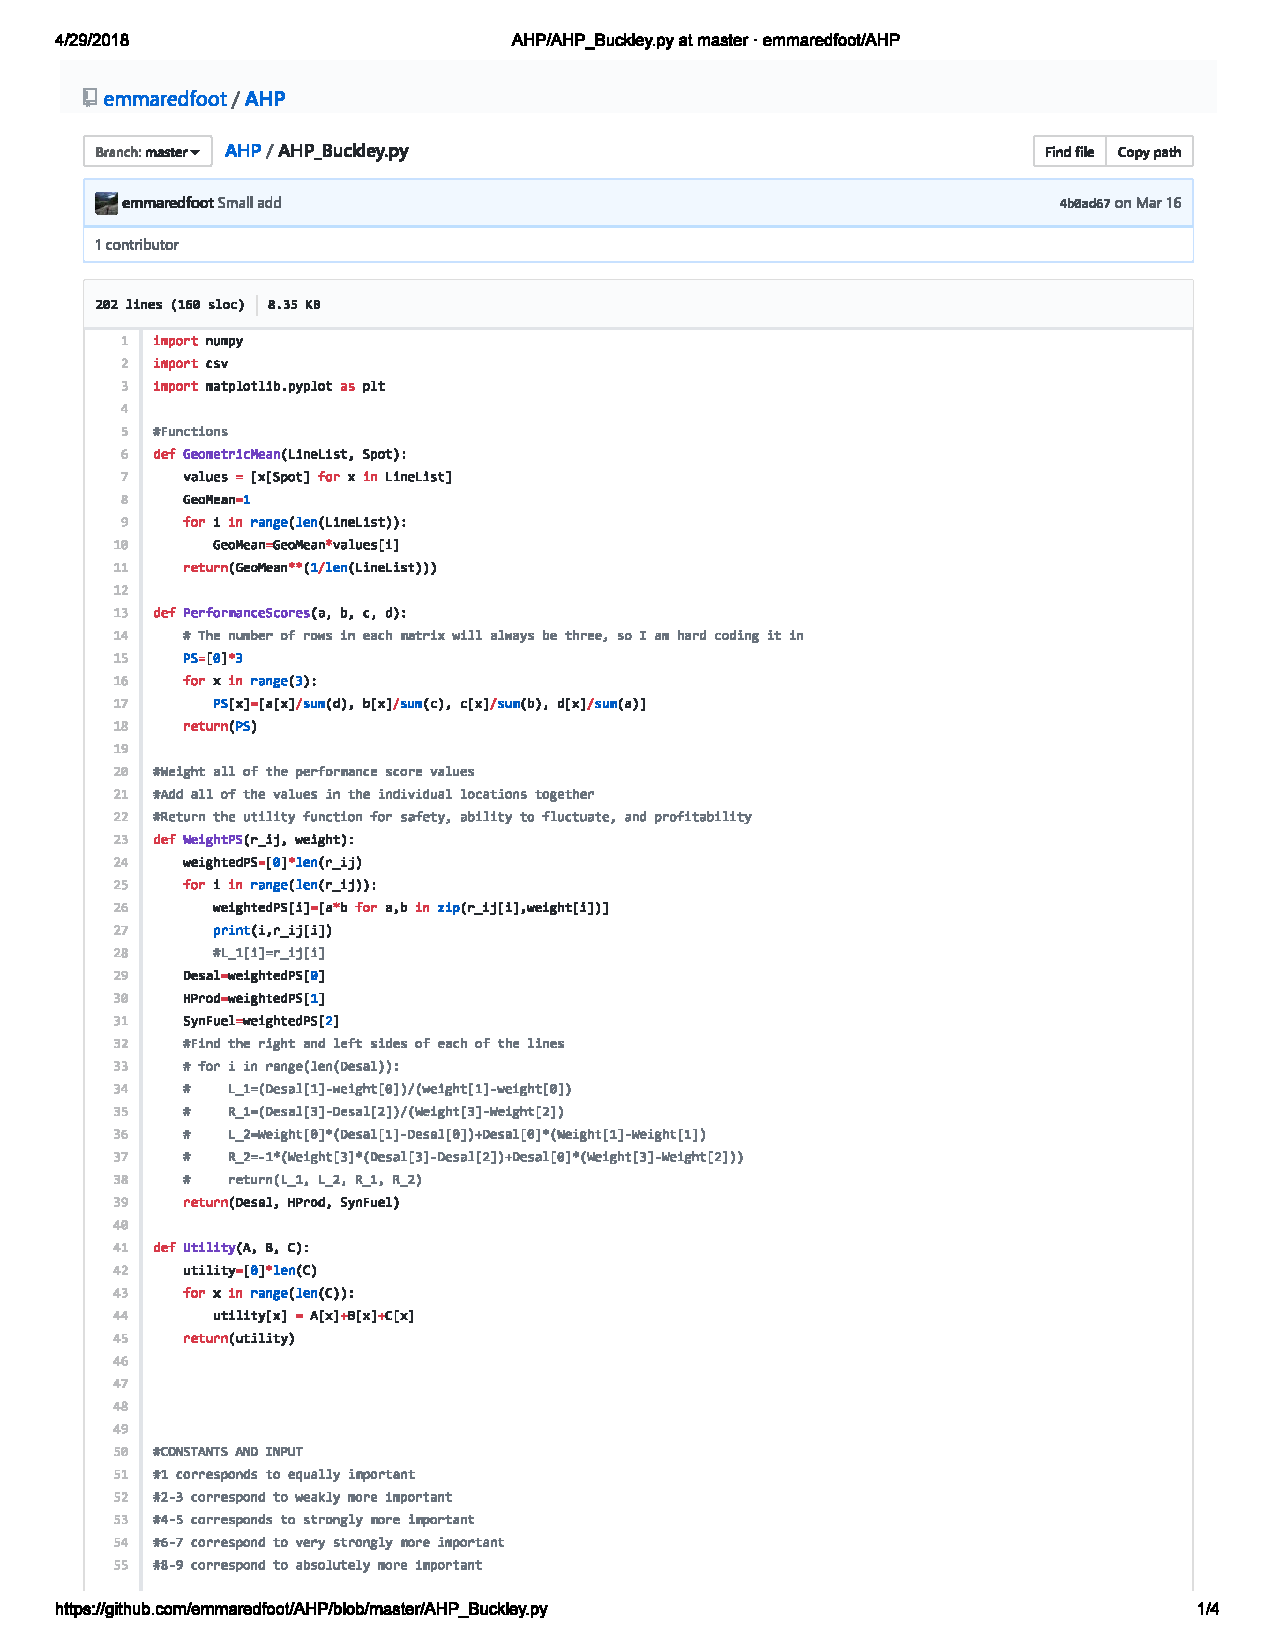
\includepdf{AHP_Buckley_1.pdf}
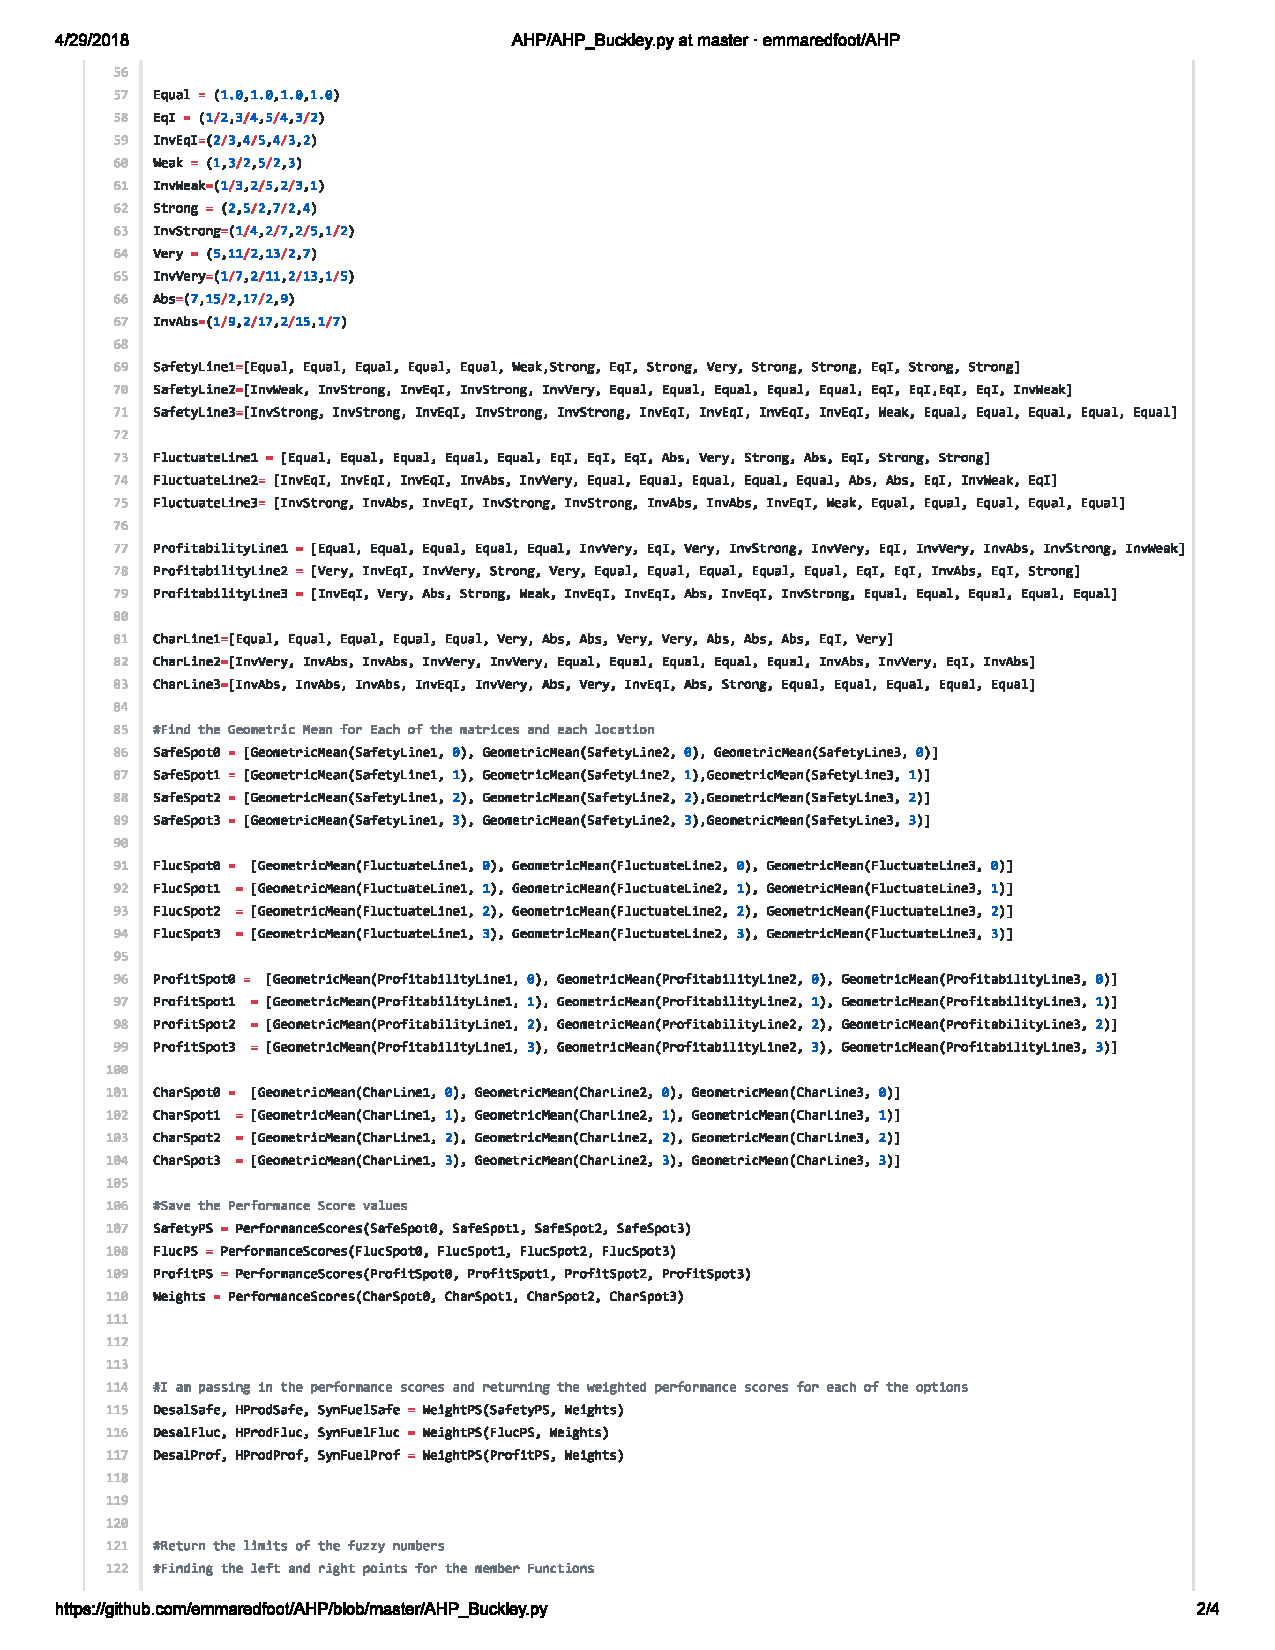
\includepdf{AHP_Buckey_2.pdf}
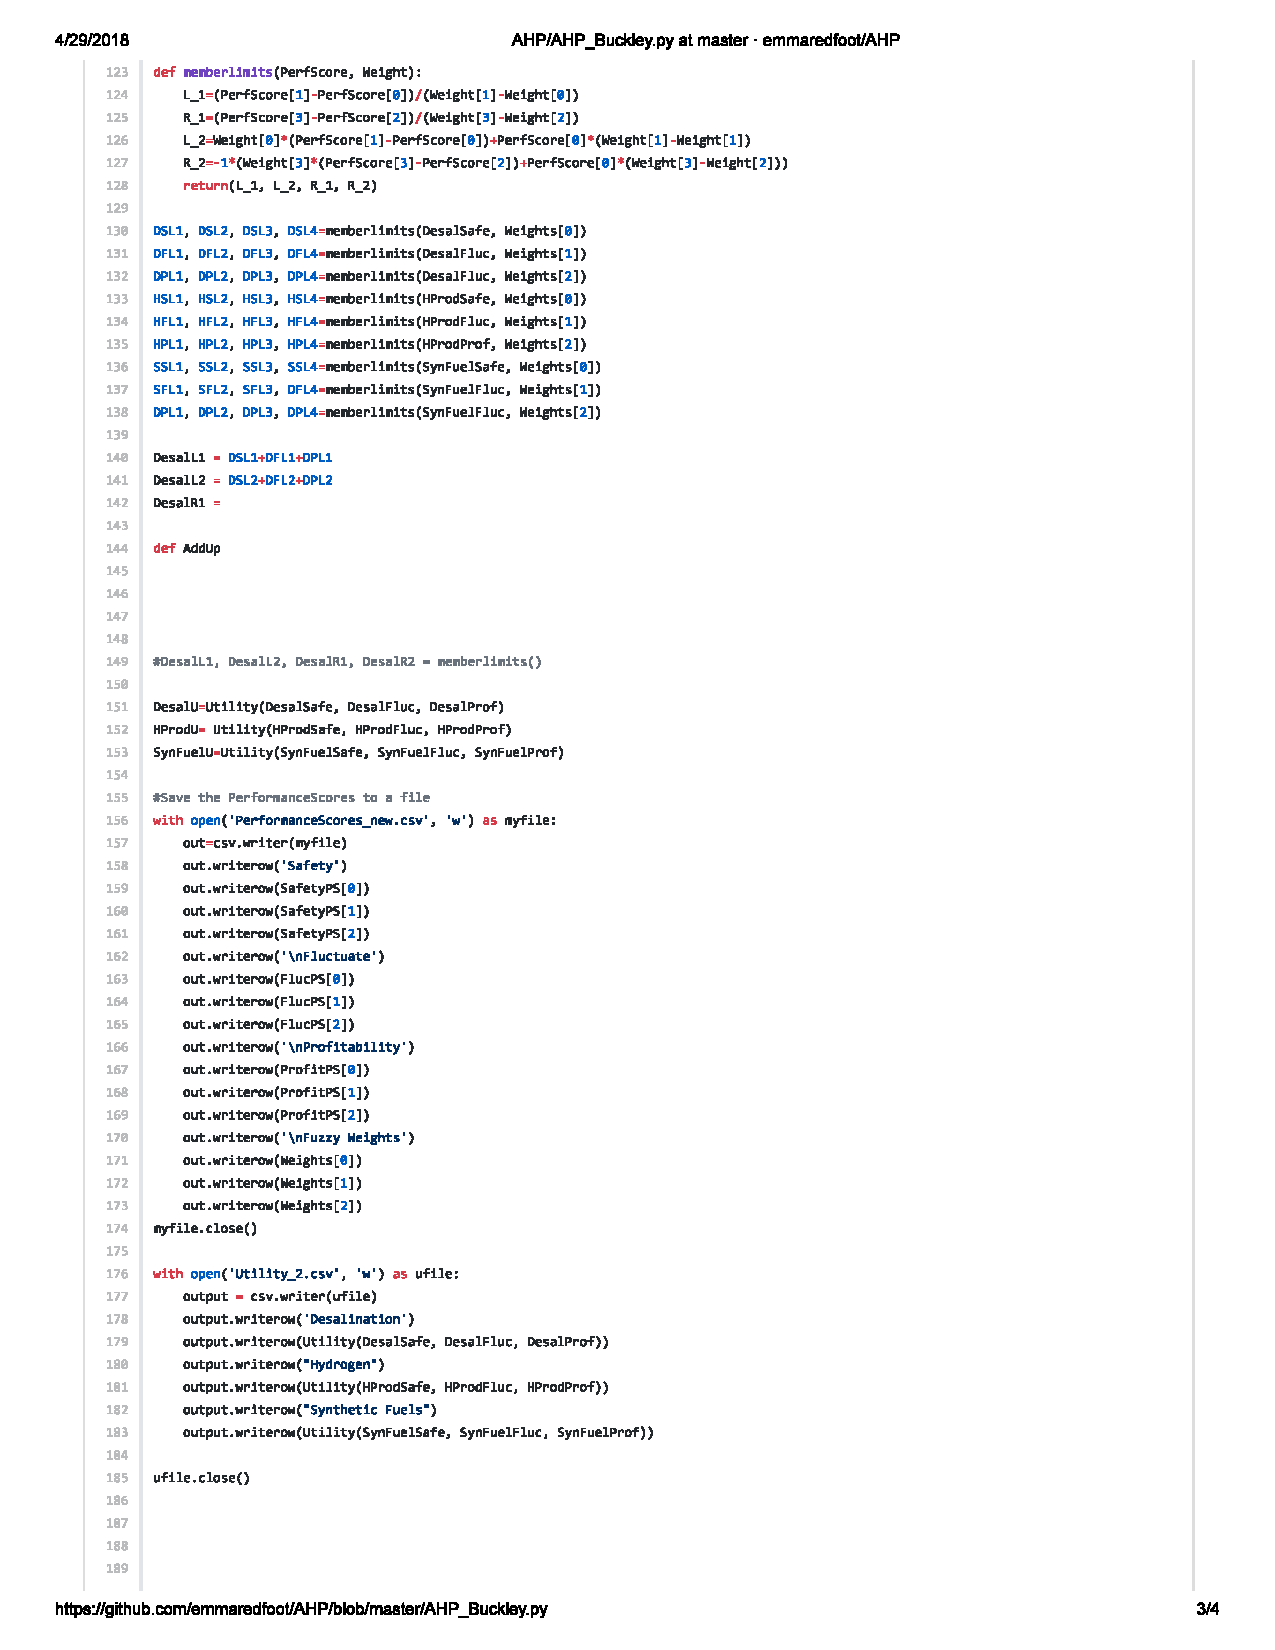
\includepdf{AHP_Buckey_3.pdf}


\chapter{Pump Data}
\label{Appendix:pumps}

The following pump datasheets are the direct sources of information for the off-the-shelf pumps used in this research.  IDE Progreen is the company which constructed the world's largest reverse osmosis system.  These pumps have data including the pressure required for the reverse osmosis system using these pumps. The pressure and energy requirement data from the pump datasheets included are the sources for the pump models developed in Aspen HYSYS.
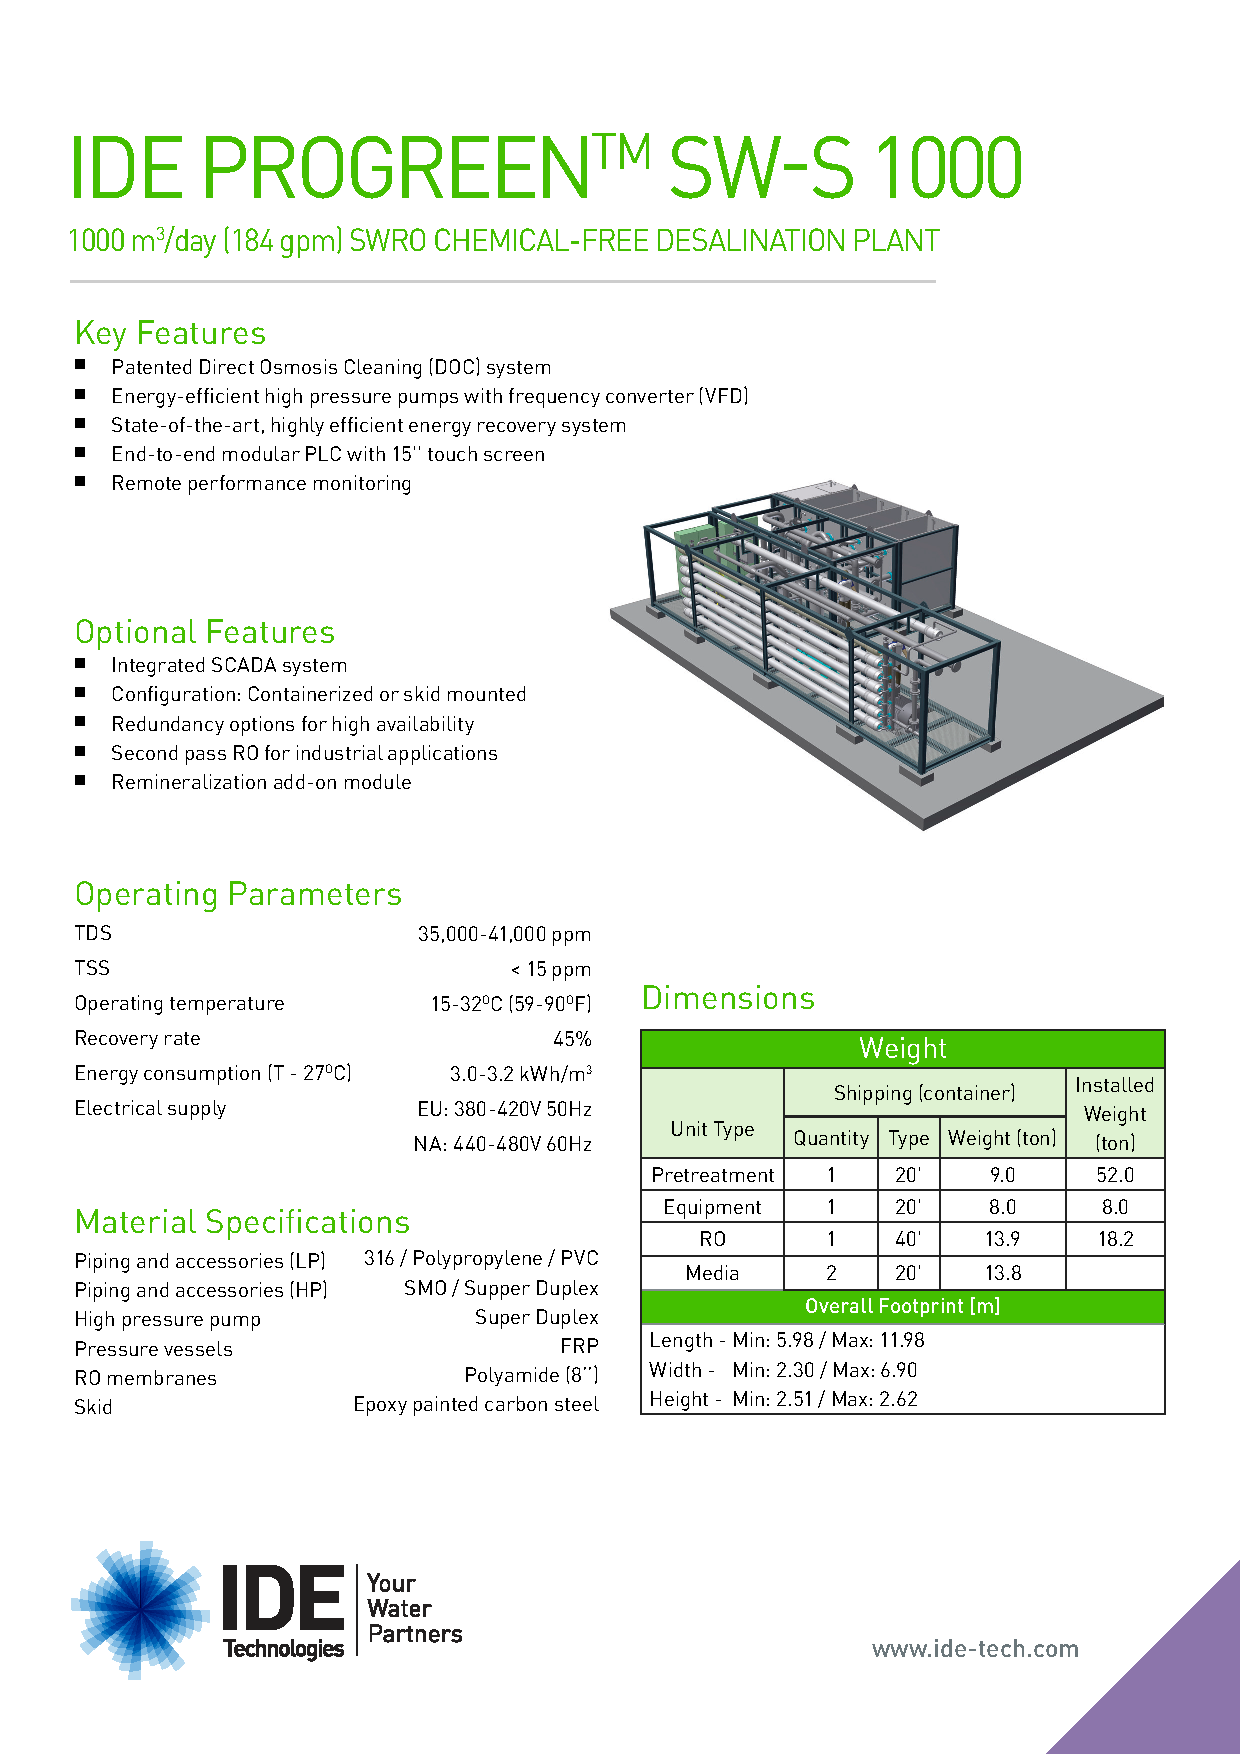
\includepdf[pages={1-}]{IDE-PROGREEN-Datasheet_1000.pdf}
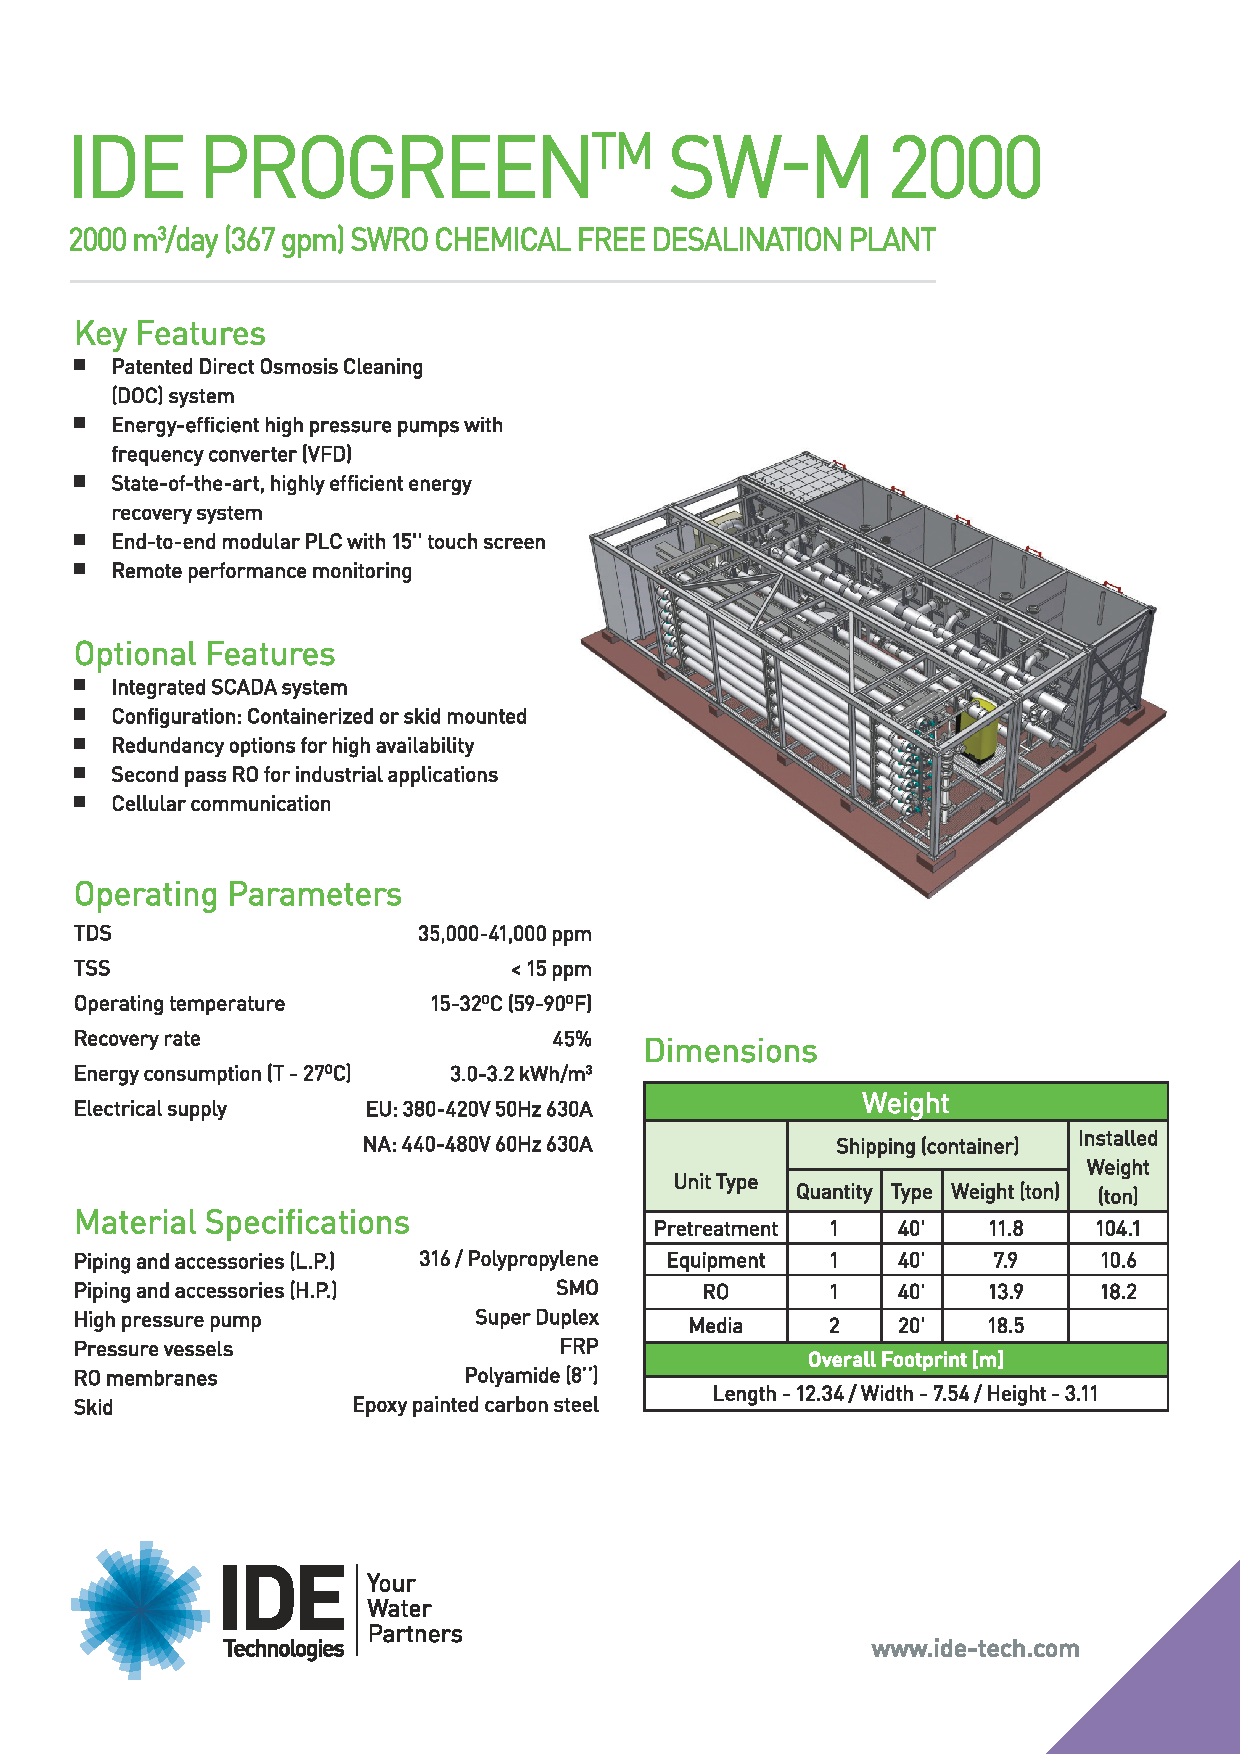
\includepdf[pages={1-}]{IDE-PROGREEN-Datasheet_2000.pdf}
%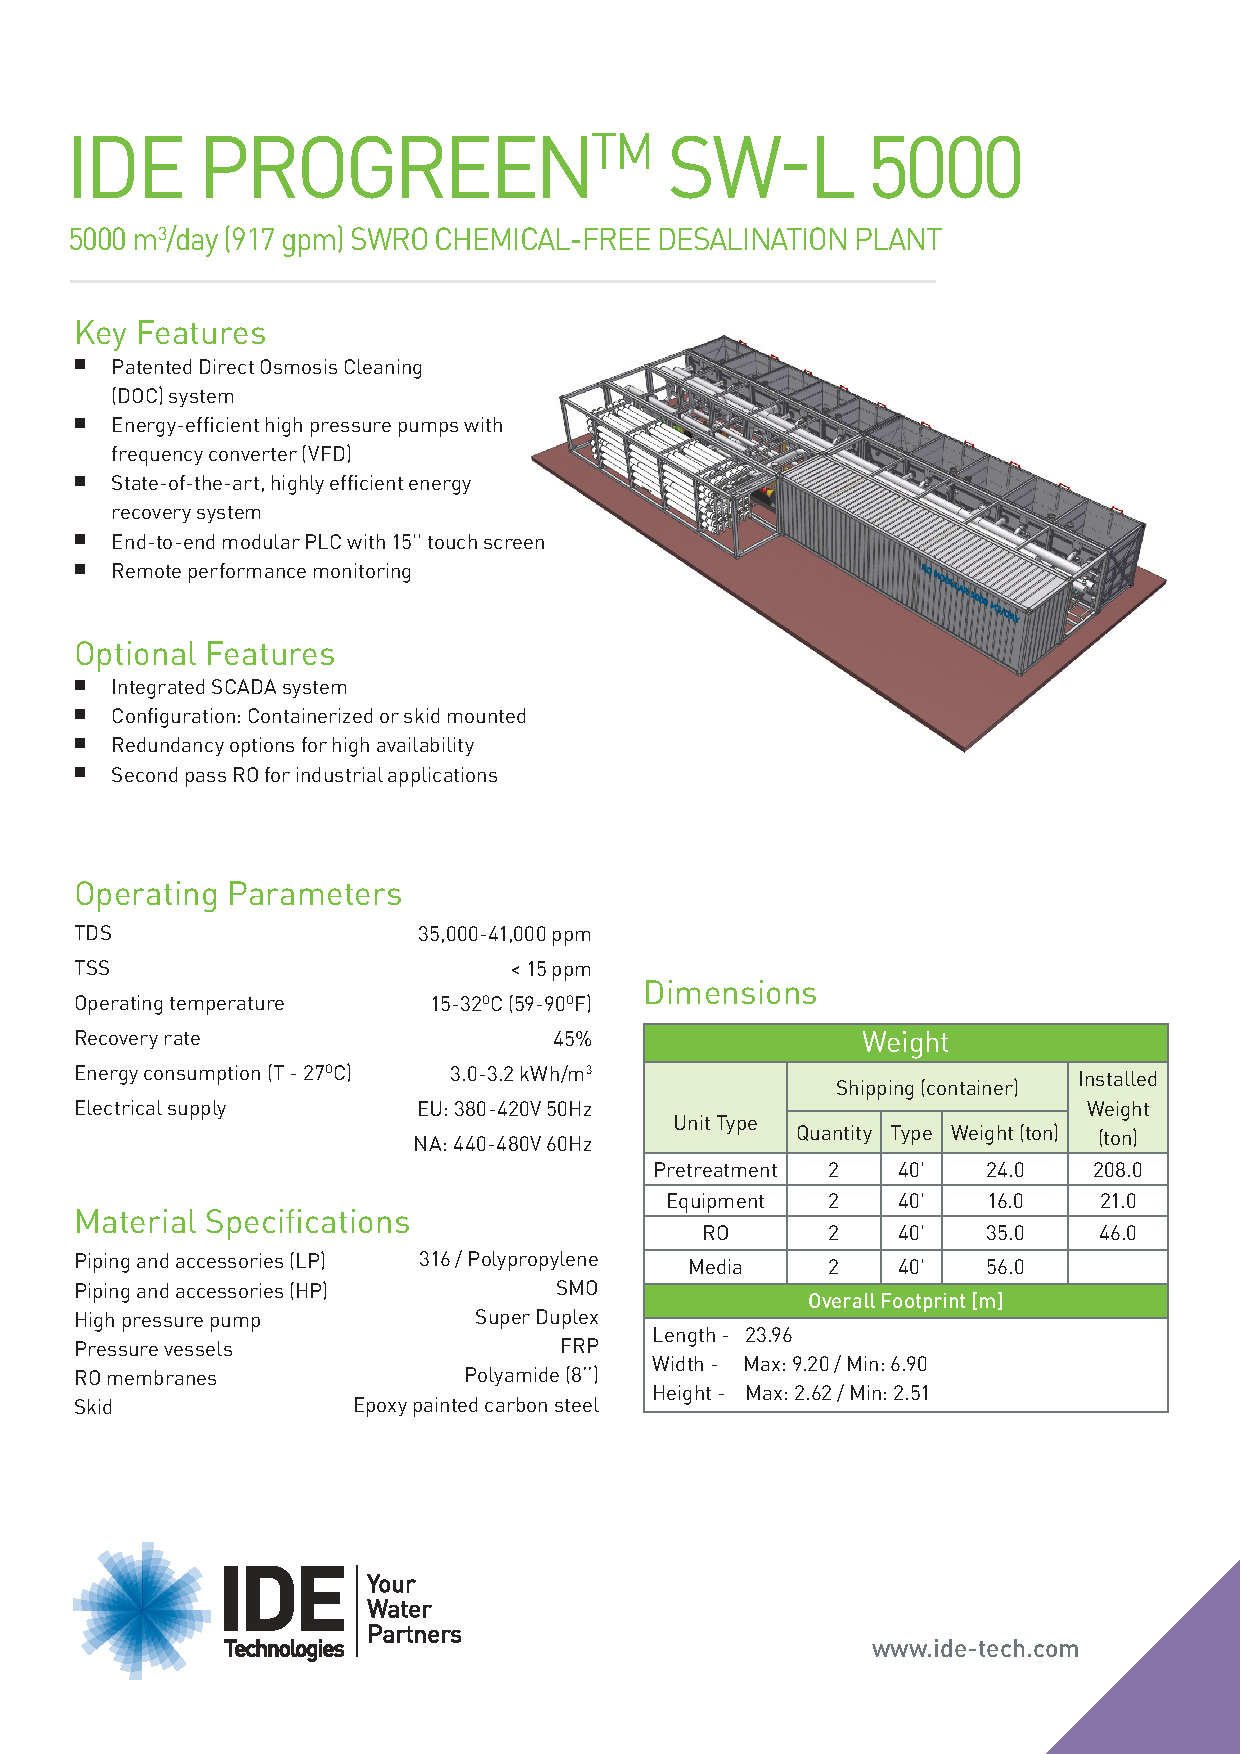
\includepdf[pages={1-}]{IDE-PROGREEN-Datasheet_5000.pdf}

\chapter{Aspen HYSYS}
\label{HYSYSDiagrams}

The following images show some of the MSF and RO configurations included in this thesis.  The MSF system had multiple configurations along with many different temperatures attempted.  Initially, it was unclear if the best configuration would include sending higher temperature water to the MSF system.  After different experiments with the model, it was found that the best outcomes came from running the MSF at 80\degree C.

\begin{figure}
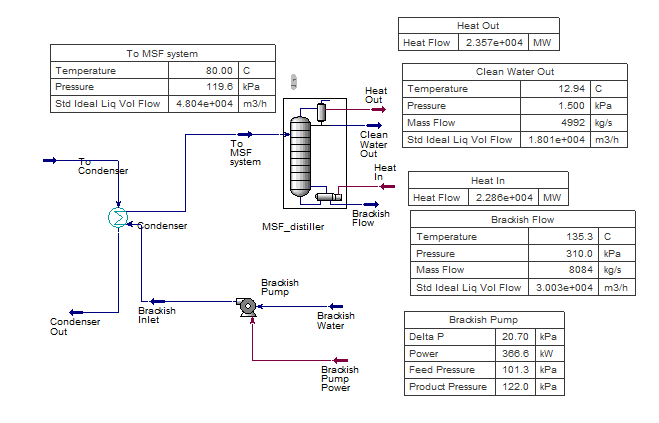
\includegraphics[width=\textwidth]{6_25CondMSF_25.PNG}
\caption{\small \sl A much simplified model of the Palo Verde Generating Station's Power Cycle sending 80\degree C heat to the condenser to be used for the multi-stage flash distillation water purification process. With 25\% of the electricity decreased and sent as heat to the MSF system}
\end{figure}
\begin{figure}
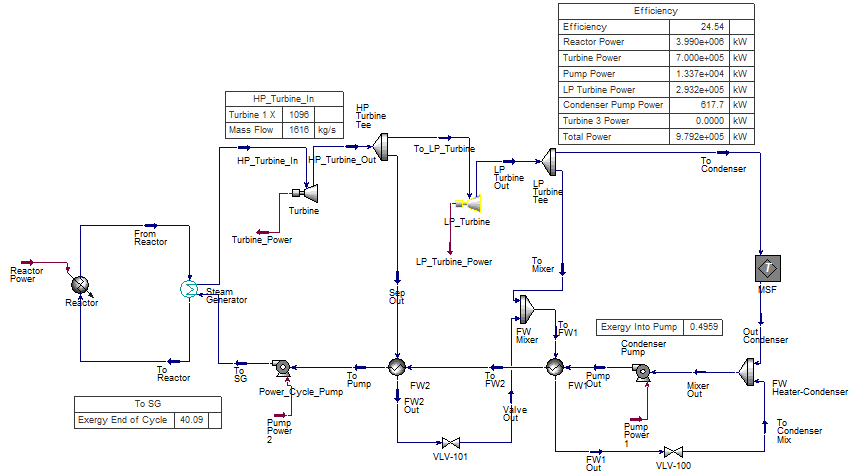
\includegraphics[width=\textwidth]{6_25_CondPC_25.PNG}
\caption{\small \sl A much simplified model of the Palo Verde Generating Station's Power Cycle sending 80\degree C heat to the condenser to be used for the multi-stage flash distillation water purification process. With 25\% of the electricity decreased and sent as heat to the MSF system}
\end{figure}
\begin{figure}
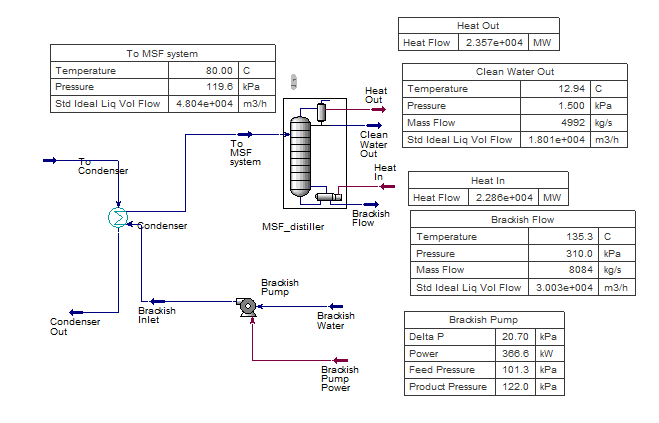
\includegraphics[width=\textwidth]{6_25CondMSF_25.PNG}
\caption{\small \sl A much simplified model of the Palo Verde Generating Station's Power Cycle sending 80\degree C heat to the condenser to be used for the multi-stage flash distillation water purification process. With 25\% of the electricity decreased and sent as heat to the MSF system}
\end{figure}
\begin{figure}
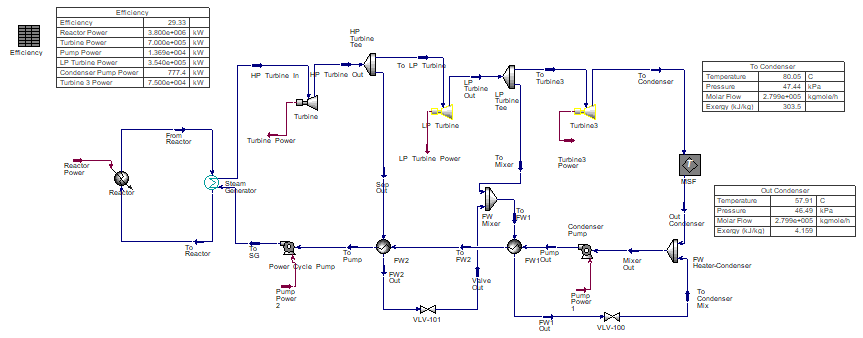
\includegraphics[width=\textwidth]{80PC.PNG}
\caption{\small \sl A much simplified model of the Palo Verde Generating Station's Power Cycle sending 80\degree C heat to the condenser to be used for the multi-stage flash distillation water purification process}
\end{figure}
\begin{figure}
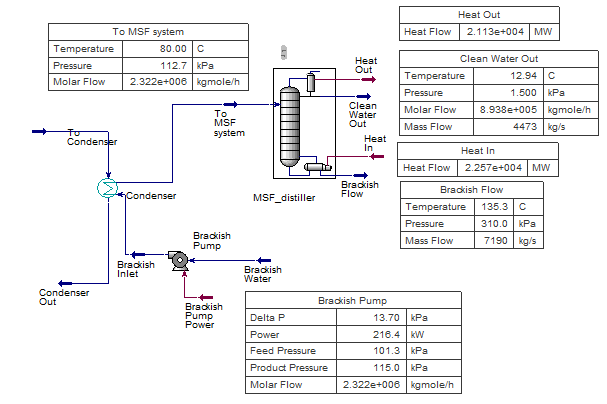
\includegraphics[width=\textwidth]{80MSF.PNG}
\caption{\small \sl A simplified model of a 21 stage multi stage flash distillation system functioning with 80\degree C heat from the reactor to the condenser to be used for the multi-stage flash distillation water purification process}
\end{figure}
\begin{figure}
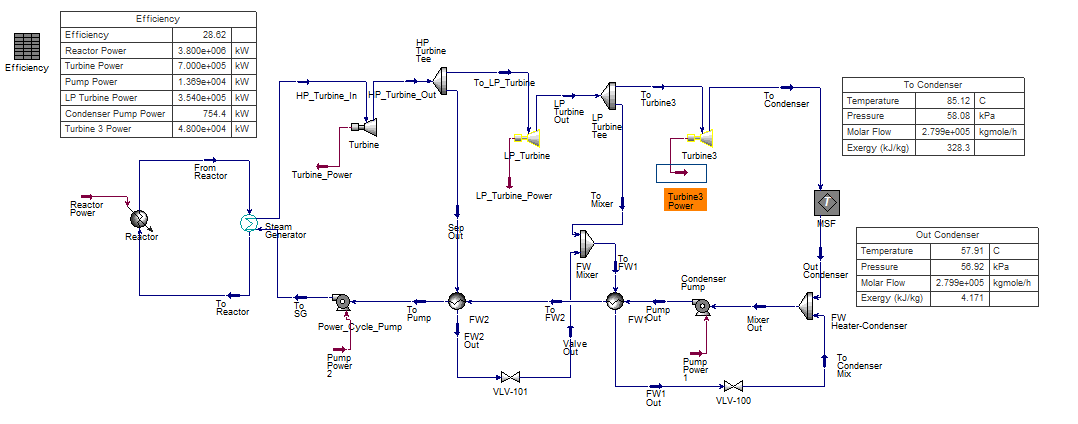
\includegraphics[width=\textwidth]{85PC.PNG}
\caption{\small \sl A much simplified model of the Palo Verde Generating Station's Power Cycle sending 85 \degree C heat to the condenser to be used for the multi-stage flash distillation water purification process}
\end{figure}
\begin{figure}
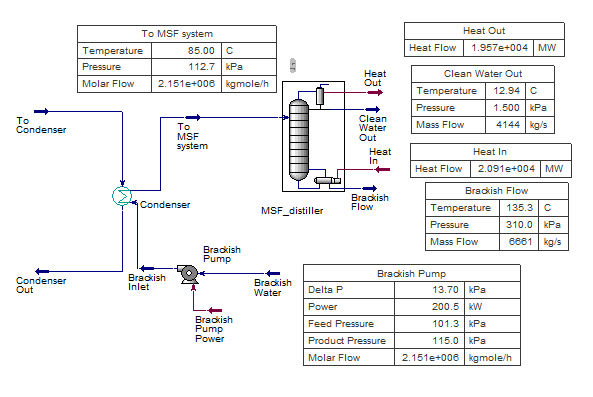
\includegraphics[width=\textwidth]{85MSF.PNG}
\caption{\small \sl A simplified model of a 21 stage multi stage flash distillation system functioning with 85 \degree C heat from the reactor to the condenser to be used for the multi-stage flash distillation water purification process}
\end{figure}
\begin{figure}
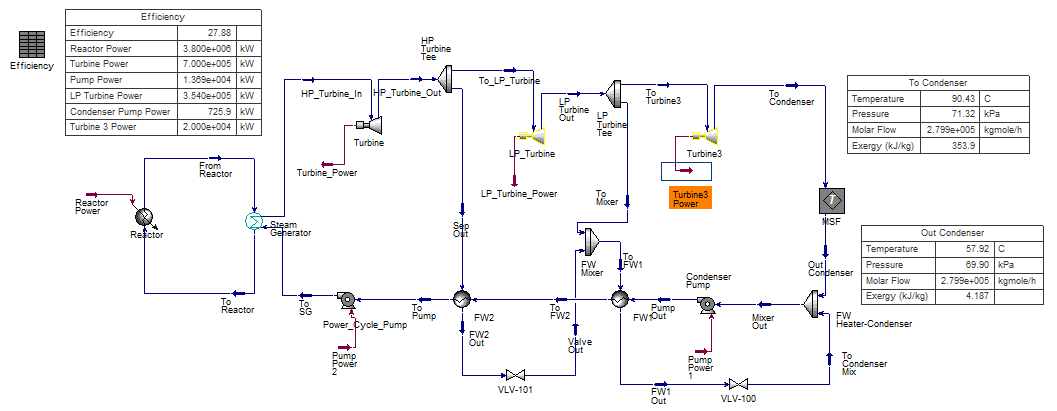
\includegraphics[width=\textwidth]{90PC.PNG}
\caption{\small \sl A much simplified model of the Palo Verde Generating Station's Power Cycle sending 90\degree C heat to the condenser to be used for the multi-stage flash distillation water purification process}
\end{figure}
\begin{figure}
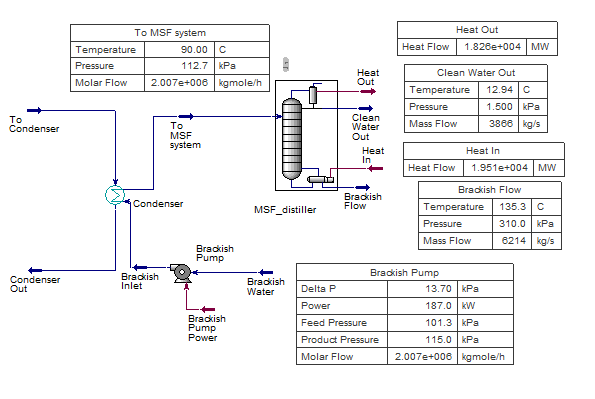
\includegraphics[width=\textwidth]{90MSF.PNG}
\caption{\small \sl A simplified model of a 21 stage multi stage flash distillation system functioning with 90\degree C heat from the reactor to the condenser to be used for the multi-stage flash distillation water purification process}
\end{figure}
\begin{figure}
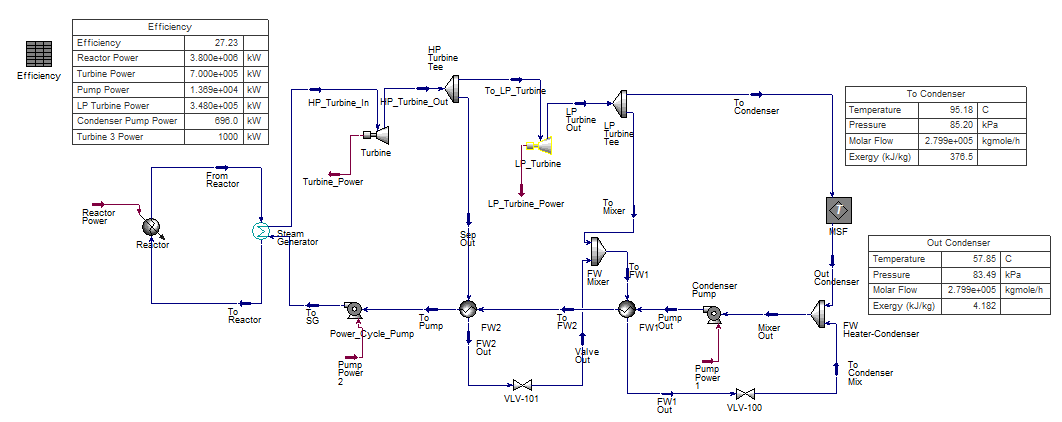
\includegraphics[width=\textwidth]{95PC.PNG}
\caption{\small \sl A much simplified model of the Palo Verde Generating Station's Power Cycle sending 95\degree C heat to the condenser to be used for the multi-stage flash distillation water purification process}
\end{figure}
\begin{figure}
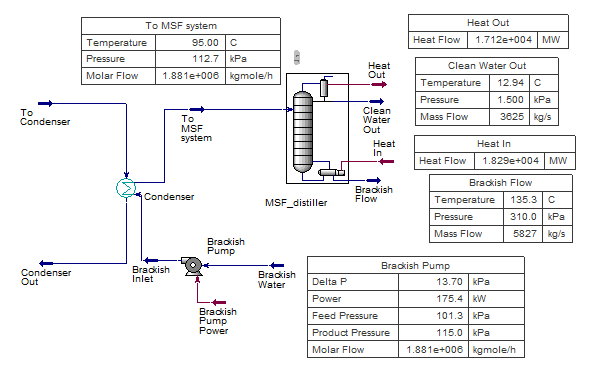
\includegraphics[width=\textwidth]{95MSF.PNG}
\caption{\small \sl A simplified model of a 21 stage multi stage flash distillation system functioning with 95\degree C heat from the reactor to the condenser to be used for the multi-stage flash distillation water purification process}
\end{figure}
\begin{figure}
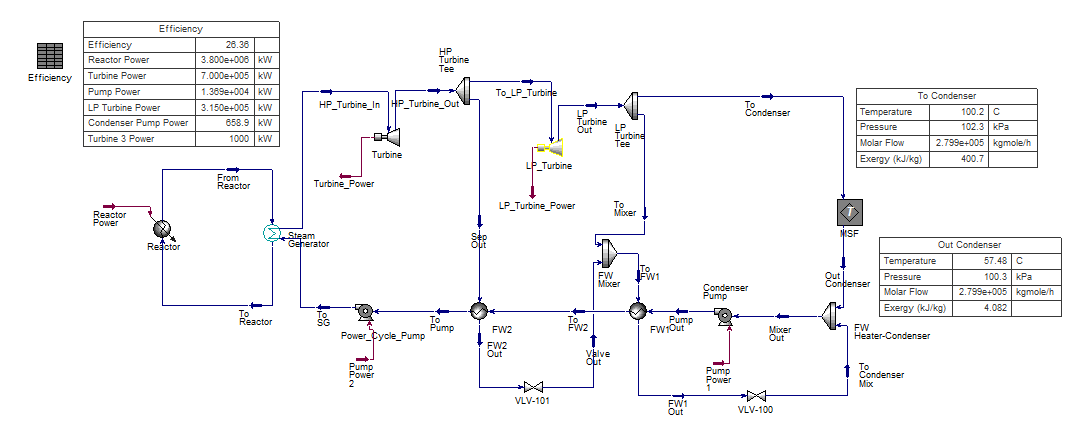
\includegraphics[width=\textwidth]{100PC.PNG}
\caption{\small \sl A much simplified model of the Palo Verde Generating Station's Power Cycle sending 100\degree C heat to the condenser to be used for the multi-stage flash distillation water purification process}
\end{figure}
\begin{figure}
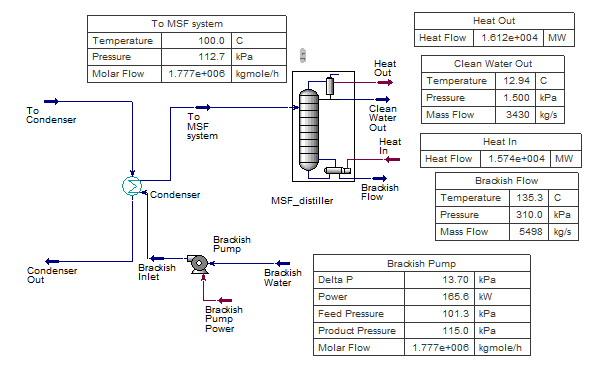
\includegraphics[width=\textwidth]{100MSF.PNG}
\caption{\small \sl A simplified model of a 21 stage multi stage flash distillation system functioning with 100\degree C heat from the reactor to the condenser to be used for the multi-stage flash distillation water purification process}
\end{figure}
\begin{figure*}
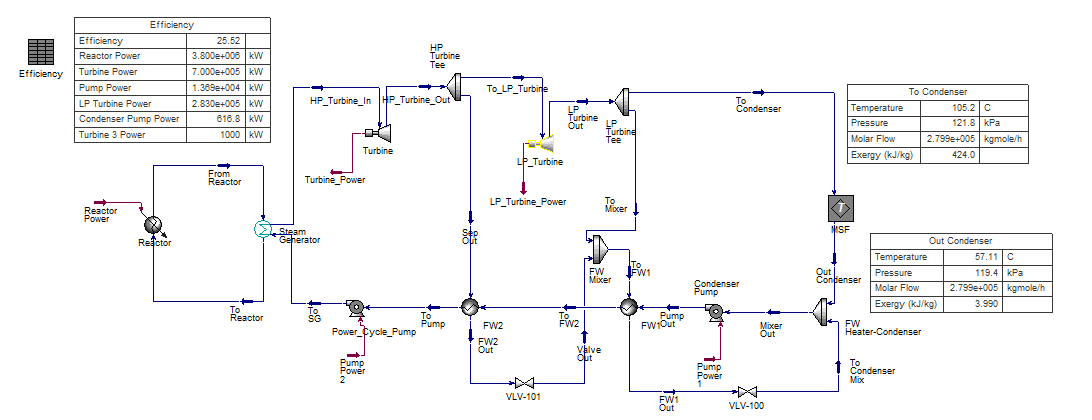
\includegraphics[width=\textwidth]{105PC.PNG}
\caption{\small \sl A much simplified model of the Palo Verde Generating Station's Power Cycle sending 105\degree C heat to the condenser to be used for the multi-stage flash distillation water purification process}
\end{figure*}
\begin{figure*}
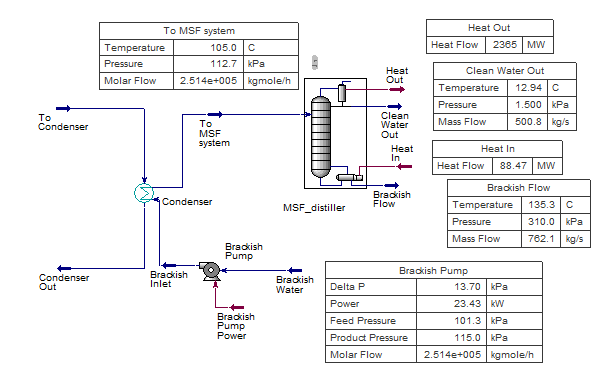
\includegraphics[width=\textwidth]{105MSF.PNG}
\caption{\small \sl A simplified model of a 21 stage multi stage flash distillation system functioning with 105\degree C heat from the reactor to the condenser to be used for the multi-stage flash distillation water purification process}
\end{figure*}
\begin{figure*}
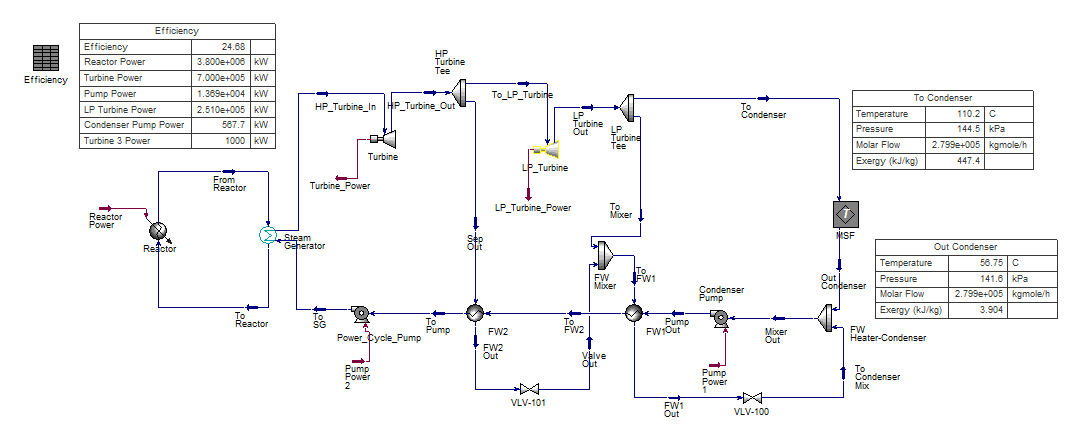
\includegraphics[width=\textwidth]{110PC.PNG}
\caption{\small \sl A much simplified model of the Palo Verde Generating Station's Power Cycle sending 110\degree C heat to the condenser to be used for the multi-stage flash distillation water purification process}
\end{figure*}
\begin{figure*}
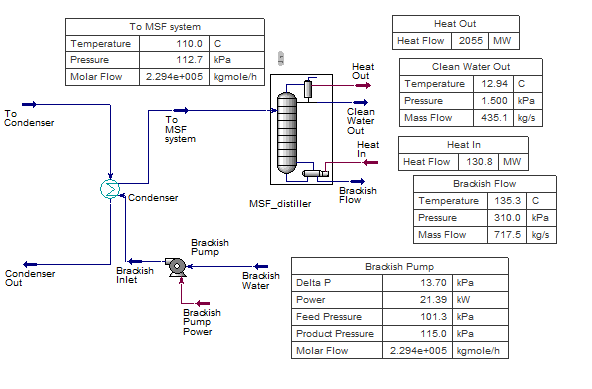
\includegraphics[width=\textwidth]{110MSF.PNG}
\caption{\small \sl A simplified model of a 21 stage multi stage flash distillation system functioning with 110\degree C heat from the reactor to the condenser to be used for the multi-stage flash distillation water purification process}
\end{figure*}

\begin{figure*}
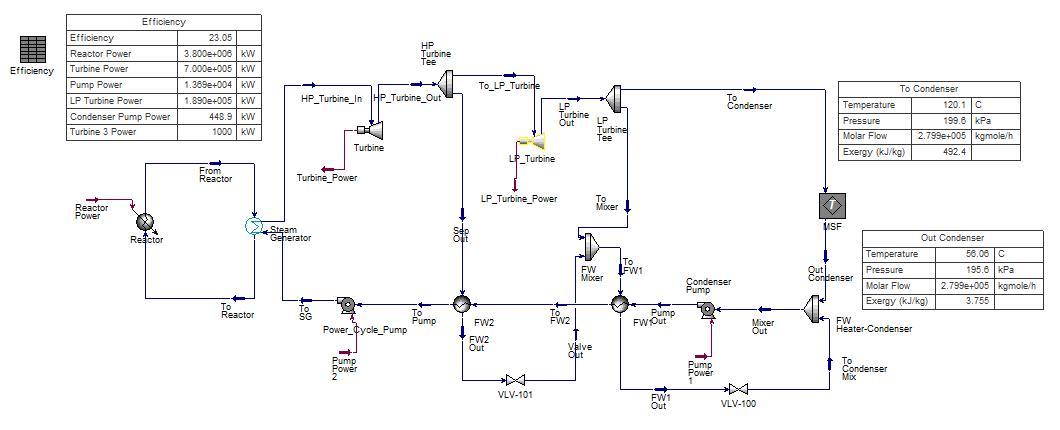
\includegraphics[width=\textwidth]{120PC.PNG}
\caption{\small \sl A much simplified model of the Palo Verde Generating Station's Power Cycle sending 120\degree C heat to the condenser to be used for the multi-stage flash distillation water purification process}
\end{figure*}
\begin{figure*}
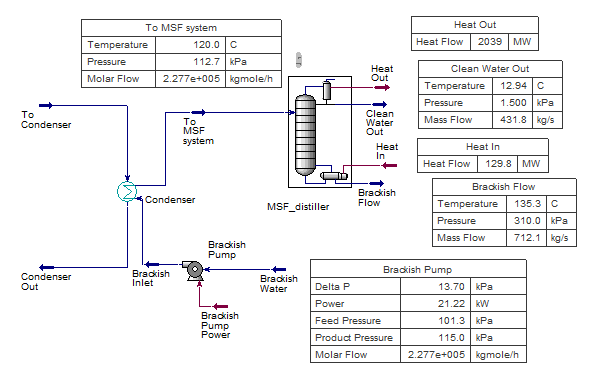
\includegraphics[width=\textwidth]{120MSF.PNG}
\caption{\small \sl A simplified model of a 21 stage multi stage flash distillation system functioning with 120\degree C heat from the reactor to the condenser to be used for the multi-stage flash distillation water purification process}
\end{figure*}
\begin{figure*}
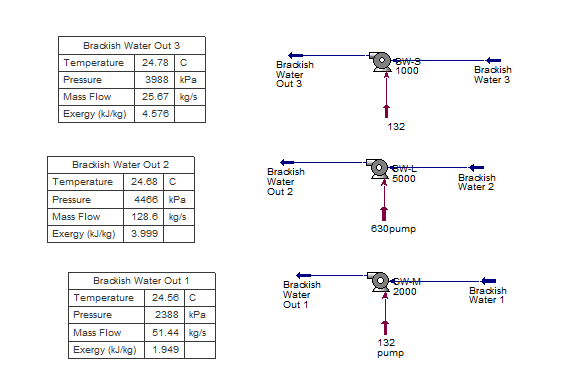
\includegraphics[width=\textwidth]{RO_3Pumps.PNG}
\caption{\small \sl Three pumps which are marketed for reverse osmosis systems by IDE Progreen}
\end{figure*}

\newpage

\chapter{Aspen HYSYS Water Composition Calculation}
In order to assess the purity of the water produced through the MSF system, the water input into the system needed to closely match the brackish groundwater found in Arizona.  In order to demonstrate a worst case scenario, the thesis multiplied the particulates in the system by about 10.  The table below demonstrates the dimensional analysis implemented in order to find the mole percent of each particulate.

\begin{figure}
\centering
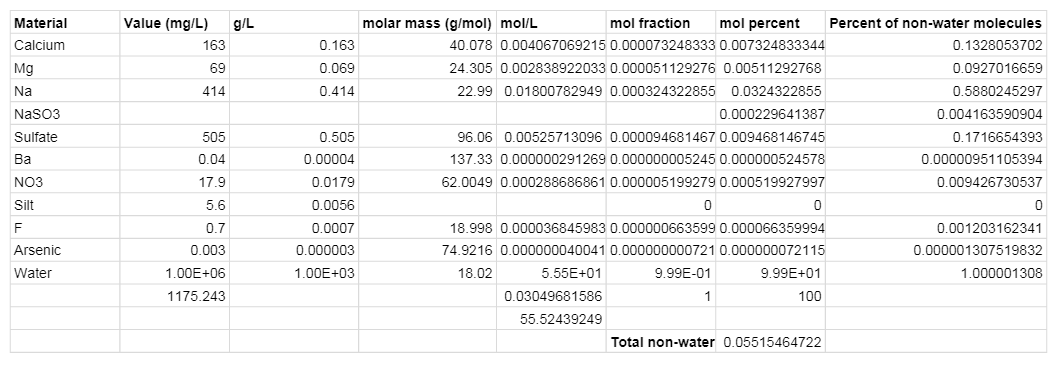
\includegraphics[width=.9\textwidth]{watercalc.PNG}
\caption{\small \sl Screen shot of Excel Calculation of the component makeup for the brackish underground water in Arizona}
\end{figure}

% \chapter{Economic Calculations}
% The economic calculations

% \includepdf[pages={1-}]{CleanedUpData.pdf}

\chapter{RAVEN Input Code}
The following code displays how the Arizona Public Service's hourly demand data was initially translated into daily time series in the eia datetime general python code.  Then, the convert multiple histories code displays taking the data and separating it into the seasons as defined by the Farmer's Almanac.  Finally, the train eia xml document displays the RAVEN input document for one season, in this case fall.  This xml document shows how the data is input into the system, which then trains the ARMA model to have similar statistical outcomes as the real data input into the system.  Finally, the Arizona fall document generates the synthetic data and plots it in the graphs included in this thesis.

\includepdf{eia_data_python.pdf}
\includepdf{convert_multiple_histories.pdf}
\includepdf{RAVEN_APS_train_eia_fall.pdf}
\includepdf{RAVEN_APS_Arizona_fall.pdf}




% Below are the examples of code listings that Christopher Goes, Matthew Brown, Cara Leatherman, and
  % Chris Zeoli put together. First is a YAML file listing, which has a definition in the .cls file.
  % Listings can be anything, e.g full experiment results, a list of equipment used, etc. It is just
  % really handy for formatting code. To see how to define new code languages, see the .cls file.

% \chapter{Invoice}
% \label{appx:Invoice}
% \lstinputlisting[firstline=1, firstnumber=1, language=yaml, caption=Invoice]{Code/example.yaml}

% Example of a Python script code listing, but without the example file or specification. Included
  % to see the differences between the two languages
% \chapter{vsphere-info Script Source Code}
% \lstinputlisting[firstline=16, firstnumber=1, language=python, caption=vsphere-info script]{Code/vsphere_info.py}

% ============================================= END ============================================== %
% Finishes up the document. Necessary line to compile your thesis.
\end{document}

% DO NOT PUT ANYTHING BESIDES COMMENTS AFTER THE END OF THE DOCUMENT! %
% A final tip: if you need to cut something out of your paper, rather than delete it, it's a good idea to move the text to another place. I like to have a scratch.tex file for this. Such a file is also pretty helpful for creating an outline, or quickly laying out ideas.
